\documentclass[a4paper]{article}

\def\nbook {Differential Equations and Linear Algebra}
\def\nbookshort {DeqLA}

%%%%%%%%%%%%%%%%%%%%
% AUTHOR AND HEADER
% define \nbook
%%%%%%%%%%%%%%%%%%%%

\makeatletter
\ifx \nauthor\undefined
	\def\nauthor{David A. Lee}
\else
\fi

\author{\nbook \\ \small Gilbert Strang \\ \small Solutions by \nauthor}
\date{}

%%%%%%%%%%%%%%%%%%%%
% PACKAGES
%%%%%%%%%%%%%%%%%%%%

\usepackage{alltt} 
\usepackage{amsfonts}
\usepackage{amsmath}
\usepackage{amssymb}
\usepackage{amsthm}
\usepackage{bm}
\usepackage{booktabs}
\usepackage{caption}
\usepackage{centernot}
\usepackage{enumitem}
\usepackage{fancyhdr}
\usepackage[T1]{fontenc}
\usepackage{graphicx}
\usepackage{mathdots}
\usepackage{mathtools}
\usepackage{microtype}
\usepackage{multirow}
\usepackage{pdflscape}
\usepackage{pgfplots}
\pgfplotsset{compat=1.18}
\usepackage{siunitx}
\usepackage{slashed}
\usepackage{tabularx}
\usepackage{tikz}
\usepackage{titletoc}
\usepackage{tkz-euclide}
\usepackage[normalem]{ulem}
\usepackage{url}
\usepackage[all]{xy}
\usepackage{imakeidx}

% fonts
% use \textsf to change to Computer Modern Bright
\renewcommand{\sfdefault}{cmbr} % keeps default font Computer Modern Roman

% makeindex for table of contents
\makeindex[intoc, title=Index]
\indexsetup{othercode={\lhead{ Index }}}

% table of contents remove numbering
\usepackage{tocloft} % for coloring subsections -- note that sections have standard document hyperlink coloring, i.e. color = doc
\setcounter{secnumdepth}{0} % remove numbering
\renewcommand{\cftsubsecfont}{\hypersetup{linkcolor=subsect!90}} % subsection coloring
\renewcommand{\contentsname}{\textsf{Table of Contents}}

% pagestyle
\pagestyle{fancyplain}

% header
\lhead{	\nouppercase{\leftmark} }
\ifx \nextra \undefined
  \rhead{
    \ifnum\thepage=1
    \else
      \nbookshort \  | \nauthor
    \fi}
\else
  \rhead{
    \ifnum\thepage=1
    \else
      \nbookshort (\nextra)
    \fi}
\fi

% proof environment

\newcommand{\prooffont}{\scshape}
\usepackage{xpatch}
\tracingpatches
\xpatchcmd{\proof}{\itshape}{\prooffont}{}{}

% Python environment (for typesetting Python code)

% Default fixed font does not support bold face
\DeclareFixedFont{\ttb}{T1}{txtt}{bx}{n}{8} % for bold
\DeclareFixedFont{\ttm}{T1}{txtt}{m}{n}{8}  % for normal

% Custom colors
\usepackage{color}
\definecolor{deepblue}{rgb}{0,0,0.5}
\definecolor{deepred}{rgb}{0.6,0,0}
\definecolor{deepgreen}{rgb}{0,0.5,0}

\usepackage{listings}

% Python style for highlighting
\newcommand\pythonstyle{\lstset{
language=Python,
basicstyle=\ttm,
morekeywords={self},              % Add keywords here
keywordstyle=\ttb\color{deepblue},
emph={MyClass,__init__},          % Custom highlighting
emphstyle=\ttb\color{deepred},    % Custom highlighting style
stringstyle=\color{deepgreen},
frame=tb,                         % Any extra options here
showstringspaces=false
}}


% Python environment
\lstnewenvironment{python}[1][]
{
\pythonstyle
\lstset{#1}
}
{}

% Python for external files
\newcommand\pythonexternal[2][]{{
\pythonstyle
\lstinputlisting[#1]{#2}}}

% Python for inline
\newcommand\pythoninline[1]{{\pythonstyle\lstinline!#1!}}

%%%%%%%%%%%%%
% FUNCTIONS %
%%%%%%%%%%%%%

\DeclarePairedDelimiter\abs{\lvert}{\rvert}%
\DeclarePairedDelimiter\norm{\lVert}{\rVert}%

%%%%%%%%%%%%%%%%%%%%
% DOCUMENT GEOMETRY
%%%%%%%%%%%%%%%%%%%%

\ifx \ntrim \undefined
\else
  \usepackage{geometry}
  \geometry{
	  papersize={379pt, 699pt},
	  textwidth=345pt,
	  left=17pt,
	  top=54pt,
	  right=17pt,
  }
\fi

% maketitle statement
\title{}
\ifx \nisofficial \undefined
\let\@real@maketitle\maketitle
\renewcommand{\maketitle}{\@real@maketitle\begin{center}\begin{minipage}[c]{0.9\textwidth}\centering\footnotesize All errors, typographical and substantive, and other offenses, are entirely my own.\end{minipage}\end{center}}
\else
\fi

%%%%%%%%%%%%%%%%%%%%
% THEOREMS
%%%%%%%%%%%%%%%%%%%%

%\theoremstyle{definition}
\newtheorem*{axiom}{Axiom}
\newtheorem*{claim}{Claim}
\newtheorem*{conjecture}{Conjecture}
\newtheorem*{cor}{Corollary}
%\newtheorem*{dfn}{Definition}
\newtheorem*{eg}{Example}
\newtheorem*{ex}{Exercise}
%\newtheorem*{lemma}{Lemma}
\newtheorem*{prop}{Proposition}
%\newtheorem*{thm}{Theorem}
\newtheorem*{remark}{Remark}
\newtheorem*{warning}{Warning}

%%%%%%%%%%%%%%%%%%%%
% FORMATTING AESTHETICS
%%%%%%%%%%%%%%%%%%%%

% itemize bullets
\renewcommand{\labelitemi}{-}
\renewcommand{\labelitemii}{$\circ$}
\renewcommand{\labelenumi}{(\roman{*})}

% new page section
%\let\stdsection\section
%\renewcommand\section{\newpage\stdsection}

% new page subsection
%\let\stdsubsection\subsection
%\renewcommand\subsection{\newpage\stdsubsection}

%%%%%%%%%%%%%%%%%%%%
% \mathbb commands
%%%%%%%%%%%%%%%%%%%%

\newcommand{\C}{\mathbb{C}}
\newcommand{\N}{\mathbb{N}}
\newcommand{\Q}{\mathbb{Q}}
\newcommand{\R}{\mathbb{R}}
\newcommand{\Z}{\mathbb{Z}}

%%%%%%%%%%%%%%%%%%%%
% Complex Numbers
%%%%%%%%%%%%%%%%%%%%

\DeclareMathOperator{\Real}{Re}
\DeclareMathOperator{\Imag}{Im}

%%%%%%%%%%%%%%%%%%%%
% Probability Operators
%%%%%%%%%%%%%%%%%%%%

\DeclareMathOperator{\Bernoulli}{Bernoulli}
\DeclareMathOperator{\betaD}{Beta}
\DeclareMathOperator{\bias}{\textsf{bias}}
\DeclareMathOperator{\binomial}{Binomial}
\DeclareMathOperator{\corr}{Corr}
\DeclareMathOperator{\cov}{\textsf{Cov}}
\DeclareMathOperator{\Exp}{Exp}
\DeclareMathOperator{\gammaD}{Gamma}
\DeclareMathOperator{\mse}{\textsf{MSE}}
\DeclareMathOperator{\multinomial}{Multinomial}
\DeclareMathOperator{\Poisson}{Poisson}
\DeclareMathOperator{\sd}{sd}
\DeclareMathOperator{\se}{\textsf{se}}
\DeclareMathOperator{\Uniform}{Uniform}
\newcommand{\Prob}{\mathbb{P}}
\newcommand{\var}{\mathbb{V}}
\newcommand{\E}{\mathbb{E}}

%%%%%%%%%%%%%%%%%%%%
% TCOLORBOX CODE FROM SeniorMars
%%%%%%%%%%%%%%%%%%%%

%\usepackage[varbb]{newpxmath} changes math font to newpxmath
\usepackage{xfrac}
\usepackage[makeroom]{cancel}
\usepackage{mathtools}
\usepackage{bookmark}
\usepackage{enumitem}
\usepackage{hyperref}
\usepackage{theoremref}
\hypersetup{
	pdftitle={Assignment},
	colorlinks=true, linkcolor=doc!90,
	bookmarksnumbered=true,
	bookmarksopen=true
}
\usepackage[most,many,breakable]{tcolorbox}
\usepackage{xcolor}
\usepackage{varwidth}
\usepackage{varwidth}
\usepackage{etoolbox}
%\usepackage{authblk}
\usepackage{nameref}
\usepackage{multicol,array}
\usepackage{tikz-cd}
\usepackage[ruled,vlined,linesnumbered]{algorithm2e}
\usepackage{comment} % enables the use of multi-line comments (\ifx \fi)
\usepackage{import}
\usepackage{xifthen}
\usepackage{pdfpages}
\usepackage{transparent}

\newcommand\mycommfont[1]{\footnotesize\ttfamily\textcolor{blue}{#1}}
\SetCommentSty{mycommfont}
\newcommand{\incfig}[1]{%
    \def\svgwidth{\columnwidth}
    \import{./figures/}{#1.pdf_tex}
}

\usepackage{tikzsymbols}

% colors -- change them as you may!

\definecolor{myg}{RGB}{56, 140, 70}
\definecolor{myb}{RGB}{45, 111, 177}
\definecolor{myr}{RGB}{199, 68, 64}
\definecolor{mytheorembg}{HTML}{F2F2F9}
\definecolor{mytheoremfr}{HTML}{00007B}
\definecolor{mylenmabg}{HTML}{FFFAF8}
\definecolor{mylenmafr}{HTML}{983b0f}
\definecolor{mypropbg}{HTML}{f2fbfc}
\definecolor{mypropfr}{HTML}{191971}
\definecolor{myexamplebg}{HTML}{F2FBF8}
\definecolor{myexamplefr}{HTML}{88D6D1}
\definecolor{myexampleti}{HTML}{2A7F7F}
\definecolor{mydefinitbg}{HTML}{E5E5FF}
\definecolor{mydefinitfr}{HTML}{3F3FA3}
\definecolor{notesgreen}{RGB}{0,162,0}
\definecolor{myp}{RGB}{197, 92, 212}
\definecolor{mygr}{HTML}{880808}
\definecolor{myred}{RGB}{127,0,0}
\definecolor{myyellow}{RGB}{169,121,69}
\definecolor{myexercisebg}{HTML}{F2FBF8}
\definecolor{myexercisefg}{HTML}{88D6D1}
\definecolor{doc}{RGB}{0,0,255}
\definecolor{subsect}{RGB}{255,0,0}
\definecolor{question}{HTML}{3FB69E}

%================================
% THEOREM BOX
%================================

%\providecommand\theoremnumber{}
\tcbuselibrary{theorems,skins,hooks}
\newtcbtheorem{Theorem}{Theorem}
{%
	enhanced,
	breakable,
	colback = mytheorembg,
	frame hidden,
	boxrule = 0sp,
	borderline west = {2pt}{0pt}{mytheoremfr},
	sharp corners,
	detach title,
	before upper = \tcbtitle\par\smallskip,
	coltitle = mytheoremfr,
	fonttitle = \bfseries\sffamily,
	description font = \mdseries,
	separator sign none,
	segmentation style={solid, mytheoremfr},
}
{th}


%================================
% Question BOX
%================================

\makeatletter
\newtcbtheorem{question}{Question}{enhanced,
	breakable,
	colback=white,
	colframe=question,
	attach boxed title to top left={yshift*=-\tcboxedtitleheight},
	fonttitle=\bfseries\sffamily,
	title={#2},
	boxed title size=title,
	boxed title style={%
			sharp corners,
			rounded corners=northwest,
			colback=tcbcolframe,
			boxrule=0pt,
		},
	underlay boxed title={%
			\path[fill=tcbcolframe] (title.south west)--(title.south east)
			to[out=0, in=180] ([xshift=5mm]title.east)--
			(title.center-|frame.east)
			[rounded corners=\kvtcb@arc] |-
			(frame.north) -| cycle;
		},
	#1
}{def}
\makeatother

%================================
% PROPERTIES BOX
%================================

\tcbuselibrary{theorems,skins,hooks}
\newtcbtheorem{Property}{Property}
{%
	enhanced,
	breakable,
	colback = mytheorembg,
	frame hidden,
	boxrule = 0sp,
	borderline west = {2pt}{0pt}{mytheoremfr},
	sharp corners,
	detach title,
	before upper = \tcbtitle\par\smallskip,
	coltitle = mytheoremfr,
	fonttitle = \bfseries\sffamily,
	description font = \mdseries,
	separator sign none,
	segmentation style={solid, mytheoremfr},
}
{th}

%================================
% LEMMA
%================================

\tcbuselibrary{theorems,skins,hooks}
\newtcbtheorem[number within=section]{Lemma}{Lemma}
{%
	enhanced,
	breakable,
	colback = mylenmabg,
	frame hidden,
	boxrule = 0sp,
	borderline west = {2pt}{0pt}{mylenmafr},
	sharp corners,
	detach title,
	before upper = \tcbtitle\par\smallskip,
	coltitle = mylenmafr,
	fonttitle = \bfseries\sffamily,
	description font = \mdseries,
	separator sign none,
	segmentation style={solid, mylenmafr},
}
{th}


% Commands for special boxes
\newcommand{\thm}[2]{\begin{Theorem*}{#1}{}#2\end{Theorem*}}
\newcommand{\qs}[2]{\begin{question*}{#1}{}#2\end{question*}}
\newcommand{\prp}[2]{\begin{Property*}{#1}{}#2\end{Property*}}
\newcommand{\lemma}[2]{\begin{Lemma*}{#1}{}#2\end{Lemma*}}


\begin{document}
\maketitle

\newpage
\tableofcontents

\newpage
\section{\textsf{1 - First Order Equations}}

\subsection{\textsf{1.1 - Four Examples: Linear versus Nonlinear}}
% QUESTION 1
\qs{1.1.1}{Draw the graph of \(y = e^{t}\) by hand, for \(-1 \le t \le 1\). What is its slope \(dy / dt\) at \(t = 0\)? Add the straight line graph of \(y = et\). Where do those two graphs cross?}

At \(t=0\), \(dy / dt = e^{0} = 1\). The functions \(y = e^{t}\) and \(y = et\) meet at \(\!\left( 1, e \right) \).

\begin{center}
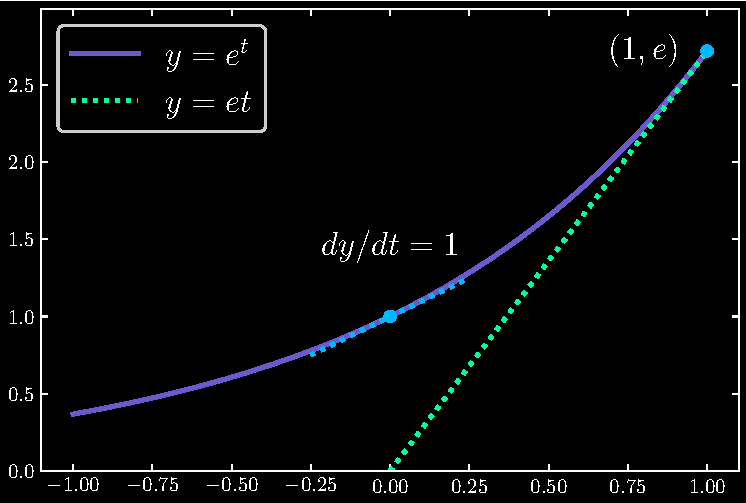
\includegraphics[width=1.0\textwidth]{chap1/sec1.1/chap1sec1.1ex1.eps}
\end{center}

% QUESTION 2
\qs{1.1.2}{Draw the graph of \(y_{1} = e^{2t}\) on top of \(y_{2} = 2 e^{t}\). Which function is larger at \(t=0\)? Which function is larger at \(t=1\)?}

At \(t=0\), \(y_{2} > y_{1}\). At \(t=1\), \(y_{1} > y_{2}\).

\begin{center}
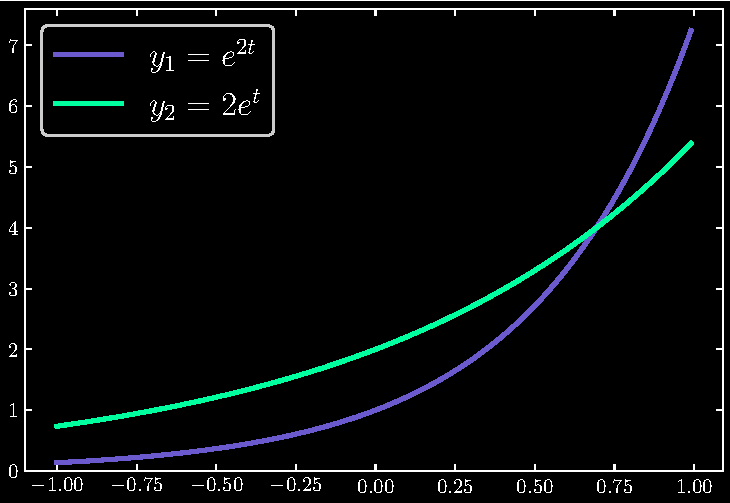
\includegraphics[width=1.0\textwidth]{chap1/sec1.1/chap1sec1.1ex2.eps}
\end{center}

% QUESTION 3
\qs{1.1.3}{What is the slope of \(y=e^{-t}\) at \(t=0\)? Find the slope \(dy/dt\) at \(t=1\).}

Calculate \(dy/dt = -e^{-t}\). Then 
\begin{align*}
	\frac{d y}{d t}_{\!\left( t=0 \right) } &= -e^{0} = -1 \\
	\frac{d y}{d t}_{\!\left( t=1 \right) } &= -e^{-1}
\end{align*}

% QUESTION 4
\qs{1.1.4}{What "logarithm" do we use for the number \(t\) (the exponent) when \(e^{t} = 4\)?}

The natural logarithm: \(\ln\!\left( e^{t} \right) = \ln\!\left( 4 \right)\) implies \(t = \ln\!\left( 4 \right)\).

\vspace{12pt}

% QUESTION 5
\qs{1.1.5}{State the chain rule for the derivative \(dy/dt\) if \(y \!\left( t \right) = f \!\left( u \!\left( t \right)  \right) \) (chain of \(f\) and \(u\)).}
\[
	\frac{d }{d t} y \!\left( t \right) = \frac{d f}{d u}_{\!\left( u \!\left( t \right)  \right)} \cdot \frac{d u}{d t}  
\]

% QUESTION 6
\qs{1.1.6}{The \textit{second} derivative of \(e^{t}\) is again \(e^{t}\). So \(y=e^{t}\) solves \(d^{2}y/dt^{2} = y\). A second order differential equation should have another solution, different from \(y=Ce^{t}\). What is that second solution?}

Since \(y = e^{-t}\) has second derivative \(d^{2}y/dt^{2} = e^{-t}\), we must have as our second solution \(y = De^{-t}\).

\vspace{12pt}

% QUESTION 7
\qs{1.1.7}{Show that the nonlinear example \(dy/dt = y^{2}\) is solved by \(y = C / \!\left( 1 - Ct \right) \) for every constant \(C\). The choice \(C = 1\) gave \(y = 1 / \!\left( 1-t \right) \), starting from \(y \!\left( 0 \right) = 1\).}
For \(y = C / \!\left( 1 - Ct \right) \), we have
\[
	\frac{d y}{d t} = - \!\left( \frac{1}{1-Ct} \right)^{2}  C	 \!\left( -C \right) = \!\left( \frac{C}{1-Ct} \right)^{2} = y^{2}
\]	

% QUESTION 8
\qs{1.1.8}{Why will the solution to \(dy/dt = y^{2}\) grow faster than the solution to \(dy/dt = y\) (if we start them both from \(y=1\) at \(t=0\))? The first solution blows up at \(t=1\). The second solution \(e^{t}\) grows exponentially fast but it never blows up.}

Observe that
\[
	\lim\limits_{t^{-} \to 1} \frac{1}{1-t} = +\infty
\]
Hence the first solution grows considerably faster than the second solution as \(t\) approaches \(1\).

\begin{center}
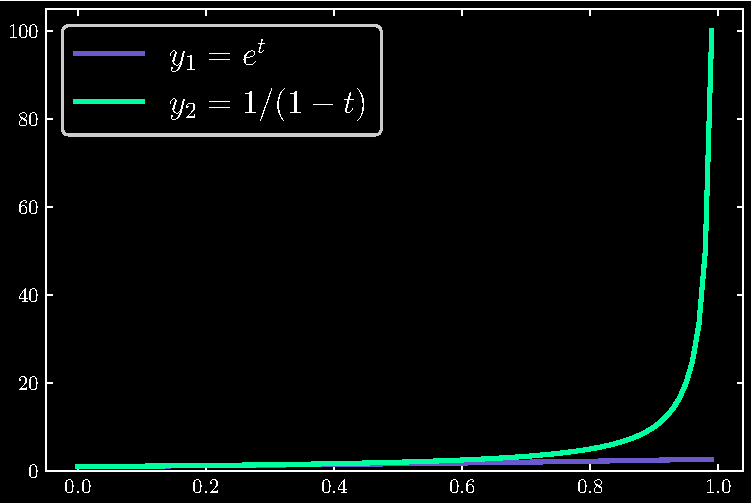
\includegraphics[width=1.0\textwidth]{chap1/sec1.1/chap1sec1.1ex8.eps}
\end{center}

\qs{1.1.9}{Find a solution to \(dy/dt = -y^{2}\) starting from \(y \!\left( 0 \right) = 1\). Integrate \(dy/y^{2}\) and \(-dt\). (Or work with \(z = 1/y\). Then \(\bm{dz/dt} = \!\left( dz/dy \right) \!\left( dy/dt \right) = \!\left( -1/y^{2} \right) \!\left( -y^{2} \right) = \textbf{1}\). From \(dz/dt = 1\) you will know \(z \!\left( t \right) \) and \(y = 1/z\).}

\underline{Solution 1.} Write
\begin{alignat*}{2}
	&-\int \frac{1}{y^{2}} \ dy  && = \int  \ dt  \\
	&\implies y^{-1} && = t + C \\ 
	&\implies y && = \boxed{\frac{1}{t + C}, \quad C = 1}
\end{alignat*}

\underline{Solution 2.} Let \(z = 1/y\). Then
\[
	\frac{d z}{d t} = \frac{d z}{d y} \frac{d y}{d t} = \!\left( -\frac{1}{y^{2}} \right) \!\left( -y^{2} \right) = 1
\]
Since \(dz/dt = 1\),
\begin{align*}
	\int \ dz = \int \ dt & \implies z = t + C \\
	 & \implies \frac{1}{y} = t + C \\ 
	 & \implies \boxed{y = \frac{1}{t + C}, \quad C = 1}
\end{align*}

% QUESTION 10
\qs{1.1.10}{Which of these differential equations are linear (in \(y\))?\begin{enumerate}[label=(\alph*)]
	\item \(y' + \sin y = t\)
	\item \(y' = t^{2} \!\left( y-t \right) \)
	\item \(y' + e^{t}y = t^{10}\)
\end{enumerate}}

Only (b) and (c) are linear in \(y\).

\vspace{12pt}

% QUESTION 11
\qs{1.1.11}{The product rule gives what derivative for \(e^{t} e^{-t}\)? This function is constant. At \(t=0\) this constant is \(1\). Then \(e^{t}e^{-t} = 1\) for all \(t\).}

By the product rule, we have
\begin{align*}
	\frac{d }{d t} \!\left( e^{t}e^{-t} \right)  & = e^{-t} \frac{d }{d t} \!\left( e^{t} \right) + e^{t} \frac{d }{d t} \!\left( e^{-t} \right)  \\
	 & = \!\left( e^{-t} \right) \!\left( e^{t} \right) - \!\left( e^{t} \right) \!\left( e^{-t} \right)  \\ 
	 & = 0
\end{align*}

which aligns with the result that \(d(1)/dt = 0\).

% QUESTION 12
\qs{1.1.12}{\(dy/dt = y + 1\) is not solved by \(y = e^{t} + t\). Substitute that \(y\) to show it fails. We can't just add the solutions to \(y' = y\) and \(y' = 1\). What number \(c\) makes \(y = e^{t} + c\) into a correct solution?}

Observe that
\begin{align*}
	\frac{d }{d t} \!\left( e^{t} + t \right)   & = e^{t} + 1 \\
	 & \neq e^{t} + t + 1 \\ 
\end{align*}

If \(c = -1\), we have
\begin{align*}
	\frac{d }{d t} \!\left( e^{t} - 1 \right)   & = e^{t} \\
	 & = \!\left( e^{t} - 1 \right) + 1  \\ 
\end{align*}

\newpage
\subsection{\textsf{1.3 - The Exponentials \texorpdfstring{\(e^{t}\)}{e(t)} and \texorpdfstring{\(e^{at}\)}{exp(at)}}}

% QUESTION 1
\qs{1.3.1}{Set \(t = 2\) in the infinite series for \(e^{2}\). The sum must be \(e\) times \(e\), close to \(7.39\). How many terms in the series to reach a sum of \(7\)? How many terms to pass \(7.3\)?}

Five terms are needed to reach 7 exactly:
\[
	y = 1 + t + \frac{1}{2!}t^{2} + \frac{1}{3!}t^{3} + \frac{1}{4!}t^{4} = 7
\]
And seven terms to surpass 7.3:
\[
	y = 1 + t + \frac{1}{2!}t^{2} + \frac{1}{3!}t^{3} + \frac{1}{4!}t^{4} + \frac{1}{5!}t^{5} + \frac{1}{6!}t^{6} \approx 7.36
\]

\begin{python}
t = 2

term1 = 1
term2 = 1 + t
term3 = 1 + t + (1/2)*np.power(t,2)
term4 = 1 + t + (1/2)*np.power(t,2) + (1/6)*np.power(t,3)
term5 = 1 + t + (1/2)*np.power(t,2) + (1/6)*np.power(t,3) 
	+ (1/24)*np.power(t,4)
term6 = 1 + t + (1/2)*np.power(t,2) + (1/6)*np.power(t,3) 
	+ (1/24)*np.power(t,4) + (1/120)*np.power(t,5)
term7 = 1 + t + (1/2)*np.power(t,2) + (1/6)*np.power(t,3) 
	+ (1/24)*np.power(t,4) + (1/120)*np.power(t,5) 
	+ (1/720)*np.power(t,6)
\end{python}

% QUESTION 2
\qs{1.3.2}{Starting from \(y \!\left( 0 \right) = 1\), find the solution to \(dy/dt = y\) at time \(t = 1\). Starting from that \(y \!\left( 1 \right) \), solve \(dy/dt = -y\) to time \(t = 2\). Draw a rough graph of \(y \!\left( t \right) \) from \(t = 0\) to \(t = 2\). What does this say about \(e^{-1}\) times \(e\)?}

The solution to \(dy/dt = y\) is \(y = Ce^{t}\); since by premise we have \(y \!\left( 0 \right) = 1\), this implies \(C = 1\). Moreover, we have \(y \!\left( 1 \right) = e\). For \(dy/dt = -y\), we have solution \(y = De^{-t}\). Using \(y \!\left( 1 \right) = e\), we may conclude \(D = e^{2}\). Thus at \(t = 2\), \(y \!\left( 2 \right) = 1\). The complete solution is
\[
	y \!\left( t \right) =
	\begin{cases}
		e^{t} & 0 \le t \le 1 \\
		e^{2-t} & 1 < t \le 2 \\
	\end{cases}
\]
Graphically, we have:

\begin{center}
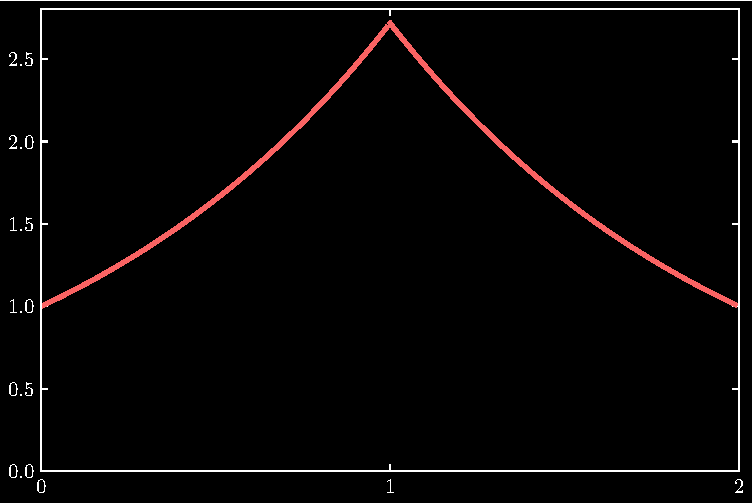
\includegraphics[width=1.0\textwidth]{chap1/sec1.3/chap1sec1.3ex2.eps}
\end{center}

This implies that \(e^{-1} \cdot e = 1\).

\vspace{12pt}

% QUESTION 3
\qs{1.3.3}{Start with \(y \!\left( 0 \right) = \$5000\). If this grows by \(dy/dt = .02y\) until \(t = 5\) and then jumps to \(a = .04\) per year until \(t = 10\), what is the account balance at \(t = 10\)?}

The solution to \(dy/dt = .02y\) with \(y_{1} \!\left( 0 \right) = 5000\) is \(y_{1} = 5000e^{.02t}\), for \(0 \le t \le 5\). 

When the interest rate changes to \(.04\) at \(t = 5\), we must solve \(dy/dt = .04y\) and impose the initial constraint that \(y_{2} \!\left( 5 \right) = y_{1} \!\left( 5 \right) \). We can conclude that \(y_{2}\) is
\[
	y_{2} \!\left( t \right) = \!\left( \frac{5000e^{.02 \cdot 5}}{e^{.04 \cdot 5}} \right) e^{.04t} = \!\left( 5000e^{-.1} \right) e^{.04t} , \quad 5 < t \le 10
\]
Lastly, we calculate that at \(t = 10\), \(y \!\left( 10 \right) = \$6749.29\). Graphically, we have

\begin{center}
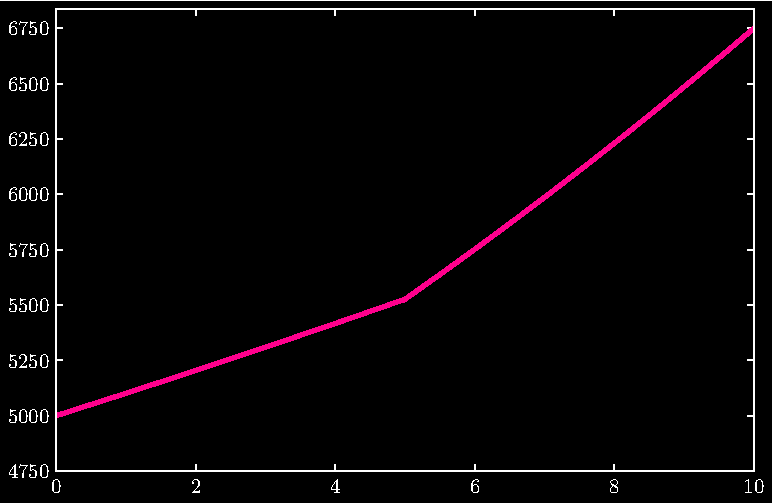
\includegraphics[width=1.0\textwidth]{chap1/sec1.3/chap1sec1.3ex3.eps}
\end{center}

% QUESTION 4
\qs{1.3.4}{Change Problem 3 to start with \(\$5000\) growing at \(dy/dt = .04y\) for the first five years. Then drop to \(a = .02\) until \(t = 10\). What is now the balance at \(t = 10\)?}

Switching \(.02\) and \(.04\) in the previous problem, we derive the exact same balance of \(y \!\left( 10 \right) = \$6749.29\). The piecewise solutions are
\[
	y \!\left( t \right) =
	\begin{cases}
		y_{1} \!\left( t \right)  = 5000e^{.04t} & 0 \le t \le 5 \\
		y_{2} \!\left( t \right)  = \!\left( \frac{5000e^{.04 \cdot 5}}{e^{.02 \cdot 5}} \right) e^{.02t} & 5 < t \le 10 \\
	\end{cases}
\]

Graphically, we have

\begin{center}
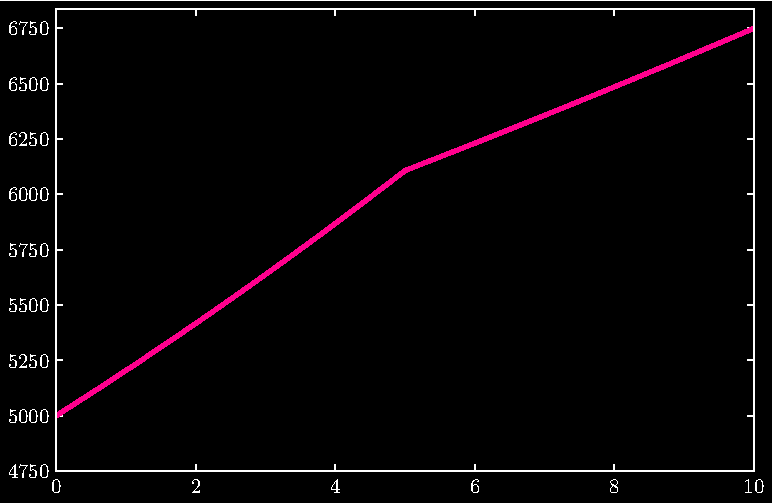
\includegraphics[width=1.0\textwidth]{chap1/sec1.3/chap1sec1.3ex4.eps}
\end{center}

% QUESTION 5
\qs{1.3.5}{Replace \(t\) by \(at\) in the exponential series to find \(e^{at}\):
\[
	e^{at} = 1 + at + \frac{1}{2} \!\left( at \right)^{2} + \cdots + \frac{1}{n!} \!\left( at \right)^{n} + \cdots 
\]
Take the derivative of every term (keep five terms). Factor out \(a\) to show that \textit{the derivative of \(e^{at}\) equals \(ae^{at}\)}. At what time \(T\) does \(e^{at}\) reach 2?}

Derive
\begin{align*}
	\frac{d }{d t} e^{at} &= a + a \!\left( at \right) + \cdots + \frac{1}{\!\left( n-1 \right)!} a \!\left( at \right)^{n-1} + \cdots \\
			     &= a \!\left( 1 + at + \cdots + \frac{1}{\!\left( n-1 \right)!} \!\left( at \right)^{n-1} + \cdots \right) \\
			     &= ae^{at}
\end{align*}

For \(e^{aT} = 2\), calculate
\begin{alignat*}{2}
	\implies& aT && = \ln\!\left( 2 \right) \\
	\implies& T && = \boxed{ \frac{\ln\!\left( 2 \right)}{a} } \\ 
\end{alignat*}

\newpage
% QUESTION 6
\qs{1.3.6}{Start from \(y' = ay\). Take the derivative of that equation. Take the \(n^{\text{th}}\) derivative. Construct the Taylor series that matches all these derivatives at \(t = 0\), starting from \(1 + at + \frac{1}{2} \!\left( at \right)^{2}\). Confirm that this series for \(y \!\left( t \right) \) is the series for \(e^{at}\) in Problem 5.}

The derivative of \(y' = ay\) is:
\[
	y'' = ay'
\]
The \(n^{\textit{th}}\) derivative is:
\[
	y^{\!\left( n + 1 \right) } = ay^{\!\left( n \right) }
\]
Starting from \(1 + at + \frac{1}{2} \!\left( at \right)^{2}\), we observe that
\[
	y' = a + a \!\left( at \right) \quad \text{and} \quad ay = a \!\left( 1 + at + \frac{1}{2} \!\left( at \right)^{2} \right) 
\]
but as it stands, the two sides are unequal. If we add a term \(\frac{1}{3!} \!\left( at \right)^{3}\), we have
\[
	y' = a + a \!\left( at \right) + \frac{1}{2} a \!\left( at \right)^{2} \quad \text{and} \quad ay = a \!\left( 1 + at + \frac{1}{2} \!\left( at \right)^{2} + \frac{1}{3!} \!\left( at \right)^{3} \right) 
\]
In fact, we will need to continue adding terms of the form \(\frac{1}{n!} \!\left( at \right)^{n}\) ad infinitem. Observe that we derive the result of Problem 5 in this manner.

In general, the \(k^{\text{th}}\) derivative of the term \(\frac{1}{n!} \!\left( at \right)^{n}\) is
\[
	\frac{1}{\!\left( n-k \right)!} a^{k} \!\left( at \right)^{n-k}
\]
Then the equation \(y^{\!\left( n + 1 \right)} = ay^{\!\left( n \right) }\) is
\[
	a^{n + 1} + a^{n + 1} \!\left( at \right) + \frac{1}{2!} a^{n + 1} \!\left( at \right)^{2} + \cdots = a \!\left( a^{n} + a^{n} \!\left( at \right) + \frac{1}{2!} a^{n} \!\left( at \right)^{2} + \cdots \right) 
\]

% QUESTION 7
\qs{1.3.7}{At what times \(t\) do these events happen?
\begin{enumerate}[label=(\alph*)]
	\item \(e^{at} = e\)
	\item \(e^{at} = e^{2}\)
	\item \(e^{a \!\left( t + 2 \right) } = e^{at} e^{2a}\).
\end{enumerate}}

\par (a) \(t = 1/a\)
\vspace{12pt}
\par (b) \(t = 2/a\)
\vspace{12pt}
\par (c) \(t \ge 0\)

% QUESTION 8
\qs{1.3.8}{If you multiply the series for \(e^{at}\) in Problem 5 by itself you should get the series for \(e^{2at}\). Multiply the first 3 terms by the same 3 terms to see the first 3 terms in \(e^{2at}\).}
\begin{align*}
	\!\left( 1 + at + \frac{1}{2} \!\left( at \right)^{2} \right)^{2} &= \!\left( 1 + at + \frac{1}{2} \!\left( at \right)^{2} \right)  \\
	 & \quad + at \!\left( 1 + at + \frac{1}{2} \!\left( at \right)^{2} \right)  \\ 
	 & \quad + \frac{1}{2} \!\left( at \right)^{2} \!\left( 1 + at + \frac{1}{2} \!\left( at \right)^{2} \right) \\
	 & = 1 + 2at + 2 \!\left( at \right)^{2} + \!\left( at \right)^{3} + \frac{1}{2} \!\left( at \right)^{4}
\end{align*}

% QUESTION 9
\qs{1.3.9}{(recommended) Find \(y \!\left( t \right) \) if \(dy/dt = ay\) and \(\bm{y \!\left( T \right) = 1}\) (instead of \(y \!\left( 0 \right) = 1\)).}

The general solution is \(y \!\left( t \right) = Ce^{at}\). If \(y \!\left( T \right) = 1\), then \(C = e^{-aT}\).

\vspace{12pt}

% QUESTION 10
\qs{1.3.10}{\begin{enumerate}[label=(\alph*)]
	\item If \(dy/dt = \!\left( \ln 2 \right)y \), explain why \(y \!\left( 1 \right) = 2 y \!\left( 0 \right) \).
	\item If \(dy/dt = - \!\left( \ln 2 \right)y \), how is \(y \!\left( 1 \right) \) related to \(y \!\left( 0 \right) \)?
\end{enumerate}}

\par (a) We have \(y \!\left( t \right) = e^{\!\left( \ln 2 \right) t} = 2^{t}\). Then \(y \!\left( 1 \right) = 2\) and \(y \!\left( 0 \right) = 1\). Thus 
\[
	y \!\left( 1 \right) = 2 y \!\left( 0 \right) 
\]
\par (b) We have \(y \!\left( t \right) = 1/2^{t}\). Then \(y \!\left( 1 \right) = 1/2\) and \(y \!\left( 0 \right) = 1\). Thus 
\[
	2 y \!\left( 1 \right) = y \!\left( 0 \right)
\]

% QUESTION 11
\qs{1.3.11}{In a one-year investment of \(y \!\left( 0 \right) = \$100\), suppose the interest rate jumps from \(6\%\) to \(10 \%\) after six months. Does the equivalent rate for a whole year equal \(8 \%\), or more than \(8 \%\), or less than \(8 \%\)?}

The initial condition \(y \!\left( 0 \right) = \$100\) implies \(C = 100\) for the solution \(y_{1} \!\left( t \right) = Ce^{.06t}\). To find the initial condition on \(y_{2} \!\left( t \right) = De^{.1t}\), we must have
\[
	y_{1} \!\left( 6 \right) = 100e^{.06 \cdot 6} = y_{2} \!\left( 6 \right) = De^{.1 \cdot 6}
\]
implying that \(D = 100 e^{-.24}\). The piecewise solutions are
\[
	y \!\left( t \right) = \begin{cases}
		y_{1} \!\left( t \right) = 100e^{.06t}  & 0 \le t \le 6 \\
		y_{2} \!\left( t \right) = \!\left( 100e^{-.24} \right) e^{.1t} & 6 < t \le 12  \\
	\end{cases}
\]

Now, in the event where the interest rate is 8 percent, we can simply determine that the value of our balance at 12 months is
\[
	y \!\left( 12 \right) = 100e^{.8 \cdot 12} = 100e^{.96}
\]
Similarly, in the first case with the two interest rates, we calculate
\[
	y \!\left( 12 \right) = \!\left( 100e^{-.24} \right) e^{.1 \cdot 12} = 100e^{.96}
\]
demonstrating that the end balances are identical in both schemes. Graphically:

\begin{center}
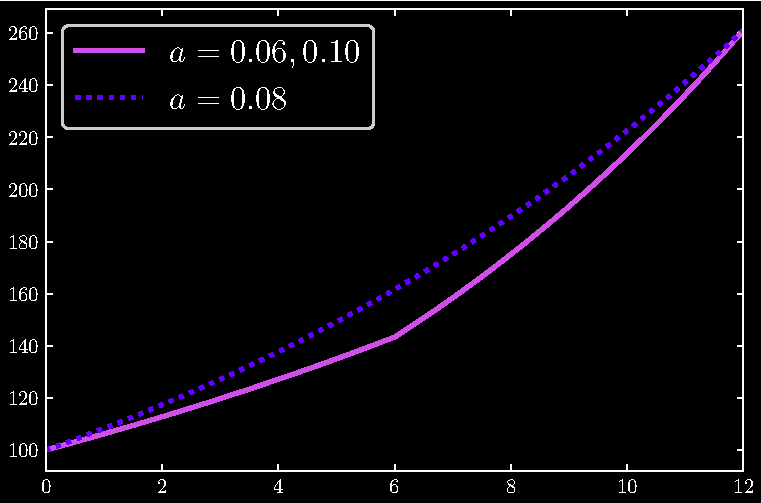
\includegraphics[width=1.0\textwidth]{chap1/sec1.3/chap1sec1.3ex11.eps}
\end{center}

% QUESTION 12
\qs{1.3.12}{If you invest \(y \!\left( 0 \right) = \$100\) at \(4 \%\) interest compounded continuously, then \(dy/dt = .04y\). Why do you have more than \(\$104\) at the end of the year?}

We have solution \(y \!\left( t \right) = 100e^{.04t}\). Since \(e^{.04} > 1.04\), we will have in excess of \(\$104\) at the close of the year.

\vspace{12pt}

\newpage
% QUESTION 13
\qs{1.3.13}{What linear differential equation \(dy/dt = a \!\left( t \right) y\) is satisfied by \(y \!\left( t \right) = e^{\cos t}\)?}

The linear differential equation is satisfied with \(a \!\left( t \right) = -\sin t \).

\vspace{12pt}

% QUESTION 14
\qs{1.3.14}{If the interest rate is \(a = 0.1\) per year in \(y' = ay\), how many years does it take for your investment to be multiplied by \(e\)? How many years to be multiplied by \(e^{2}\)?}

The solution is \(y \!\left( t \right) = C e^{at}\). For any initial investment \(C\), we wish to find \(t_{1}\) such that \(y \!\left( t_{1} \right) = Ce^{at_{1}} = Ce\). It follows that \(t_{1} = 1/a = 10\) years. Similarly, we can derive \(t_{2}\) such that \(y \!\left( t_{2} \right) = Ce^{at_{2}} = Ce^{2}\) as \(t_{2} = 2/a = 20\) years.

\vspace{12pt}

% QUESTION 15
\qs{1.3.15}{Write the first four terms in the series for \(y = e^{t^{2}}\). Check that \(dy/dt = 2ty\).}

By the Taylor series expansion of the exponential function, we have
\begin{align*}
	y = e^{t^{2}} & = 1 + \!\left( t^{2} \right) + \frac{1}{2!} \!\left( t^{2} \right)^{2} + \frac{1}{3!} \!\left( t^{2} \right)^{3} + \cdots \\
		     & = 1 + t^{2} + \frac{1}{2!} t^{4} + \frac{1}{3!} t^{6} + \cdots 
\end{align*}

with derivative
\begin{align*}
	\frac{d y}{d t} & = 2t + \frac{4}{2!} t^{3} + \frac{6}{3!} t^{5} + \frac{8}{4!} t^{7} + \cdots  \\
	 & = 2t \!\left( 1 + t^{2} + \frac{1}{2!} t^{4} + \frac{1}{3!} t^{6} + \cdots  \right)  \\ 
	 & = 2ty
\end{align*}

% QUESTION 16
\qs{1.3.16}{Find the derivative of \(Y \!\left( t \right) = \!\left( 1 + \frac{t}{n} \right)^{n}\). If \(n\) is large, this \(dY/dt\) is close to \(Y\)!}

We have
\[
	\frac{d Y}{d t} = n \!\left( 1 + \frac{t}{n} \right)^{n-1} \!\left( \frac{1}{n} \right) = \!\left( 1 + \frac{t}{n} \right)^{n-1}
\]
As \(n \rightarrow \infty\), \(n \approx n-1\), \(1 + t/n \approx 1\), and \(dY/dt \approx Y\).

% QUESTION 17
\qs{1.3.17}{Suppose the exponent in \(y = e^{u \!\left( t \right) }\) is \(u \!\left( t \right) = \) integral of \(a \!\left( t \right) \). What equation \(dy/dt = \underline{\qquad} \ y\) does this solve? If \(u \!\left( 0 \right) = 0\) what is the starting value \(y \!\left( 0 \right) \)?}

The solution \(y\) solves \(dy/dt = a \!\left( t \right) y\). The initial condition \(u \!\left( 0 \right) = 0\) implies \(y \!\left( 0 \right) = e^{u \!\left( 0 \right) } = 1 \).

\vspace{12pt}

% QUESTION 18
\qs{1.3.18}{\(e^{d/dx} = 1 + d/dx + \frac{1}{2} \!\left( d/dx \right)^{2} + \cdots\) is a sum of higher and higher derivatives. Applying this series to \(f \!\left( x \right) \) at \(x = 0\) would give \(f + f' + \frac{1}{2} f'' + \cdots \) at \(x = 0\). The Taylor series says: This is equal to \(f \!\left( x \right) \) at \(x = \underline{\qquad}\).}

It is clearer if we say that we apply the series to \(f \!\left( a \right) \) at point \(a = 0\). The definition of the Taylor series about the point \(a = 0\) is given by
\[
	\sum_{n=0}^{\infty} \frac{f^{\!\left( n \right) } \!\left( 0 \right) }{n!} x^{n}
\]
Then when \(x = 1\), the Taylor (Maclaurin) series is equal to \(f \!\left( 1 \right) \):
\[
	f \!\left( 1 \right) = f + f' + \frac{1}{2} f'' + \cdots
\]
% QUESTION 19
\qs{1.3.19}{(Computer or calculator, 2.xx is close enough) Find the time \(t\) when \(e^{t} = 10\). The initial \(y \!\left( 0 \right) \) has increased by an order of magnitude - a factor of 10. The exact statement of the answer is \(t = \underline{\qquad}\). At what time \(t\) does \(e^{t}\) reach 100?}

The time \(t\) when \(e^{t} = 10\) is \(t \approx 2.30\). It is exactly \(t = \ln 10\). We reach \(e^{t} = 100\) when \(t = \ln 100 \approx 4.61\).

\vspace{12pt}

% QUESTION 20
\qs{1.3.20}{The most important curve in probability is the bell-shaped graph of \(e^{-t^{2}/2}\). With a calculator or computer find this function at \(t = -2, -1, 0, 1, 2\). Sketch the graph of \(e^{-t^{2}/2}\) from \(t = -\infty\) to \(t = \infty\). \textit{It never goes below zero.}}

The function \(e^{-t^{2}/2}\) at \(t = -2, -1, 0, 1, 2\) is \(0.135, 0.607, 1, 0.607, 0.135\). The graph is

\begin{center}
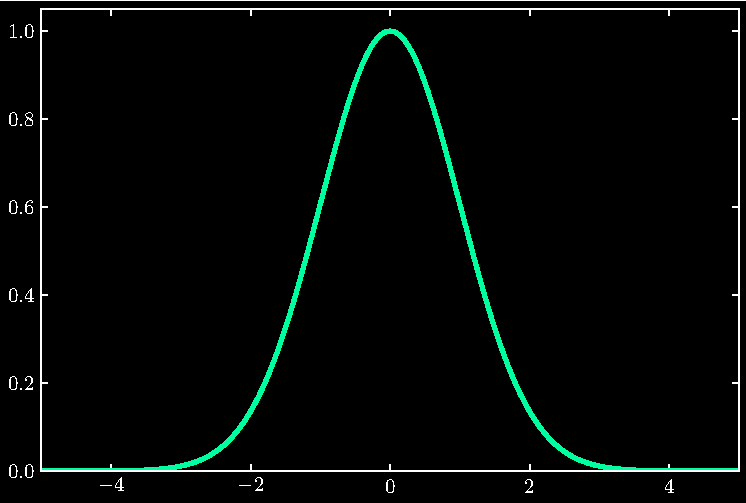
\includegraphics[width=1.0\textwidth]{chap1/sec1.3/chap1sec1.3ex20.eps}
\end{center}

% QUESTION 21
\qs{1.3.21}{Explain why \(y_{1} = e^{\!\left( a + b + c \right) t}\) is the same as \(y_{2} = e^{at} e^{bt} e^{ct}\). They both start at \(y \!\left( 0 \right) = 1.\) They both solve what differential equation?}

Consider the differential equation
\[
	\frac{d y}{d t} = \!\left( a + b + c \right) y
\]
Then by property 1 of the exponential function,
\[
\frac{d y_{1}}{d t} = \!\left( a + b + c\right) e^{\!\left( a + b + c \right)t}  = \!\left( a + b + c \right) y_{1}
\]
Using the product rule, we can also derive from \(y_{2}\):
\begin{align*}
	\frac{d y_{2}}{d t} & = e^{at}e^{bt} \frac{d }{d t} e^{ct} + e^{ct} \frac{d }{d t} \!\left( e^{at}e^{bt} \right) \\
			   & = c y_{2} + e^{ct} \!\left( e^{at} \frac{d }{d t} e^{bt} + e^{bt} \frac{d }{d t} e^{at} \right) \\
			   & = c y_{2} + b y_{2} + a y_{2} \\
			   & = \!\left( a + b + c \right) y_{2}
\end{align*}

ascertaining that \(y_{1} = y_{2}\).

The second method is to begin at \(y \!\left( 0 \right) = 1\), and go to \(e^{at}\). Let \(C = e^{at}\). Then move an additional \(e^{bt}\) and arrive at \(Ce^{bt}\). Let \(D\) equal this, and make one final additional move of \(e^{ct}\). In total, we have grown by a factor of \(e^{at}e^{bt}e^{ct}\). But this is equal to moving ahead in time by \(at + bt + ct = \!\left( a + b + c \right) t\).

% QUESTION 22
\qs{1.3.22}{For \(y' = y\) with \(a = 1\), Euler's first step chooses \(Y_{1} = \!\left( 1 + \Delta t \right) Y_{0} \). Backward Euler chooses \(Y_{1} = Y_{0} / \!\left( 1 - \Delta t \right) \). Explain why \(1 + \Delta t\) is smaller than the exact \(e^{\Delta t}\) and \(1/\!\left( 1 - \Delta t \right) \) is larger than \(e^{\Delta t}\). (Compare the series for \(1/\!\left( 1 - x \right) \) with \(e^{x}\).

\vspace{12pt}
\textbf{Note} Section 3.5 presents an accurate Runge-Kutta method that captures three more terms of \(e^{a \Delta t}\) than Euler. For \(dy/dt = ay\) here is the step to \(Y_{n+1}\):

\vspace{12pt}
\textbf{Runge-Kutta for \(\bm{y' = ay}\)}  
\[
	Y_{n+1} = \!\left( 1 + a \Delta t + \frac{a^{2} \Delta t^{2}}{2} + \frac{a^{3} \Delta t^{3}}{6} + \frac{a^{4} \Delta t^{4}}{24} \right) Y_{n}
\]}

First, observe that
\[
	1 + \Delta t < 1 + \Delta t + \frac{1}{2!} \!\left( \Delta t \right)^{2} + \frac{1}{3!} \!\left( \Delta t \right)^{3} + \cdots = e^{\Delta t}
\]
Allowing us to conclude that \(1 + \Delta t < e^{\Delta t}\).

Next, consider the Taylor series for \(1/\!\left( 1-x \right) \):
\[
	\frac{1}{1-x} = 1 + x + x^{2} + x^{3} + \cdots = \sum_{n=0}^{\infty} x^{n}
\]
Backward Euler gives us
\[
	\frac{1}{1 - \Delta t} = 1 + \Delta t + \!\left( \Delta t \right)^{2} + \!\left( \Delta t \right)^{3} + \cdots 
\]
while the Taylor expansion of \(e^{\Delta t}\) gives us
\[
	e^{\Delta t} = 1 + \Delta t + \frac{1}{2!} \!\left( \Delta t \right)^{2} + \frac{1}{3!} \!\left( \Delta t \right)^{3} + \cdots
\]
which ascertains that \(1 / \!\left( 1 - \Delta t \right) > e^{\Delta t}\). 

\newpage
\subsection{\textsf{1.4 - Four Particular Solutions}}

% QUESTION 1
\qs{1.4.1}{All solutions to \(dy/dt = -y + 2\) approach the steady state where \(dy/dt\) is zero and \(y = y_{\infty} = \underline{\qquad}\). That constant \(y = y_{\infty}\) is a particular solution \(y_{p}\).

Which \(y_{n} = Ce^{-t}\) combines with this steady state \(y_{p}\) to start from \(y \!\left( 0 \right) = 4\)? This question chose \(y_{p} + y_{n}\) to be \(y_{\infty} + \)\textit{transient} (decaying to zero).}

Derive
\begin{alignat*}{3}
	&\implies && \frac{dy}{dt} + y && = 2 \\
	&\implies && e^{t} \!\left( y' + y \right) && = 2e^{t} \\
	&\implies && \frac{d }{d t} \!\left( e^{t} y \right) && = 2e^{t} \\
	&\implies && e^{t} y \!\left( t \right) - y \!\left( 0 \right) && = \int^{t}_{0} 2e^{s} \ ds \\
	& && && = 2 \!\left( e^{t} - 1 \right) \\
	&\implies && y \!\left( t \right) && = e^{-t} y \!\left( 0 \right) - 2 \!\left( e^{-t} - 1 \right) 
\end{alignat*}

Thus as \(t \rightarrow \infty\), we have \(y \!\left( t \right) \rightarrow 2 = y_{\infty}\). For \(y \!\left( 0 \right) = 4\), we have \(y_{n} = 4e^{-t}\) and \(y_{p} = -2 \!\left( e^{-t} - 1 \right) \), leaving us with the complete solution
\[
	y \!\left( t \right) = \underbrace{2}_{\text{steady}} + \underbrace{2e^{-t}}_{\text{transient}}
\]

% QUESTION 2
\qs{1.4.2}{For the same equation \(dy/dt = -y + 2\), choose the null solution \(y_{n}\) that starts from \(y \!\left( 0 \right) =4\). Find the particular solution \(y_{p}\) that starts from \(y \!\left( 0 \right) = 0\).

This splitting chooses the two parts \(e^{at} y \!\left( 0 \right) + \) integral of \(e^{a \!\left( t-s \right) }q\) in equation (4).}

Since \(y_{n} \!\left( 0 \right) = 4\), we have \(y_{n} \!\left( t \right) = 4e^{-t}\). The particular solution is \(y_{p} \!\left( t \right) = -2 \!\left( e^{-t} - 1 \right) \), from which we can determine \(y_{p} \!\left( 0 \right) = 0\).
\vspace{12pt}

% QUESTION 3
\qs{1.4.3}{The equation \(dy/dt = -2y + 8\) has two natural splittings \(\bm{y_{S} + y_{T} = y_{N} + y_{P}:}\)

\textbf{1.} Steady \(\bm{\!\left( y_{S} = y_{\infty} \right) } + \text{Transient} \bm{\!\left( y_{T} \rightarrow 0 \right) }\). What are those parts if \(y \!\left( 0 \right) = 6\)?

\textbf{2.} \( ( y'_{N} = -2y_{N}\) from \(\bm{y_{N} \!\left( 0 \right) = 6} ) + ( y'_{P} = -2y_{P} + 8\) starting from \( \bm{y_{P} \!\left( 0 \right) = 0} )  \).}

1) Derive
\begin{alignat*}{3}
	 &\implies && \!\left( y' + 2y \right) && = 8  \\
	 &\implies && e^{2t} \!\left( y' + 2y \right) && = 8e^{2t}   \\ 
	 &\implies && \frac{d }{d t} \!\left( e^{2t}y \right) && = 8e^{2t} \\
	 &\implies && e^{2t} y \!\left( t \right) - y \!\left( 0 \right) && = \int^{t}_{0} 8e^{2s} \ ds \\
	 &\implies && y \!\left( t \right) && = 6e^{-2t} - 4 \!\left( e^{-2t} - 1 \right) 
\end{alignat*}

which gives us steady and transient parts:
\[
	y \!\left( t \right) = \underbrace{4}_{\text{steady}} + \underbrace{2e^{-2t}}_{\text{transient}}
\]

2) We can also think of splitting \(y \!\left( t \right) \) into its constituent null and particular solutions. For the null we have
\[
	y_{N} \!\left( t \right) = 6e^{-2t}
\]
which conforms to the initial condition \(y_{N} \!\left( 0 \right) = 6\) and solves \(y_{N}' = -2y_{N}\). Now, the particular solution is
\[
	y_{P} = -4 \!\left( e^{-2t} - 1 \right) 
\]
which conforms to the initial condition \(y_{P}\!\left( 0 \right) = 0\) and solves \(y_{P}' = -2y_{P} + 8\).

\vspace{12pt}

% QUESTION 4
\qs{1.4.4}{All null solutions to \(u - 2v = 0\) have the form \(\!\left( u,v \right) = \!\left( c, \underline{\qquad} \right) \).
\vspace{12pt}

One particular solution to \(u - 2v = 3\) has the form \(\!\left( u,v \right) = \!\left( 7, \underline{\qquad} \right) \).
\vspace{12pt}

Every solution to \(u - 2v = 3\) has the form \(\!\left( 7, \underline{\qquad} \right) + c \!\left( 1, \underline{\qquad} \right) \).
\vspace{12pt}

But also every solution has the form \(\!\left( 3, \underline{\qquad} \right) + C \!\left( 1, \underline{\qquad} \right) \) for \(C = c+4\).}

\begin{align*}
	\!\left( u,v \right) & = \!\left( c, c/2 \right) \\
	\!\left( u,v \right) & = \!\left( 7,2 \right) \\
	\!\left( 7,2 \right) & + c \!\left( 1, 1/2 \right) \\
	\!\left( 3,0 \right) & + C \!\left( 1,1/2 \right) 
\end{align*}

In the fourth solution, recognize that we may write 
\[
	\!\left( c + 4 \right) \!\left( 1, 1/2 \right) = \!\left( c + 4, c/2 + 2 \right) 
\] 
But in using the third solution, we can subtract \(\!\left( 4,2 \right) \) from \(\!\left( 7,2 \right) \) to get \(\!\left( 3,0 \right) \).

\vspace{12pt}

% QUESTION 5
\qs{1.4.5}{The equation \(dy/dt = 5\) with \(y \!\left( 0 \right) = 2\) is solved by \(y = \underline{\qquad}\). A natural splitting \(y_{n} \!\left( t \right) = \underline{\quad}\) and \(y_{p} \!\left( t \right) = \underline{\quad}\) comes from \(y_{n} = e^{at} y \!\left( 0 \right) \) and \(y_{p} \int e^{a \!\left( t-s \right) }5 \ ds\).

This small example has \(\bm{a = 0}\) (so \(ay\) is absent) and \(\bm{c = 0}\) (the source is \(q = 5e^{0t}\)). When \(a = c\) we have "resonance." A factor \(t\) will appear in the solution \(y\).}

We integrate both sides to derive
\begin{align*}
	y \!\left( t \right) - y \!\left( 0 \right)  & = \int^{t}_{0} 5  \ ds  \\
	\implies y \!\left( t \right)  & = 2 + 5t 
\end{align*}

where \(y_{n} \!\left( t \right) = 2\) and \(y_{p} \!\left( t \right) = 5t\).

\vspace{12pt}

\textbf{Starting with Problem 6, choose the very particular \(\bm{y_{p}}\) that starts from \(\bm{y_{p} \!\left( 0 \right) = 0}\).}

% QUESTION 6
\qs{1.4.6}{For these equations starting at \(y \!\left( 0 \right) = 1\), find \(y_{n} \!\left( t \right) \) and \(y_{p} \!\left( t \right) \) and \(y \!\left( t \right) = y_{n} + y_{p}\).

\begin{enumerate}[label=(\alph*)]
	\item \(y' - 9y = 90\)
	\item \(y' + 9y = 90\)
\end{enumerate}}

a) Derive
\begin{alignat*}{3}
	&\implies && e^{-9t} \!\left( y' - 9y \right) && = 90e^{-9t} \\
	&\implies && \frac{d }{d t} \!\left( e^{-9t}y \right) && = 90e^{-9t} \\ 
	&\implies && e^{-9t} y \!\left( t \right) - y \!\left( 0 \right) && = -10 \!\left( e^{-9t} - 1 \right) \\
	&\implies && y \!\left( t \right) && = e^{9t} y \!\left( 0 \right) + 10 \!\left( e^{9t} - 1 \right) \\
	& && && = \underbrace{e^{9t}}_{y_{n}} + \underbrace{10 \!\left( e^{9t} - 1 \right)}_{y_{p}} \\
	& && && = -10 + 11e^{9t}
\end{alignat*}

b) Derive
\begin{alignat*}{3}
	&\implies && e^{9t} \!\left( y' + 9y \right) && = 90e^{9t} \\
	&\implies && \frac{d }{d t} \!\left( e^{9t}y \right) && = 90e^{9t} \\ 
	&\implies && e^{9t}y \!\left( t \right) - y \!\left( 0 \right) && = 10 \!\left( e^{9t} - 1 \right) \\
	&\implies && y \!\left( t \right) && = \underbrace{e^{-9t}}_{y_{n}} \underbrace{- 10 \!\left( e^{-9t} - 1 \right) }_{y_{p}} \\
	& && && = 10 - 9e^{-9t}
\end{alignat*}

% QUESTION 7
\qs{1.4.7}{Find a linear differential equation that produces \(y_{n} \!\left( t \right) = e^{2t}\) and \(y_{p} \!\left( t \right) = 5 \!\left( e^{8t} - 1 \right) \).}

Since \(y_{n} \!\left( t \right) = e^{2t}\), this implies that the homogeneous equation is
\[
	y' - 2y = 0
\]
Inputting the particular solution here gives us
\begin{align*}
	y_{p}' - 2y_{p} & = 40 e^{8t} - 10 \!\left( e^{8t} - 1 \right) \\
			& = 10 + 30 e^{8t}
\end{align*}
and so the linear differential equation is \(y \!\left( t \right) = 10 + 30 e^{8t}\). I seem to disagree with Strang's solutions manual here.

\vspace{12pt}

% QUESTION 8
\qs{1.4.8}{Find a resonant equation \(\!\left( a = c \right) \) that produces \(y_{n} \!\left( t \right) = e^{2t}\) and \(y_{p} \!\left( t \right) = 3te^{2t}\).}

The null solution implies the homogeneous equation
\[
	y' - 2y = 0
\]
Inputting the particular solution yields
\[
	3 \!\left( 2te^{2t} + e^{2t} \right) - 6te^{2t} = 3e^{2t}
\]
giving us the resonant equation
\[
	y \!\left( t \right) = 2y + 3e^{2t}
\]
with \(a = c = 2\). Intuitively, since the source has a factor of three, so must the particular solution.

\vspace{12pt}

% QUESTION 9
\qs{1.4.9}{\(y' = 3y + e^{3t}\) has \(y_{n} = e^{3t} y \!\left( 0 \right) \). Find the resonant \(y_{p}\) with \(y_{p} \!\left( 0 \right) = 0\).}

Here \(a = c = 3\). We find
\begin{align*}
	y \!\left( t \right) & = e^{3t} y \!\left( 0 \right) + e^{3t} \int^{t}_{0} \ ds \\
			   & = e^{3t} y \!\left( 0 \right) + te^{3t}
\end{align*}

Thus \(y_{p} \!\left( t \right) = t e^{3t}\).

\vspace{12pt}

\textbf{Problems 10-13 are about \(\bm{y'-ay =}\) constant source \(\bm{q}\).}

% QUESTION 10
\qs{1.4.10}{Solve these linear equations in the form \(y = y_{n} + y_{p}\) with \(y_{n} = y \!\left( 0 \right) e^{at}\).

\begin{enumerate}[label=(\alph*)]
	\item \(y' - 4y = -8\)
	\item \(y' + 4y = 8\)
\end{enumerate}
Which one has a steady state?}

(a) Derive
\begin{alignat*}{3}
	&\implies && e^{-4t} \!\left( y' - 4y \right) && = 8e^{-4t} \\
	&\implies && \frac{d }{d t} \!\left( e^{-4t}y \right) && = 8e^{-4t} \\ 
	&\implies && e^{-4t} y \!\left( t \right) - y \!\left( 0 \right) && = 8 \int^{t}_{0} e^{-4s} \ ds \\
	& && && = -2 \!\left( e^{-4t} - 1 \right) \\
	&\implies && y \!\left( t \right) && = \underbrace{e^{4t} y \!\left( 0 \right)}_{y_{n}} + \underbrace{2 \!\left( e^{4t} - 1 \right)}_{y_{p}}
\end{alignat*}

(b) Derive
\begin{alignat*}{3}
	&\implies && e^{4t} \!\left( y' + 4y \right) && = 8e^{4t} \\
	&\implies && \frac{d }{d t} \!\left( e^{4t}y \right) && = 8e^{4t} \\ 
	&\implies && e^{4t} y \!\left( t \right) - y \!\left( 0 \right) && = 8 \int^{t}_{0} e^{4s} \ ds \\
	& && && = 2 \!\left( e^{4t} - 1 \right) \\
	&\implies && y \!\left( t \right) && = \underbrace{e^{-4t} y \!\left( 0 \right) }_{y_{n}} \underbrace{-2 \!\left( e^{-4t} - 1 \right) }_{y_{p}}
\end{alignat*}

Since \(\lim\limits_{t \to \infty} y \!\left( t \right) = 2\), the differential equation in (b) has a steady state.

\vspace{12pt}

% QUESTION 11
\qs{1.4.11}{Find a formula for \(y \!\left( t \right) \) with \(y \!\left( 0 \right) = 1\) and draw its graph. What is \(y_{\infty}\)?
			
\begin{enumerate}[label=(\alph*)]
	\item \(y' + 2y = 6\)
	\item \(y' + 2y = -6\)
\end{enumerate}}

(a) Derive
\begin{alignat*}{3}
	&\implies && e^{2t} \!\left( y' + 2y \right) && = 6 e^{2t} \\
	&\implies && \frac{d }{d t} \!\left( e^{2t}y \right) && = 6e^{2t}  \\
	&\implies && e^{2t}y \!\left( t \right) - y \!\left( 0 \right) && = 6 \int^{t}_{0} e^{2s} \ ds \\
	& && && = 3 \!\left( e^{2t} - 1 \right) \\
	&\implies && y \!\left( t \right) && = \underbrace{e^{-2t}}_{y_{n}} \underbrace{- 3 \!\left( e^{-2t} - 1 \right) }_{y_{p}} \\
	& && && = -2e^{-2t} + 3
\end{alignat*}

with \(y_{\infty} = \lim\limits_{t \to \infty} = 3\).

(b) Since the forcing term has a sign change, we have complete solution
\[
	y \!\left( t \right) = \underbrace{e^{-2t}}_{y_{n}} + \underbrace{3 \!\left( e^{-2t} - 1 \right)}_{y_{p}} = 4e^{-2t} - 3
\]
with \(y_{\infty} = \lim\limits_{t \to \infty} = -3\).

\begin{center}
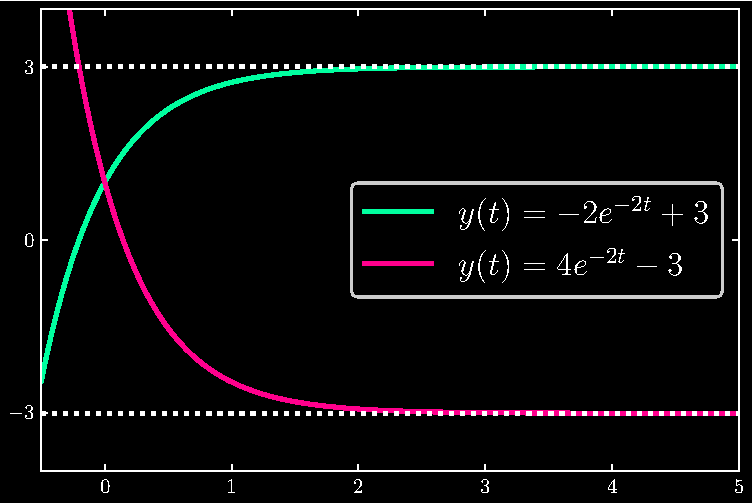
\includegraphics[width=1.0\textwidth]{chap1/sec1.4/chap1sec1.4ex11.eps}
\end{center}

% QUESTION 12
\qs{1.4.12}{Write the equations in Problem 11 as \(Y' = -2Y\) with \(Y = y - y_{\infty}\). What is \(Y \!\left( 0 \right) \)?}

By premise, \(Y = y - y_{\infty} = y - 3\) in the case of equation (a). Then \(Y' = y'\) and \(-2Y = -2 \!\left( y-3 \right) \). Then we may rewrite \(y' + 2y = 6\) as
\[
	\begin{aligned}
		Y' = y' &= -2y + 6  \\
		 & = -2 \!\left( y - 3 \right)  \\
		 & = -2 Y
	\end{aligned}
\]

Analogously, for equation (b), we have \(Y = y - y_{\infty} = y + 3\) and rewrite in form

\[
	\begin{aligned}
		Y' = y' &= -2y - 6  \\
		 &= -2 \!\left( y + 3 \right)  \\
		 &= -2Y
	\end{aligned}
\]

We define \(Y \!\left( 0 \right) = y \!\left( 0 \right) - y_{\infty}\). Since \(y \!\left( 0 \right) = 1\), in the case of (a), \(Y \!\left( 0 \right) = 1 - 3 = 2\), and for (b), \(Y \!\left( 0 \right) = 1 + 3 = 4\). Thus the rewritten forms of the equations are the same, albeit with differing initial conditions.

\vspace{12pt}

% QUESTION 13
\qs{1.4.13}{If a drip feeds \(q = 0.3\) grams per minute into your arm, and your body eliminates the drug at the rate \(6y\) grams per minute, what is the steady state concentration \(y_{\infty}\)? Then \(in = out\) and \(y_{\infty}\) is constant. Write a differential equation for \(Y = y - y_{\infty}\).}

By premise, \(y' = -6y\). Moreover, with a source \(q = 0.3\), we can conclude the differential equation before us is
\[
	y' = -6y + 0.3
\]

Assuming that the body begins with zero concentration of the drug (i.e. \(y \!\left( 0 \right) = 0\), we solve

\begin{alignat*}{3}
	&\implies && e^{6t} \!\left( y' + 6y \right)  && = 0.3 e^{6t} \\
	&\implies && \frac{d }{d t} \!\left( e^{6t}y \right)  && = 0.3 e^{6t} \\
	&\implies && e^{6t} y \!\left( t \right) && = 0.3 \int^{t}_{0} e^{6s} \ ds \\
	& && && = 0.05 \!\left( e^{6t} - 1 \right) \\
	&\implies && y \!\left( t \right) && = \underbrace{- 0.05 \!\left( e^{-6t} - 1 \right) }_{y_{p}} \\
	& && && = -0.05 e^{-6t} + 0.05
\end{alignat*}

Taking the limit gives us \(\lim\limits_{t \to \infty} y \!\left( t \right) = y_{\infty} = 0.05\). Thus the steady state drug mass in the bloodstream is \boxed{0.05 \text{ grams}}.

\begin{center}
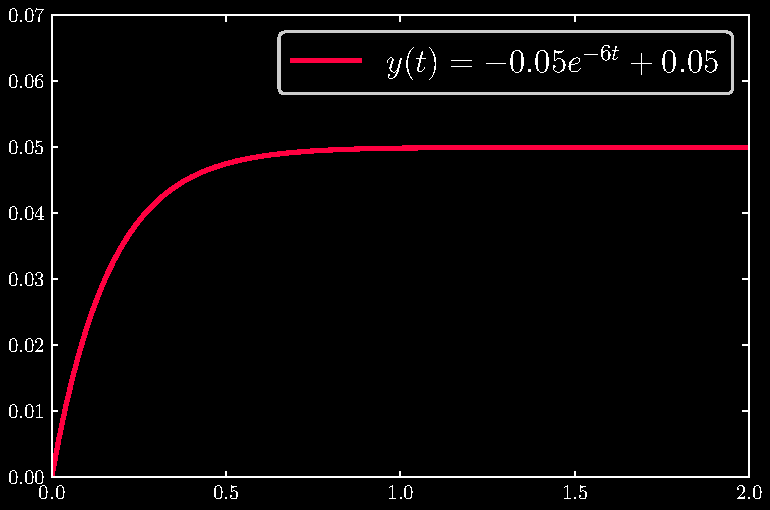
\includegraphics[width=1.0\textwidth]{chap1/sec1.4/chap1sec1.4ex13.eps}
\end{center}

Then we define \(Y = y - y_{\infty} = y - 0.05\), with \(Y' = y'\) and as such,
\begin{align*}
	Y' = y' & = -6y + 0.3 \\
	 & = -6 \!\left( y - 0.05 \right)  \\ 
	 & = -6 Y
\end{align*}

% QUESTION 14
\qs{1.4.14}{Why is \(y_{\infty}\) the same for \(y' + y = H \!\left( t-2 \right) \) and \(y' + y = H \!\left( t - 10 \right) \)?}

We begin with the first equation, which multiplied by integrating factor \(e^{t}\) yields:

\begin{alignat*}{3}
	&\implies && \!\left( e^{t} y \right)' && = e^{t} H \!\left( t - 2 \right)   \\
	&\implies && e^{t} y \!\left( t \right) - y \!\left( 0 \right) && = \int^{t}_{2} e^{s} \ ds   \\
	& && && = e^{t} - e^{2} \\
	&\implies && y \!\left( t \right) && = e^{-t} y \!\left( 0 \right) - \!\left( e^{2 - t} - 1 \right)
\end{alignat*}

Taking the limit as \(t \rightarrow \infty\), we find
\[
	\lim\limits_{t \to \infty} y \!\left( t \right) = 1
\]

Next, we find for the second equation, with integrating factor \(e^{t}\):

\begin{alignat*}{3}
	&\implies && \!\left( e^{t}y \right)' && = e^{t} H \!\left( t - 10 \right)  \\
	&\implies && e^{t} y \!\left( t \right) - y \!\left( 0 \right) && = \int^{t}_{10} e^{s} \ ds  \\ 
	&  && && = e^{t} - e^{10} \\
	&\implies && y \!\left( t \right) && = e^{-t} y \!\left( 0 \right) - \!\left( e^{10 - t} - 1 \right) 
\end{alignat*}

Analogously, we also find
\[
	\lim\limits_{t \to \infty} y \!\left( t \right)  = 1
\]
Intuitively, if we think of the Heaviside function as a switch, all that differs between the two equations is when we ``turn on" the switch to the source. The source itself has the same magnitude across the two equations, so there is no reason for the limiting behavior of \(y \!\left( t \right) \) to deviate from each other.

\begin{center}
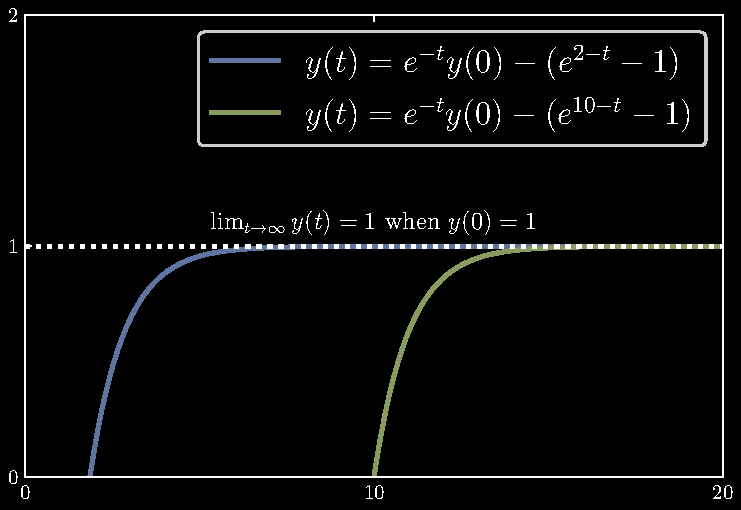
\includegraphics[width=1.0\textwidth]{chap1/sec1.4/chap1sec1.4ex14.eps}
\end{center}

% QUESTION 15
\qs{1.4.15}{Draw the ramp function that solves \(y' = H \!\left( t - T \right) \) with \(y \!\left( 0 \right) = 2\).}

We solve the equation by:

\begin{alignat*}{3}
	&\implies && \int^{t}_{0} \frac{d y}{d t}  \ dt && = \int^{t}_{T} H \!\left( t - T \right)  \ dt   \\
	&\implies && y \!\left( t \right) - y \!\left( 0 \right) && = R \!\left( t - T \right)  \\
	&\implies && y \!\left( t \right) && = 2 + R \!\left( t - T \right) 
\end{alignat*}

where we define \(R \!\left( t - T \right) \) as
\[
	R \!\left( t - T \right) = \begin{cases}
		t - T & t \ge T \\
		0 & t < T \\
	\end{cases}
\]

For \(T = 3\), we graph the solution as

\begin{center}
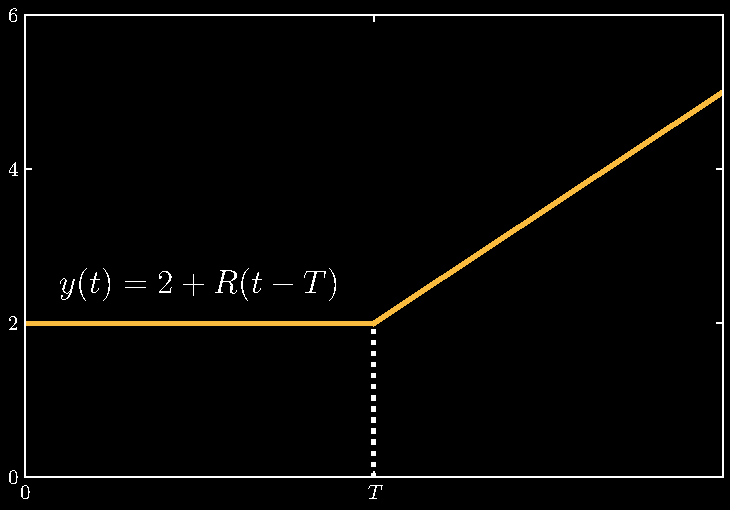
\includegraphics[width=1.0\textwidth]{chap1/sec1.4/chap1sec1.4ex15.eps}
\end{center}

% QUESTION 16
\qs{1.4.16}{Find \(y_{n} \!\left( t \right) \) and \(y_{p} \!\left( t \right) \) as in equation (10), with step function inputs starting at \(T = 4\).

\begin{enumerate}[label=(\alph*)]
	\item \(y' - 5y = 3H \!\left( t - 4 \right) \)
	\item \(y' + y = 7H \!\left( t - 4 \right) \)
\end{enumerate}

(\textit{What is \(y_{\infty}\)?})}

(a) Our integrating factor is \(e^{-5t}\). Solving the equation yields:

\begin{alignat*}{3}
	&\implies && \!\left( e^{-5t}y \right)' && = 3e^{-5t} H \!\left( t - 4 \right)  \\
	&\implies && e^{-5t} y \!\left( t \right) - y \!\left( 0 \right) && = \int^{t}_{4} 3e^{-5s} \ ds  \\
	& && && = -\frac{3}{5} \!\left( e^{-5t} - e^{-20} \right) \\
	&\implies && y \!\left( t \right) && = \underbrace{e^{5t} y \!\left( 0 \right)}_{y_{n} \!\left( t \right) } + \underbrace{\frac{3}{5} \!\left( e^{5 \!\left(t - 4 \right) } - 1 \right)}_{y_{p} \!\left( t \right) }
\end{alignat*}

Here, the asymptotic behavior of \(y \!\left( t \right) \) appears to diverge:
\[
	\lim\limits_{t \to \infty} y \!\left( t \right) = +\infty
\]

which we expect since the growth rate, \(a = 5\), is positive.

\begin{center}
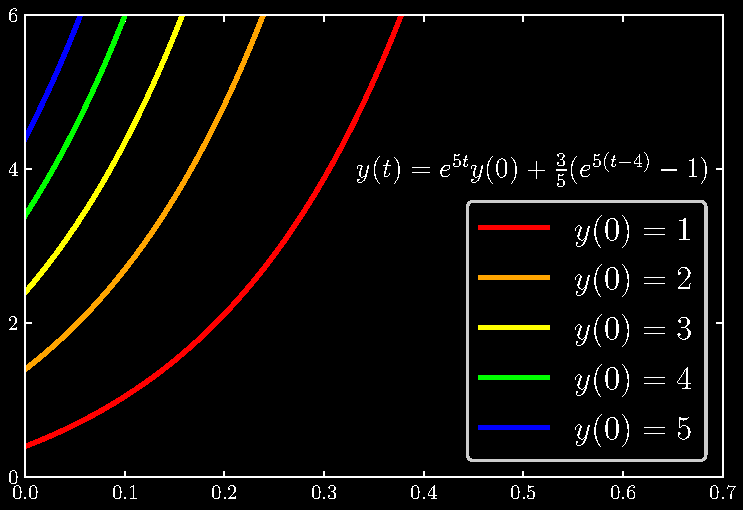
\includegraphics[width=1.0\textwidth]{chap1/sec1.4/chap1sec1.4ex16a.eps}
\end{center}

\vspace{12pt}

(b) Next, our integrating factor is \(e^{t}\):

\begin{alignat*}{3}
	&\implies && \!\left( e^{t}y \right)' && = 7 e^{t} H \!\left( t - 4 \right)  \\
	&\implies && e^{t} y \!\left( t \right) - y \!\left( 0 \right) && = \int^{t}_{4} 7e^{s} \ ds  \\
	& && && = 7 \!\left( e^{t} - e^{4} \right) \\
	&\implies && y \!\left( t \right) && = \underbrace{e^{-t} y \!\left( 0 \right)}_{y_{n} \!\left( t \right) } \underbrace{- 7 \!\left( e^{- \!\left( t - 4 \right) } - 1 \right)}_{y_{p} \!\left( t \right) }
\end{alignat*}

with limiting behavior
\[
	\lim\limits_{t \to \infty} y \!\left( t \right) = 7
\]

\begin{center}
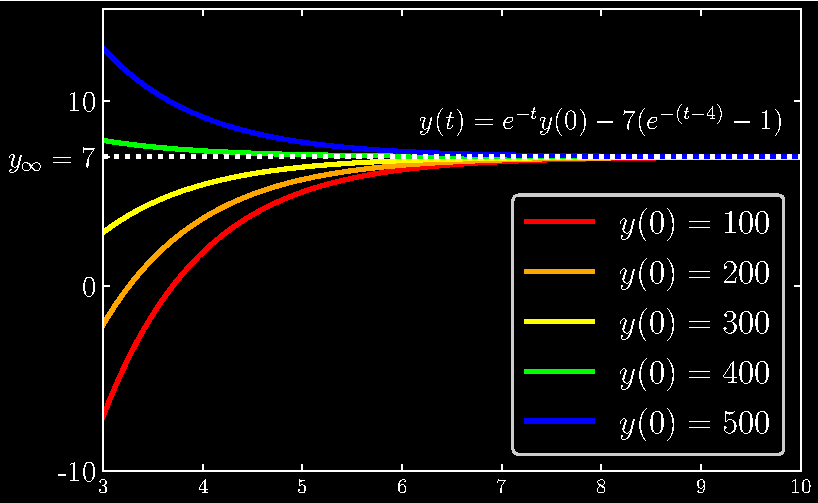
\includegraphics[width=1.0\textwidth]{chap1/sec1.4/chap1sec1.4ex16b.eps}
\end{center}

% QUESTION 17
\qs{1.4.17}{Suppose the step function turns on at \(T = 4\) and off at \(T = 6\). Then \(q \!\left( t \right) = H \!\left( t - 4 \right) - H \!\left( t - 6 \right) \). Starting from \(y \!\left( 0 \right) = 0\), solve \(y' + 2y = q \!\left( t \right) \). What is \(y_{\infty}\)?}

With integrating factor \(e^{2t}\), we derive:

\begin{alignat*}{3}
	&\implies && \!\left( e^{2t} y \right)' && = e^{2t} \left[ H \!\left( t-4 \right) - H \!\left( t-6 \right)  \right]  \\
	&\implies && e^{2t} y \!\left( t \right) && = \int^{t}_{4} e^{2s} \ ds - \int^{t}_{6} e^{2s} \ ds   \\ 
	& && && = \begin{cases}
		0 & 0 \le t < 4 \\
		\frac{1}{2} \!\left( e^{2t} - e^{8} \right) & 4 \le t < 6 \\
		\frac{1}{2} \!\left( e^{2t} - e^{8} \right) - \frac{1}{2} \!\left( e^{2t} - e^{12} \right) & 6 \le t 
	\end{cases}\\
	& && && = \begin{cases}
		0 & 0 \le t < 4 \\
		\frac{1}{2} \!\left( e^{2t} - e^{8} \right) & 4 \le t < 6 \\
		\frac{1}{2} \!\left( e^{12} - e^{8} \right) & 6 \le t 
	\end{cases} \\
	&\implies && y \!\left( t \right) && = \begin{cases}
		0 & 0 \le t < 4 \\
		-\frac{1}{2} \!\left( e^{-2 \!\left( t - 4 \right) } - 1\right) & 4 \le t < 6 \\
		-\frac{1}{2} \!\left( e^{-2 \!\left( t - 4 \right) }  - e^{-2 \!\left( t-6 \right) } \right) & 6 \le t
	\end{cases}
\end{alignat*}

More concisely, we may also write:
\[
	y \!\left( t \right) = \frac{1}{2} \left[ - \!\left( e^{-2 \!\left( t - 4 \right) } - 1 \right) H \!\left( t - 4 \right) + \!\left( e^{-2 \!\left( t - 6 \right) } - 1 \right) H \!\left( t - 6 \right)  \right] 
\]
Implying that
\[
	\lim\limits_{t \to \infty} y \!\left( t \right) = 0
\]

\begin{center}
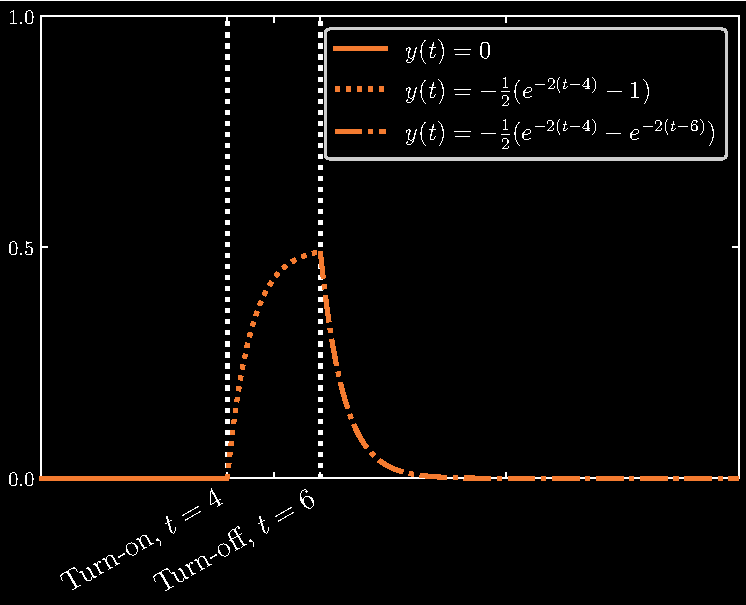
\includegraphics[width=1.0\textwidth]{chap1/sec1.4/chap1sec1.4ex17.eps}
\end{center}

% QUESTION 18
\qs{1.4.18}{Suppose \(y' = H \!\left( t-1 \right) + H \!\left( t-2 \right) + H \!\left( t-3 \right) \), starting at \(y \!\left( 0 \right) = 0\). Find \(y \!\left( t \right) \).}

Integrating yields
\[
	y = R \!\left( t - 1 \right) + R \!\left( t - 2 \right) + R \!\left( t - 3 \right) 
\]
but we may simplify this result further. Recall that the definition of our ramp function \(R \!\left( t - T\right) \) is
\[
	R \!\left( t - T \right) = \begin{cases}
		t - T & t \ge T \\
		0 & t < T \\
	\end{cases}
\]
Applying this to the constituent ramp functions of \(y \!\left( t \right) \), we can derive
\[
	y \!\left( t \right) = \begin{cases}
		0 & 0 \le t < 1 \\
		t - 1 & 1 \le t < 2 \\
		2t - 3 & 2 \le t < 3 \\
		3 \!\left( t - 2 \right) & 3 \ge t
	\end{cases}
\]
which alternatively can be written as
\[
	y \!\left( t \right) = \!\left( t - 1 \right) H \!\left( t - 1 \right) + \!\left( t - 2 \right) H \!\left( t - 2 \right) + \!\left( t - 3 \right) H \!\left( t - 3 \right) 
\]
Graphing the function, we can visually see what is happening here: as we turn on more and more switches (at times \(t = 1, 2, 3\) to more and more sources, the growth of \(y \!\left( t \right) \) happens at a steeper and steeper rate.

\begin{center}
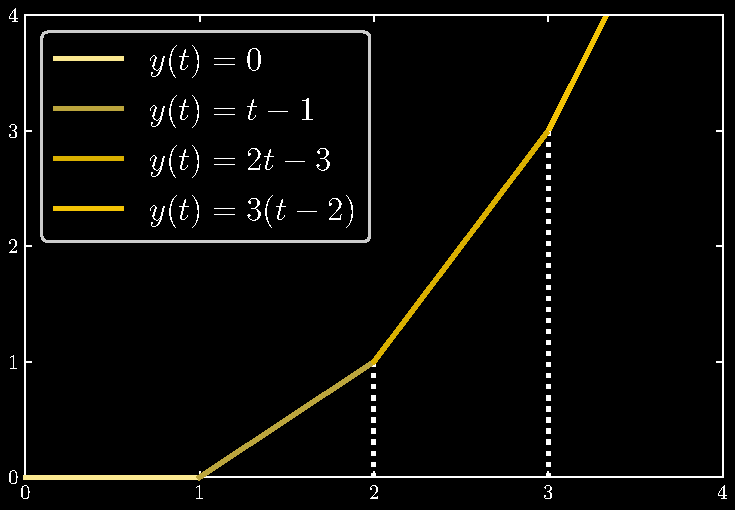
\includegraphics[width=1.0\textwidth]{chap1/sec1.4/chap1sec1.4ex18.eps}
\end{center}

% QUESTION 19
\qs{1.4.19}{For all \(t > 0\) find these integrals \(a \!\left( t \right) , b \!\left( t \right), c \!\left( t \right) \) of point sources and graph \(b \!\left( t \right) \):
\begin{enumerate}[label=(\alph*)]
	\item \( {\displaystyle \int^{t}_{0} \delta \!\left( T - 2 \right) \, dT} \)
	\item \({\displaystyle \int^{t}_{0} \!\left( \delta \!\left( T - 2 \right) - \delta \!\left( T - 3 \right) \right)  \, dT} \)
	\item \( {\displaystyle \int^{t}_{0} \delta \!\left( T - 2 \right) \delta \!\left( T - 3 \right)  \, dT} \)
\end{enumerate}}

(a) If \(t \ge 2\), it will be the case that the domain of integration includes the point \(T = 2\). Ergo, we have
\[
	a \!\left( t \right) = \int^{t}_{0} \delta \!\left( T - 2 \right)  \, dT = H \!\left( T - 2 \right) = \begin{cases}
		0 & t < 2 \\
		1 & t \ge 2 \\
	\end{cases}
\]
Graphically, we have
\begin{center}
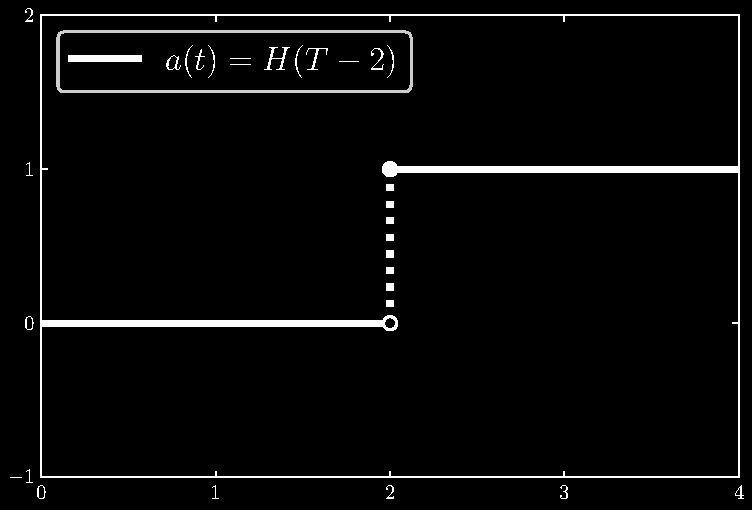
\includegraphics[width=1.0\textwidth]{chap1/sec1.4/chap1sec1.4ex19a.eps}
\end{center}
(b) We rewrite \(b \!\left( t \right) \) as
\[
	b \!\left( t \right) = \int^{t}_{0} \!\left( \delta \!\left( T - 2 \right) - \delta \!\left( T - 3 \right)  \right)  \, dT = \int^{t}_{0} \delta \!\left( T - 2 \right)  \, dT - \int^{t}_{0} \delta \!\left( T - 3 \right)  \, dT   
\]
Now, the value of each term is contingent on our choice of \(t\). For \(t < 2\), each term vanishes. For \(2 \le t < 3\), the first term is 1, while the second term vanishes. Lastly, for \(t \ge 3\), both terms are 1, and the difference vanishes. Succinctly, put, we have 
\[
	\int^{t}_{0} \delta \!\left( T-2 \right)  \, dT = H \!\left( T-2 \right) \qquad \text{and} \qquad \int^{t}_{0} \delta \!\left( T-3 \right)  \, dT = H \!\left( T-3 \right)   
\]
and solve as
\[
	b \!\left( t \right) = \int^{t}_{0} \!\left( \delta \!\left( T - 2 \right) - \delta \!\left( T - 3 \right)  \right)  \, dT = \begin{cases}
		1 & 2 \le t < 3 \\
		0 & \text{otherwise} \\
	\end{cases} 
\]

Intuitively, we can interpret this as at time \(T = 2\), we ``deposit" an impulse, and at time \(T = 3\), we ``withdraw" the impulse, leaving us with nothing once more. Graphically, we represent \(b \!\left( t \right) \) as

\begin{center}
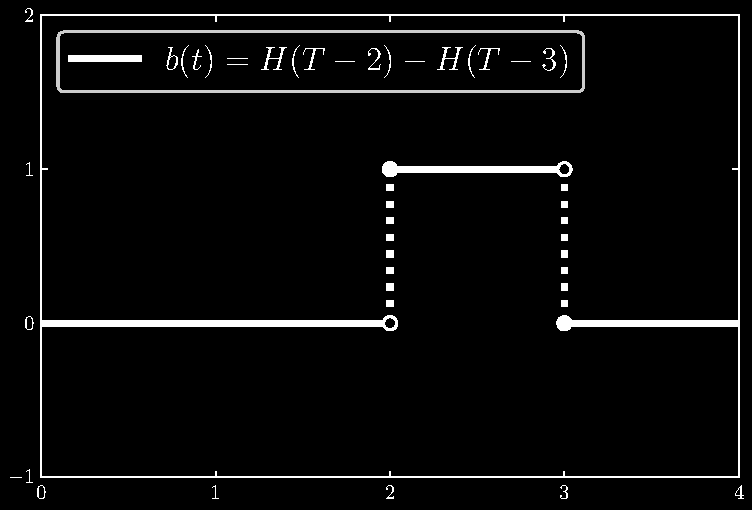
\includegraphics[width=1.0\textwidth]{chap1/sec1.4/chap1sec1.4ex19bi.eps}
\end{center}

along with the integrand

\begin{center}
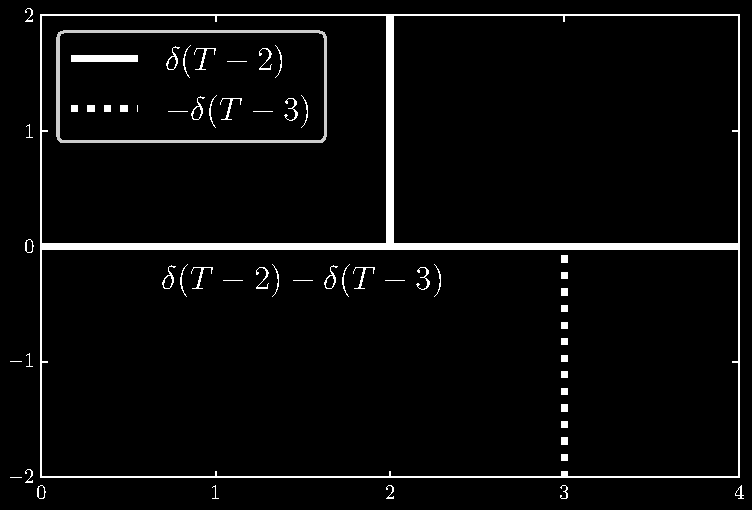
\includegraphics[width=1.0\textwidth]{chap1/sec1.4/chap1sec1.4ex19b.eps}
\end{center}

(c) Observe that irrespective of our choice of \(t\), it cannot ever be the case that the product \(\delta \!\left( T - 2 \right) \delta \!\left( T - 3 \right) \) is equal to anything other than zero. For when either constituent of the product is non-zero, it must be the case that the other is zero. Conceptually, we may have an impulse at one time for one of the delta functions, but that means there cannot be an impulse in the other delta function. Hence,
\[
	c \!\left( t \right) = \int^{t}_{0} \delta \!\left( T - 2 \right) \delta \!\left( T - 3 \right)  \, dT = 0 \text{ for all } t 
\]

% QUESTION 20
\qs{1.4.20}{Why are all these answers reasonable? (They are all correct.)
\begin{enumerate}[label=(\alph*)]
	\item \( \displaystyle \int^{\infty}_{-\infty} e^{t} \delta \!\left( t \right)  \, dt = 1\)
	\item \( \displaystyle \int^{\infty}_{-\infty} \!\left( \delta \!\left( t \right)  \right)^{2}  \, dt = \infty \)
	\item \( \displaystyle \int^{\infty}_{-\infty} e^{T}\delta \!\left( t - T \right)  \, dT = e^{t} \)
\end{enumerate}}

(a) Recall that
\[
	\int^{\infty}_{-\infty} \delta \!\left( t \right) F \!\left( t \right)  \, dt = F \!\left( 0 \right)  
\]
Therefore, we have \(F \!\left( t \right) = e^{t}\), thus
\[
	\int^{\infty}_{-\infty} e^{t} \delta \!\left( t \right)  \, dt = e^{0} = 1
\]

(b) Again invoking the aforementioned identity, we have \(F \!\left( t \right) = \delta \!\left( t \right) \), giving us
\[
	\int^{\infty}_{-\infty} \!\left( \delta \!\left( t \right)  \right)^{2} \, dt = \delta \!\left( 0 \right) = \infty 
\]

(c) Here we recall the identity
\[
	\int^{\infty}_{-\infty} \delta \!\left( t - T \right) F \!\left( t \right)  \, dt = F \!\left( T \right)  
\]
In the given integral equation, however, the variable of integration is \(T\). What matters is the value that \(F \!\left( T \right) = e^{T}\) takes is time \(T\) at which \(\delta \!\left( t - T \right) \) has argument zero. This is precisely when \(T = t\), hence
\[
	\int^{\infty}_{-\infty} e^{T} \delta \!\left( t - T \right)  \, dT = e^{t}
\]

% QUESTION 21
\qs{1.4.21}{\textit{The solution to} \(y' = 2y + \delta \!\left( t - 3 \right) \) \textit{jumps up by } \(1\) \textit{at} \(t = 3\). Before and after \(t = 3\), the delta function is zero and \(y\) grows like \(e^{2t}\). Draw the graph of \(y \!\left( t \right) \) when
\begin{enumerate}[label=(\alph*)]
	\item \( y \!\left( 0 \right) = 0 \) and
	\item \(y \!\left( 0 \right) = 1\).
\end{enumerate}
Write formulas for \(y \!\left( t \right) \) before and after \(t = 3\).}

We solve the differential equation with integrating factor \(e^{-2t}\) as follows:

\begin{alignat*}{3}
	&\implies && y' - 2y && = \delta \!\left( t - 3 \right)  \\
	&\implies && \!\left( e^{-2t}y \right)' && = e^{-2t} \delta \!\left( t - 3 \right)  \\
	&\implies && e^{-2t}y \!\left( t \right) - y \!\left( 0 \right) && = \int^{t}_{0} e^{-2s} \delta \!\left( s-3 \right)  \, ds \\
	& && && = \begin{cases}
		0 & 0 \le t < 3 \\
		\displaystyle{e^{-6}} & t \ge 3 
		\end{cases} \\
	&\implies && y \!\left( t \right) && = \begin{cases}
		e^{2t} y \!\left( 0 \right)  & 0 \le t < 3 \\
		\displaystyle{e^{2t} y \!\left( 0 \right) + e^{2 \!\left( t - 3 \right) }} & t \ge 3 
		\end{cases} \\
										       & && && = e^{2t} y \!\left( 0 \right) + H \!\left( t - 3 \right) e^{2 \!\left( t - 3 \right) }
\end{alignat*}

In the case of (a), we have
\[
	y \!\left( t \right) = H \!\left( t - 3 \right) e^{2 \!\left( t-3 \right) }
\]
and for (b)
\[
	y \!\left( t \right) = e^{2t} + H \!\left( t - 3 \right) e^{2 \!\left( t - 3 \right) }
\]
which has graph
\begin{center}
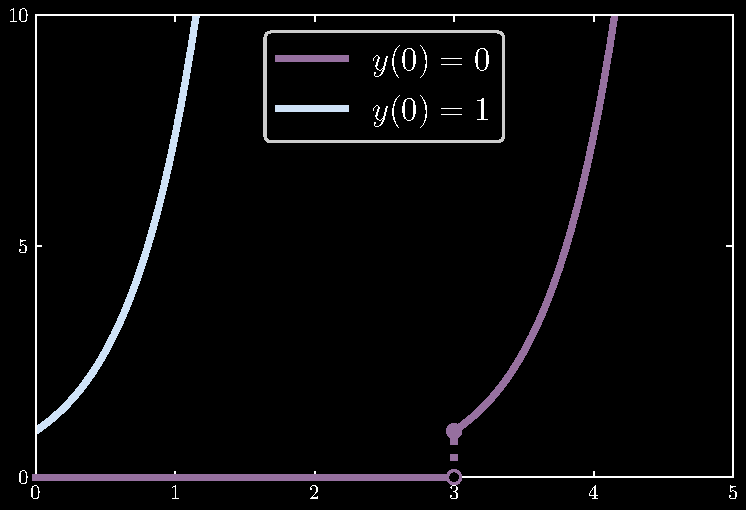
\includegraphics[width=1.0\textwidth]{chap1/sec1.4/chap1sec1.4ex21.eps}
\end{center}

% QUESTION 22
\qs{1.4.22}{Solve these differential equations starting at \(y \!\left( 0 \right) = 2\):
\begin{enumerate}[label=(\alph*)]
	\item \(y' - y = \delta \!\left( t - 2 \right) \)
	\item \(y' + y = \delta \!\left( t - 2 \right) \)
\end{enumerate}
(\textit{What is \(y_{\infty}\)}?)}

(a) Beginning with integrating factor \(e^{-t}\), we have
\begin{alignat*}{3}
	&\implies && \!\left( e^{-t} y \right)' && = e^{-t} \delta \!\left( t - 2 \right)  \\
	&\implies && e^{-t} y \!\left( t \right) - y \!\left( 0 \right) && = \int^{t}_{0} e^{-s} \delta \!\left( s-2 \right)  \, ds  \\
	& && && = \begin{cases}
		0 & 0 \le t < 2 \\
		e^{-2} & t \ge 2 \\
	\end{cases} \\
	&\implies && y \!\left( t \right) && = e^{t} y \!\left( 0 \right) + H \!\left( t - 2 \right) e^{t-2} \\
	& && && = 2e^{t} + H \!\left( t - 2 \right) e^{t-2}
\end{alignat*}
It follows that
\[
	\lim\limits_{t \to \infty} y \!\left( t \right) = +\infty
\]
(b) Now, with integrating factor \(e^{t}\), we have
\begin{alignat*}{3}
	&\implies && \!\left( e^{t}y \right)' && = e^{t} \delta \!\left( t-2 \right)  \\
	&\implies && e^{t} y \!\left( t \right) - y \!\left( 0 \right) && = \int^{t}_{0} e^{s} \delta \!\left( s - 2 \right)  \, ds  \\ 
	& && && = \begin{cases}
		0 & 0 \le t < 2 \\
		e^{2} & t \ge 2 \\
	\end{cases} \\
	&\implies && y \!\left( t \right) && = e^{-t} y \!\left( 0 \right) + H \!\left( t-2 \right) e^{-\!\left( t-2 \right) } \\
	& && && = 2 e^{-t} + H \!\left( t - 2 \right) e^{-\!\left( t-2 \right) }
\end{alignat*}
which has limiting behavior
\[
	\lim\limits_{t \to \infty} = 0
\]

Intuitively, in the case of (b), we have an instantaneous impulse at time \(t=2\), after which we have a decay.

\begin{center}
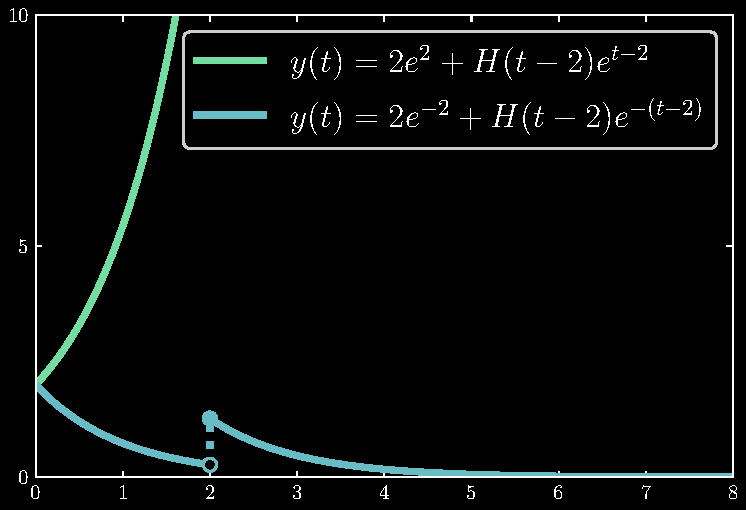
\includegraphics[width=1.0\textwidth]{chap1/sec1.4/chap1sec1.4ex22.eps}
\end{center}

% QUESTION 23
\qs{1.4.23}{Solve \(dy/dt = H \!\left( t-1 \right) + \delta \!\left( t-1 \right) \) starting from \(y \!\left( 0 \right) = 0\): jump and ramp.}

Solving as follows, we find
\begin{alignat*}{3}
	&\implies && y \!\left( t \right) - y \!\left( 0 \right) && = \int^{t}_{0} H \!\left( s-1 \right)  \, ds + \int^{t}_{0} \delta \!\left( s-1 \right)  \, ds   \\
	&\implies && y \!\left( t \right) && = R \!\left( t-1 \right) + H \!\left( t - 1 \right)   \\
	& && && = \begin{cases}
		0 & t < 1 \\
		t & t \ge 1 \\
	\end{cases}
\end{alignat*}

Intuitively, at time \(t=1\), we have an impulse which causes a jump to \(y \!\left( 1 \right) = 1\), after which we have constant growth through the ramp function.
\begin{center}
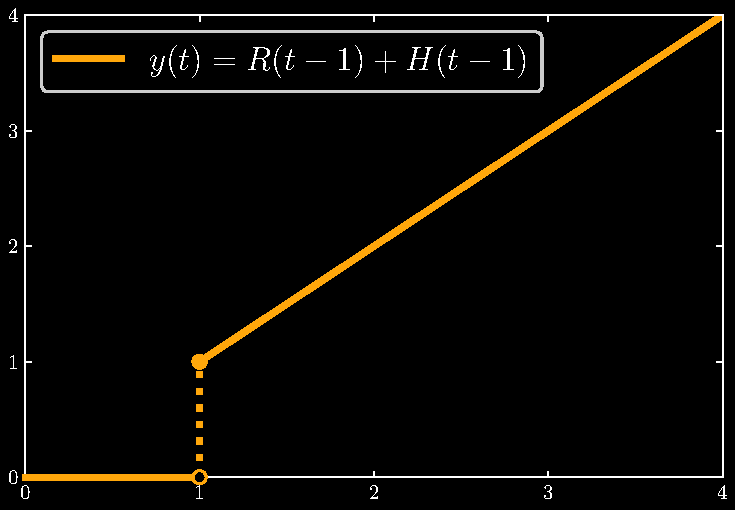
\includegraphics[width=1.0\textwidth]{chap1/sec1.4/chap1sec1.4ex23.eps}
\end{center}

% QUESTION 24
\qs{1.4.24}{(My small favorite) What is the steady state \(y_{\infty}\) for \(y' = -y + \delta \!\left( t-1 \right) + H 
\!\left( t-3 \right) \)?}
Using integrating factor \(e^{t}\), we find
\begin{alignat*}{3}
	&\implies && y' + y && = \delta \!\left( t-1 \right) + H \!\left( t-3 \right)  \\
	&\implies && \!\left( e^{t}y \right)' && = e^{t} \delta \!\left( t-1 \right) + e^{t} H \!\left( t-3 \right)  \\ 
	&\implies && e^{t} y \!\left( t \right) - y \!\left( 0 \right) && = \int^{t}_{0} e^{s} \delta \!\left( s-1 \right)  \, ds + \int^{t}_{0} e^{s} H \!\left( s-3 \right)  \, ds \\
	& && && = e H \!\left( t-1 \right) + e^{t} H \!\left( t-3 \right) \\
	&\implies && y \!\left( t \right) && = e^{-t} y \!\left( 0 \right) + e^{-\!\left( t-1 \right) } H \!\left( t-1 \right) + H \!\left( t-3 \right) 
\end{alignat*}
which features limiting behavior
\[
	\lim\limits_{t \to \infty} y \!\left( t \right) = 1
\]
Thus our steady state is \(y_{\infty} = 1\).

\vspace{12pt}

% QUESTION 25
\qs{1.4.25}{Which \(q\) and \(y \!\left( 0 \right) \) in \(y' - 3y = q \!\left( t \right) \) produce the step solution \(y \!\left( t \right) = H \!\left( t-1 \right) \)?}

Given \(y \!\left( t \right) = H \!\left( t-1 \right) \), we must have \(y \!\left( 0 \right) = 0\). Moreover, it follows that \(y'\!\left( t \right) = \delta \!\left( t-1 \right) \). Thus \(q \!\left( t \right) \) must be
\[
	q \!\left( t \right) = \delta \!\left( t-1 \right) - 3 H \!\left( t-1 \right) 
\]
Graphically, the source \(q \!\left( t \right) \) appears as
\begin{center}
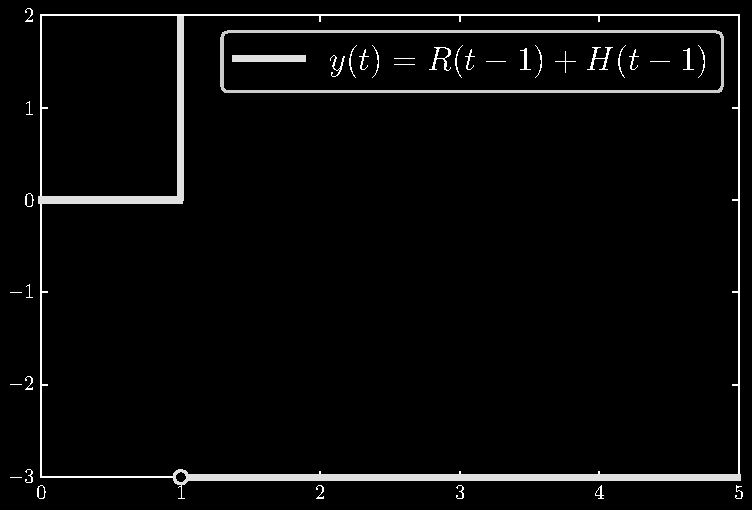
\includegraphics[width=1.0\textwidth]{chap1/sec1.4/chap1sec1.4ex25.eps}
\end{center}

% QUESTION 26
\qs{1.4.26}{Solve these equations \(y' - ay = Qe^{ct}\) as in (19), starting from \(y \!\left( 0 \right) = 2\):
\begin{enumerate}[label=(\alph*)]
	\item \(y' - y = 8e^{3t}\)
	\item \(y' + y = 8e^{-3t}\)
\end{enumerate}
(\textit{What is} \(y_{\infty}\)?)}

(a) Let \(y_{p} = 8Ye^{3t}\). Then \(y_{p}' = 24Ye^{3t}\) and we have, substituting \(y_{p}\) for \(y\):
\begin{alignat*}{3}
	&\implies && 24Ye^{3t} - 8Ye^{3t} && = 8e^{3t} \\
	&\implies && 3Y - Y && = 1 \\ 
	&\implies && Y && = 1/2
\end{alignat*}
Thus we have that \(y_{p} = 4e^{3t}\), where the particular solution starts at \(y_{p} \!\left( 0 \right) = 4\). The null solution must start at \(-2\), and is given by
\[
	y_{n} = -2e^{t}
\]
And the complete solution is
\[
	y \!\left( t \right) = \underbrace{-2e^{t}}_{y_{n}} + \underbrace{4e^{3t}}_{y_{p}}
\]
with limiting behavior
\[
	\lim\limits_{t \to \infty} y \!\left( t \right) = +\infty
\]
(b) Let \(y_{p} = 8Ye^{-3t}\). Then \(y_{p}' = -24Ye^{-3t}\) and we have, substituting \(y_{p}\) for \(y\):
\begin{alignat*}{3}
	&\implies && -24Ye^{-3t} + 8Ye^{-3t} && = 8e^{-3t} \\
	&\implies && -3Y + Y && = 1 \\
	&\implies && Y && = -1/2
\end{alignat*}
So we must have \(y_{p} = -4e^{-3t}\). As our particular solution begins at \(y_{p} \!\left( 0 \right) = -4\), our null solution must commence at 6, giving us
\[
	y_{n} = 6e^{-t}
\]
Thus we have complete solution
\[
	y \!\left( t \right) = \underbrace{6e^{-t}}_{y_{n}} \underbrace{-4e^{-3t}}_{y_{p}}
\]
with limiting behavior
\[
	\lim\limits_{t \to \infty} y \!\left( t \right) = 0
\]
\begin{center}
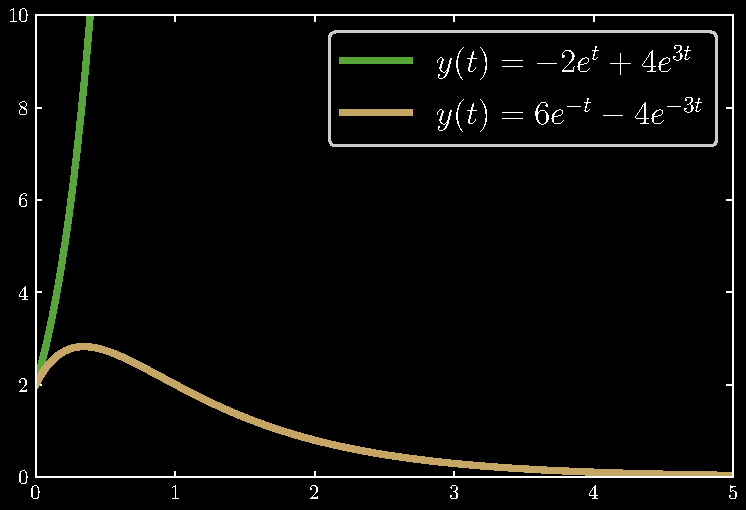
\includegraphics[width=1.0\textwidth]{chap1/sec1.4/chap1sec1.4ex26.eps}
\end{center}

% QUESTION 27
\qs{1.4.27}{When \(c = 2.01\) is very close to \(a = 2\), solve \(y' - 2y = e^{ct}\) starting from \(y \!\left( 0 \right) = 1\). This is resonance as in equation (20). By hand or computer, draw the graph of \(y \!\left( t \right) \).}

Let \(y_{p} = Ye^{ct}\). Then \(y_{p}' = cYe^{ct}\), and substituting, we find
\begin{alignat*}{3}
	&\implies && cYe^{ct} - 2Ye^{ct} && = e^{ct} \\
	&\implies && cY - 2Y = 1 \\ 
	&\implies && Y = \frac{1}{c - 2}
\end{alignat*}
Thus
\[
	y_{p} = \frac{e^{ct}}{c - 2}
\]
which starts at \(y_{p} \!\left( 0 \right) = \displaystyle{\frac{1}{c-2}}\). Then \(y_{n}\) must begin at \(\displaystyle{\frac{c - 3}{c - 2}}\), giving us
\[
	y_{n} = \frac{c-3}{c-2} e^{2t}
\]
and finally, the complete solution
\[
	y \!\left( t \right) = \underbrace{\frac{c-3}{c-2} e^{2t}}_{y_{n}} + \underbrace{\frac{1}{c-2} e^{ct}}_{y_{p}}
\]
For \(c = 2.01\), we evaluate \(y \!\left( t \right) \) as
\[
	y \!\left( t \right) = \underbrace{-99e^{2t}}_{y_{n}} + \underbrace{100e^{2.01t}}_{y_{p}}
\]
Cycling through values of \(c\) as we approach 2, we can graph the following trajectories:
\begin{center}
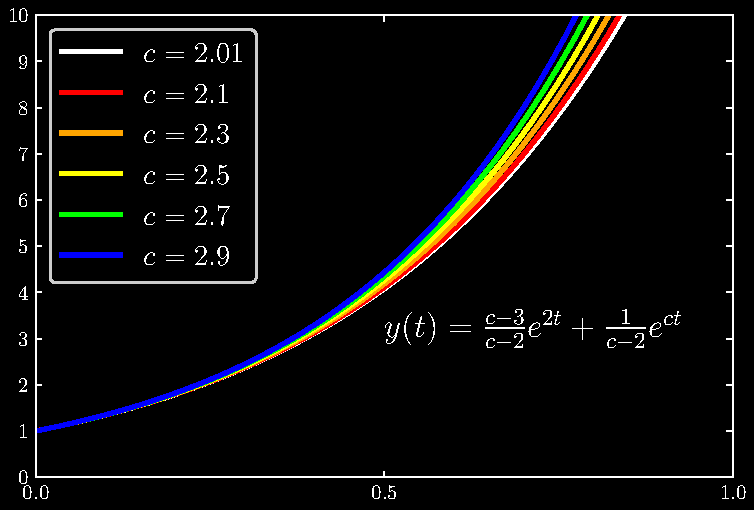
\includegraphics[width=1.0\textwidth]{chap1/sec1.4/chap1sec1.4ex27.eps}
\end{center}

% QUESTION 28
\qs{1.4.28}{When \(c = 2\) is exactly equal to \(a = 2\), solve \(y' - 2y = e^{2t}\) starting from \(y \!\left( 0 \right) = 1\). This resonance is as in equation (20). By hand or computer, draw the graph of \(y \!\left( t \right) \).}

Using the integrating factor \(e^{-2t}\), write
\begin{alignat*}{3}
	&\implies && \!\left( e^{-2t}y \right)' && = 1 \\
	&\implies && e^{-2t}y \!\left( t \right) - y \!\left( 0 \right) && = \int^{t}_{0} \, ds  \\ 
	&\implies && y \!\left( t \right) && = \underbrace{e^{2t}}_{y_{n}} + \underbrace{te^{2t}}_{y_{p}}
\end{alignat*}

We graphically represent \(y \!\left( t \right) \) as:
\begin{center}
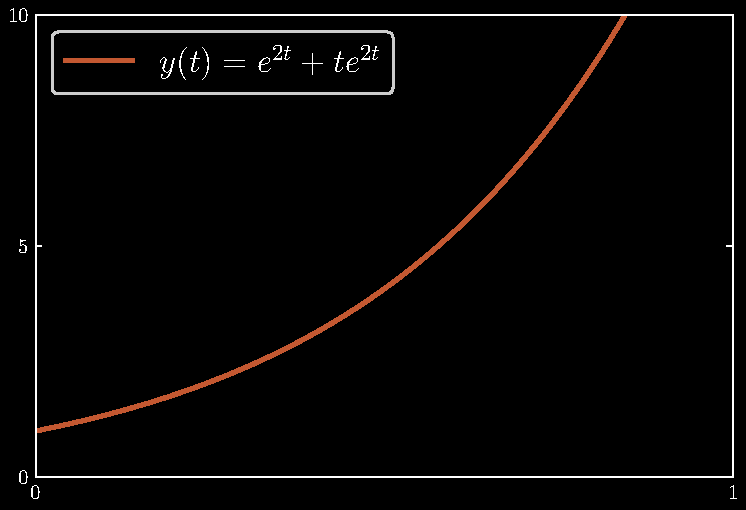
\includegraphics[width=1.0\textwidth]{chap1/sec1.4/chap1sec1.4ex28.eps}
\end{center}

% QUESTION 29
\qs{1.4.29}{Solve \(y' + 4y = 8e^{-4t} + 20\) starting from \(y \!\left( 0 \right) = 0\). What is \(y_{\infty}\)?}

Using integrating factor \(e^{4t}\), we have
\begin{alignat*}{3}
	&\implies && \!\left( e^{4t}y \right)' && = 8 + 20e^{4t}\\
	&\implies && e^{4t} y \!\left( t \right) - y \!\left( 0 \right) && = \int^{t}_{0} 8 \, ds + \int^{t}_{0} 20e^{4s} \, ds   \\
	&\implies && y \!\left( t \right) && = e^{-4t} y \!\left( 0 \right) + 8te^{-4t} - 5e^{-4t} + 5 \\
	& && && = 5 - 5e^{-4t} + 8te^{-4t}
\end{alignat*}

which has limiting behavior
\[
	\lim\limits_{t \to \infty} y \!\left( t \right) = 5
\]

% QUESTION 30
\qs{1.4.30}{The solution to \(y' - ay = e^{ct}\) didn't come from the main formula (4), but it could. Integrate \(e^{-as}e^{cs}\) in (4) to reach the very particular solution \(\!\left( e^{ct} - e^{at} \right) / \!\left( c - a \right) \).}

Using the integrating factor \(e^{-at}\), derive
\begin{alignat*}{3}
	&\implies && \!\left( e^{-at}y \right)' && = e^{-at} e^{ct} \\
	&\implies && e^{-at} y \!\left( t \right) - y \!\left( 0 \right) && = \int^{t}_{0} e^{\!\left( c - a \right) s} \, ds   \\ 
	& && && = \frac{e^{\!\left( c - a \right) t} - 1}{c - a} \\
	&\implies && y \!\left( t \right) && = e^{at} y \!\left( 0 \right) + \frac{e^{ct} - e^{at}}{c - a}
\end{alignat*}
where the second term is the very particular solution.

% QUESTION 31
\qs{1.4.31}{\textit{The easiest possible equation} \(y' = 1\) \textit{has resonance}! The solution \(y = t\) shows the factor \(t\). What number is the growth rate \(a\) and also the exponent \(c\) in the source?}

Here, we have \(a = c = 0\); it is clear that \(y' - ay = e^{ct}\) reduces to \(y' = 1\) with the aforementioned values.

\vspace{12pt}

% QUESTION 32
\qs{1.4.32}{Suppose you know two solutions \(y_{1}\) and \(y_{2}\) to the equation \(y' - a \!\left( t \right) y = q \!\left( t \right) \).
\begin{enumerate}[label=(\alph*)]
	\item Find a null solution to \(y' - a \!\left( t \right) y = 0\).
	\item Find all null solutions \(y_{n}\). Find all particular solutions \(y_{p}\).
\end{enumerate}}

(a) By premise, \(y_{1}\) and \(y_{2}\) solve the differential equation, meaning
\[
	y_{1}' - a \!\left( t \right) y_{1} = q \!\left( t \right) \qquad \text{and} \qquad y_{2}' - a \!\left( t \right) y_{2} = q \!\left( t \right) 
\]
In appealing to linearity, we can immediately deduce that the differences of the solutions, \(y_{1} - y_{2}\) and \(y_{2} - y_{1}\), are both null solutions:
\[
	\!\left( y_{1} - y_{2} \right)' - a \!\left( t \right) \!\left( y_{1} - y_{2} \right) = 0 \qquad \text{and} \qquad \!\left( y_{2} - y_{1} \right)' - a \!\left( t \right) \!\left( y_{2} - y_{1} \right) = 0
\]
(b) Once again appealing to linearity, all null solutions include solutions of the form \(\alpha \!\left( y_{1} - y_{2} \right)\) for all \(\alpha \in \mathbb{R}\). Moreover, observe that if we have \(\alpha y_{1}\) and \(\beta y_{2}\), we have
\[
	\alpha \!\left( y_{1}' - a \!\left( t \right) y_{1}\right) = \alpha q \!\left( t \right) \qquad \text{and} \qquad \beta \!\left( y_{2}' - a \!\left( t \right) y_{2} \right) = \beta q \!\left( t \right)  
\]
Then for any nonzero sum \(\alpha + \beta \), \(\alpha, \beta \in \mathbb{R}\), we have a ``weighted average" \textbf{linear combination} of particular solutions:
\[
	\frac{\alpha }{\alpha + \beta } y_{1} + \frac{\beta }{\alpha + \beta } y_{2}
\]

% QUESTION 33
\qs{1.4.33}{Turn back to the first page of this Section 1.4. Without looking, can you write down a solution to \(y' - ay = q \!\left( t \right) \) for all four source functions \(\bm{q }, \bm{H \!\left( t \right) }, \bm{\delta \!\left( t \right) }, \bm{e^{ct}}\)?}

For simplicity, assume \(y \!\left( 0 \right) = 0\).

\(\bm{q}:\) \(y' - ay = q\)

Using integrating factor \(e^{-at}\), calculate
\begin{alignat*}{3}
	&\implies && \!\left( e^{-at}y \right)' && = e^{-at} q  \\
	&\implies && e^{-at} y \!\left( t \right) && = \int^{t}_{0} e^{-as}q  \, ds   \\ 
	& && && = -\frac{q }{a} \!\left( e^{-at} - 1 \right) \\ 
	&\implies && y \!\left( t \right) && = -\frac{q }{a} \!\left( 1 - e^{at} \right) \\
	& && && = \boxed{\frac{q }{a} \!\left( e^{at} - 1 \right) }
\end{alignat*}

\(\bm{H \!\left( t \right) }\): \(y' - ay = H \!\left( t \right) \)

Using integrating factor \(e^{-at}\), calculate
\begin{alignat*}{3}
	&\implies && \!\left( e^{-at}y \right)' && = e^{-at} H \!\left( t \right)   \\
	&\implies && e^{-at} y \!\left( t \right) && = \int^{t}_{0} e^{-as} H \!\left( s \right)  \, ds  \\ 
	& && && = -\frac{1}{a} \!\left( e^{-at} - 1 \right) \\
	&\implies && y \!\left( t \right) && = \boxed{ \frac{1}{a} \!\left( e^{at} - 1 \right) }
\end{alignat*}

\(\bm{\delta \!\left( t \right) }\): \(y' - ay = \delta \!\left( t \right) \)

Using integrating factor \(e^{-at}\), calculate
\begin{alignat*}{3}
	&\implies && \!\left( e^{-at}y \right)' && = e^{-at} \delta \!\left( t \right)  \\
	&\implies && e^{-at} y \!\left( t \right) && = \int^{t}_{0} e^{-as} \delta \!\left( s \right)  \, ds   \\ 
	& && && = 1 \\
	&\implies && y \!\left( t \right) && = \boxed{ e^{at} }
\end{alignat*}

\(\bm{e^{ct}}\): \(y' - ay = e^{ct}\)

Assume that \(a \neq c\). Using integrating factor \(e^{-at}\), calculate
\begin{alignat*}{3}
	&\implies && \!\left( e^{-at}y \right)' && = e^{-at} e^{ct} \\
	&\implies && e^{-at} y \!\left( t \right) && = \int^{t}_{0} e^{-as} e^{cs} \, ds   \\ 
	& && && = \frac{1}{c - a} \!\left( e^{\!\left( c - a \right) t}- 1 \right) \\
	&\implies && y \!\left( t \right) && = \boxed{\frac{e^{ct} - e^{at}}{c - a}}
\end{alignat*}

Now suppose that \(a = c\). Then we have \(y' - ay = e^{at}\), and derive with integrating factor \(e^{-at}\)
\begin{alignat*}{3}
	&\implies && \!\left( e^{-at}y \right)' && = e^{-at} e^{at} \\
	&\implies && e^{-at} y \!\left( t \right) && = \int^{t}_{0}  \, ds   \\
	&\implies && y \!\left( t \right) && = \boxed{ te^{at} }
\end{alignat*}

% QUESTION 34
\qs{1.4.34}{Three of those sources in Problem 33 are actually the same, if you choose the right values for \(q \) and \(c\) and \(y \!\left( 0 \right) \). What are those values?}

Let \(q = 1\), \(c = 0\), and \(y \!\left( 0 \right) = 0\). Then the sources \(q \), \(e^{ct}\), and \(H \!\left( t \right) \) are equivalent.

\vspace{12pt}

% QUESTION 35
\qs{1.4.35}{What differential equations \(y' = ay + q \!\left( t \right) \) would be solved by \(y_{1} \!\left( t \right) \) and \(y_{2} \!\left( t \right) \)? Jumps, ramps, corners -- maybe harder than expected.}
\begin{center}
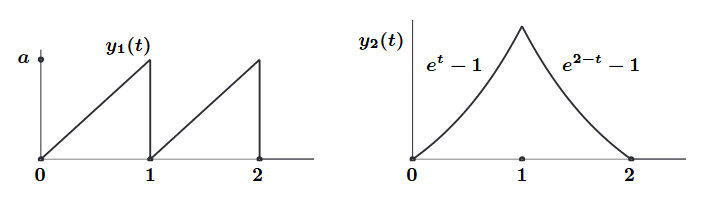
\includegraphics[width=1.0\textwidth]{chap1/sec1.4/ex35.png}
\end{center}
The equation for \(y_{1} \!\left( t \right) \) is
\[
	y_{1} \!\left( t \right) = a R \!\left( t \right) \!\left( 1 - H \!\left( t - 1 \right)  \right) + a R \!\left( t - 1\right) \!\left( 1 - H \!\left( t - 2 \right)  \right) 
\]
For \(y_{2} \!\left( t \right) \), we have
\[
	y_{2} \!\left( t \right) = \!\left( e^{t} - 1 \right) \!\left( 1 - H \!\left( t - 1 \right)  \right) + \!\left( e^{2 - t} - 1 \right) H \!\left( t - 1 \right) 
\]
In the case of \(y_{1} \!\left( t \right) \), differentiate to find
\begin{align*}
	y_{1}' & = a \left[ H \!\left( t \right) \!\left( 1 - H \!\left( t - 1 \right)  \right)  - R \!\left( t \right) \delta \!\left( t - 1 \right) \right] \\
	       & \quad + a \left[ H \!\left( t - 1 \right) \!\left( 1 - H \!\left( t - 2 \right)  \right)  - R \!\left( t - 1 \right) \delta \!\left( t - 2 \right) \right] 
\end{align*}
This is a complicated-looking expression, so we will go by interval and study the behavior of the derivative as \(t\) increases.

First, over \(0 \le t < 1\), we have \(y_{1}' = a\). At precisely \(t = 1\), however, the first delta function kicks in, plunging \(y_{1}'\) down to \(-\infty\) at that very instant. Moving over \(1 < t < 2\), once again, \(y_{1}'\) is \(a\). At \(t = 2\), the second delta function sends \(y_{1}'\) to \(-\infty\) once more. In succinct terms, we may represent \(y_{1}'\) as
\[
	y_{1}' = a - \delta \!\left( t - 1 \right) - \delta \!\left( t - 2 \right) 
\]
where \(a\) (referring to \(a\) in the differential equation, not in the figure) is zero, and \(q \!\left( t \right) \) is the right-hand side.

Lastly, the derivative of \(y_{2}\) is
\begin{align*}
	y_{2}' & = -\!\left( e^{t} - 1 \right) \delta \!\left( t - 1 \right) + e^{t} \!\left( 1 - H \!\left( t - 1 \right)  \right) \\
	       & \quad \!\left( e^{2-t} - 1 \right) \delta \!\left( t - 1 \right) - e^{2 - t} H \!\left( t - 1 \right) 
\end{align*}
Once again, proceeding in intervals: first consider \(0 \le t < 1\). Then \(y_{2}' = e^{t}\), which is equivalent to \(y_{2} + 1\). Next we consider \(t > 1\). Here, \(y_{2}' = -e^{2 - t}\), or \(-y_{2} - 1\). At time \(t = 1\), we have a discontinuous jump in the derivative from \(e\) to \(-e\). Thus we have
\[
	y_{2}' = \begin{cases}
		y_{2} + 1 & 0 \le t < 1  \\
		- y_{2} - 1 & t > 1 \\
	\end{cases}
\]

\newpage
\subsection{\textsf{1.5 - Real and Complex Sinusoids}}
% QUESTION 1
\qs{1.5.1}{These steps lead again to the sinusoidal identity. This approach doesn't start with the usual formula \(\cos\left( \omega t - \phi \right) = \cos\left( \omega t \right) \cos\left( \phi \right) + \sin\left( \omega t \right) \sin\left( \phi \right)\) from trigonometry. The identity says:

\[
\textbf{If } \bm{A + iB = Re^{i \phi}} \textbf{ then } \bm{A \cos( \omega t)  + B \sin( \omega t ) = R \cos( \omega t - \phi ).}
\]
Here are the four steps to find that real part of \(Re^{i \!\left( \omega t - \phi \right) }\). Explain \(A - iB\) in Step 3.

\begin{align*}
	\bm{R \cos( \omega t - \phi )} & = \Real \left[ R e^{i \!\left( \omega t - \phi  \right) } \right] \\ 
	 & = \Real \left[ e^{i \omega t} \!\left( R e^{-i \phi } \right)  \right]  \\ 
	 & = \!\left( \textit{what is } R e^{-i \phi } \right) ? \\
	 & = \Real \left[ \!\left( \cos\left( \omega t \right) + i \sin\left( \omega t \right) \right) \!\left( A - i B \right)  \right] \\
	 & = \bm{A \cos (\omega t) + B \sin (\omega t) }
\end{align*}}

By Euler's formula, we have
\[
	Re^{-i \phi } = R \!\left( \cos \phi - i \sin \phi \right) 
\]
where \(A = R \cos \phi \) and \(B = R \sin \phi \).

% QUESTION 2
\qs{1.5.2}{To express \(\sin 5t + \cos 5t \) as \(R \cos\left( \omega t - \phi  \right)\), what are \(R\) and \(\phi \)?}

By the sinusoidal identity, \(A = R \cos \phi \) and \(B = R \sin \phi \). Thus \(A^{2} + B^{2} = 1 + 1 = 2\), implying \(R = \sqrt{2}\). For the phase lag, we have \(\tan \phi = 1\), implying \(\phi = \pi /4\). Thus
\[
	\sin 5t + \cos 5t = \sqrt{2} \cos\left( 5t - \pi /4 \right)
\]

% QUESTION 3
\qs{1.5.3}{To express \(6 \cos 2t + 8 \sin 2t\) as \(R \cos\left( 2t - \phi  \right)\), what are \(R\) and \(\tan \phi \) and \(\phi \)?}

By the sinusoidal identity, \(A = R \cos \phi \) and \(B = R \sin \phi \). Thus \(A^{2} + B^{2} = 6^{2} + 8^{2} = 36 + 64 = 100\), implying \(R = 10\). Moreover, \(\tan \phi = 4/3\), implying \(\phi = \arctan 4/3\). Thus
\[
	6 \cos 2t + 8 \sin 2t = 10 \cos\left( 2t - \arctan \frac{4}{3} \right)
\]

% QUESTION 4
\qs{1.5.4}{Integrate \(\cos \omega t\) to find \(\!\left( \sin \omega t \right) / \omega \) in this complex way.
\begin{enumerate}[label=(\roman*)]
	\item \(dy_{\text{real}} / dt = \cos \omega t\) is the real part of \(dy_{\text{complex}} / dt = e^{i \omega t}\).
	\item Take the real part of the complex solution.
\end{enumerate}}

(i) Integrate with respect to \(t\) to find:
\begin{alignat*}{3}
	&\implies && y_{\text{complex}} \!\left( t \right)  && = \int^{t}_{0} e^{i \omega s} \, ds   \\
	& && && = \frac{e^{i \omega t} - 1}{i \omega } \\ 
\end{alignat*}
Now, rewrite \(1/i \omega \) as \(\frac{1}{\omega } e^{-i \pi /2}\). Then we have
\[
	= \frac{1}{\omega } \!\left( e^{i \!\left( \omega t - \pi / 2 \right) } - e^{-i \pi / 2} \right) 
\]
(ii) which has real component
\[
	y_{\text{real}} \!\left( t \right) = \frac{1}{\omega } \cos\left( \omega t - \pi / 2 \right) = \frac{1}{\omega } \sin \omega t 
\]
Finally, we can see that the real component of \(dy_{\text{complex}} / dt\) is
\[
	dy_{\text{real}} / dt = \cos \omega t
\]
Enabling us to conclude that \(\cos \omega t\) integrates to \(\!\left( \sin \omega t \right) / \omega \).

\vspace{12pt}

% QUESTION 5
\qs{1.5.5}{The sinusoidal identity for \(A = 0\) and \(B = -1\) says that \(- \sin \omega t = R \cos\left( \omega t - \phi  \right)\). Find \(R\) and \(\phi\).}

By the sinusoidal identity, we have \(R^{2} = A^{2} + B^{2} = 1\), implying \(R = 1\). It turns out that the value of \(\phi \) lies at a discontinuity point of \(\tan\), namely at \(\phi = - \pi /2\). We derive the classic identity
\[
	- \sin \omega t = \cos\left( \omega t + \frac{\pi }{2}\right)
\]

% QUESTION 6
\qs{1.5.6}{Why is the sinusoidal identity useless for the source \(q \!\left( t \right) = \cos t + \sin 2t\)?}

The frequency differs between the terms.

\vspace{12pt}

% QUESTION 7
\qs{1.5.7}{Write \(2 + 3i\) as \(re^{i \phi }\), so that \(\frac{1}{2 + 3i} = \frac{1}{r} e^{-i \phi }\). Then write \(y = e^{i \omega t} / \!\left( 2 + 3i \right) \) in polar form. Then find the real and imaginary parts of \(y\). And also find those real and imaginary parts directly from \(\!\left( 2 - 3i \right) e^{i \omega t} / \!\left( 2 - 3i \right) \!\left( 2 + 3i \right) \).}

With \(2 + 3i\), we have \(R^{2} = 2^{2} + 3^{2} = 4 + 9 = 13\), implying \(R = \sqrt{13}\). Additionally, we have \(\tan \phi = 3/2\), implying \(\phi = \arctan 3/2 \). In polar form, we have
\[
	2 + 3i = \sqrt{13} e^{i \arctan 3/2}
\]
The inverse is
\[
	\frac{1}{2 + 3i} = \frac{1}{\sqrt{13}} e^{-i \arctan 3/2}
\]
And in polar form, \(y = e^{i \omega t}/ \!\left( 2 + 3i \right) \) is given by
\[
	y = \frac{e^{i \omega t}}{2 + 3i} = \frac{1}{\sqrt{13}} e^{i \!\left( \omega t - \arctan 3/2 \right) }
\]
which has real and imaginary parts
\[
	\Real \left[ y \right] = \frac{1}{\sqrt{13}} \cos\left( \omega t - \arctan 3/2 \right) \qquad \Imag \left[ y \right] = \frac{1}{\sqrt{13}} \sin\left( \omega t - \arctan 3/2 \right)
\]
Calculating by way of the complex conjugate, we find
\begin{alignat*}{3}
	&\implies && \frac{e^{i \omega t}}{2 + 3i} && = \frac{\!\left( 2 - 3i \right) e^{i \omega t}}{\!\left( 2 - 3i \right) \!\left( 2 + 3i \right) } \\
	& && && = \frac{\!\left( 2 - 3i \right) \!\left( \cos \omega t + i \sin \omega t \right) }{13}  \\
	& && && = \frac{2 \cos \omega t + 3 \sin \omega t + i \!\left( 2 \sin \omega t - 3 \cos \omega t \right) }{13} \\
	&\implies && \Real \left[ y \right] && = \frac{1}{13} \!\left( 2 \cos \omega t + 3 \sin \omega t\right) \\
	&\implies && \Imag \left[ y \right] && = \frac{1}{13} \!\left( 2 \sin \omega t - 3 \cos \omega t \right) 
\end{alignat*}

% QUESTION 8
\qs{1.5.8}{Write these functions \(A \cos \omega t + B \sin \omega t\) in the form \(R \cos\left( \omega t - \phi  \right)\): Right triangle with sides \(A\), \(B\), \(R\) and angle \(\phi \).
\begin{enumerate}[label=(\arabic*)]
	\item \(\cos 3t - \sin 3t\)
	\item \( \sqrt{3} \cos \pi t - \sin \pi t \)
	\item \( 3 \cos\left( t - \phi  \right) + 4 \sin\left( t - \phi  \right) \)
\end{enumerate}}

(1) Here, \(A = 1\) and \(B = -1\). Then \(R^{2} = A^{2} + B^{2} = 1^{2} + \!\left( -1 \right)^{2} = 2\), implying \(R = \sqrt{2}\). Furthermore, \(\tan \phi = -1\) implies \(\phi = -\pi / 4\). Thus
\[
	\cos 3t - \sin 3t = \sqrt{2} \cos\left( 3t + \frac{\pi }{4} \right)
\]
(2) Here, \(A = \sqrt{3}\) and \(B = -1\). Then \(R^{2} = A^{2} + B^{2} = \!\left( \sqrt{3} \right)^{2} + \!\left( -1 \right)^{2} = 4\), implying \(R = 2\). Furthermore, \(\tan \phi = -1 / \sqrt{3}\) implies \(\phi = - \pi / 6\). Thus
\[
	\sqrt{3} \cos \pi t - \sin \pi t = 2 \cos\left( \pi t + \pi / 6 \right)
\]
(3) Here, \(A = 3\) and \(B = 4\). Then \(R^{2} = A^{2} + B^{2} = 3^{2} + 4^{2} = 25\), implying \(R = 5\). Furthermore, \(\tan \alpha  = 4/3\) implies \(\alpha  = \arctan 4/3\). Thus
\[
	3 \cos\left( t - \phi  \right) + 4 \sin\left( t - \phi  \right) = 5 \cos\left( t - \phi - \arctan 4/3 \right)
\]

% QUESTION 9
\qs{1.5.9}{Solve \(dy/dt = 2y + 3 \cos t + 4 \sin t\) after recognizing \(a\) and \(\omega \). Null solutions \(C e^{2t}\).}

Let \(y = M \cos t + N \sin t\). Then \(dy / dt = - M \sin t + N \cos t\). Subtracting \(2y\) from both sides yields
\begin{alignat*}{3}
	&\implies && dy / dt - 2y && = 3 \cos t + 4 \sin t \\
	&\implies && \!\left( N - 2M \right)  \cos t - \!\left( 2N + M \right)  \sin t && = 3 \cos t + 4 \sin t 
\end{alignat*}
Here, we may conclude that \(N - 2M = 3\) and \(- \!\left( 2N + M \right)= 4\). Solving for the unknowns corresponds to the matrix equation
\[
	\begin{bmatrix}
		1 & -2 \\
		-2 & -1 \\
	\end{bmatrix}
\begin{bmatrix}
N	 \\
M	 \\
\end{bmatrix}
=
\begin{bmatrix}
	3 \\
	4 \\
\end{bmatrix}
\]
which is a matter of solving
\[
	\begin{bmatrix}
		N \\
		M \\
	\end{bmatrix}
=
\begin{bmatrix}
	1/5 & -2/5 \\
	-2/5 & -1/5 \\
\end{bmatrix}
\begin{bmatrix}
	3 \\
	4 \\
\end{bmatrix}
=
\begin{bmatrix}
	-1 \\
	-2 \\
\end{bmatrix}
\]
Thus we have
\[
	y_{p} \!\left( t \right) = -2 \cos t - \sin t
\]
and combining the null solutions \(Ce^{2t}\), we have complete solution
\[
	y \!\left( t \right) = Ce^{2t} - 2 \cos t - \sin t
\]
% QUESTION 10	
\qs{1.5.10}{Find a particular solution to \(dy/dt = -y - \cos 2t\).}

Let \(y = M \cos 2t + N \sin 2t\). Then \(dy/dt = - 2M \sin 2t + 2N \cos 2t\). We derive
\begin{alignat*}{3}
	&\implies && dy / dt + y && = - \cos 2t \\
	&\implies && \!\left( 2N + M \right) \cos 2t + \!\left( N - 2M \right) \sin 2t && = -\cos 2t \\ 
\end{alignat*}
Allowing us to conclude \(2N + M = -1\) and \(N - 2M = 0\), or \(N = 2M\). Substitution gives us \(N = -2/5\), \(M = -1/5\), and particular solution
\[
	y_{p} \!\left( t \right) = - \frac{1}{5} \cos 2t - \frac{2}{5} \sin 2t
\]

% QUESTION 11
\qs{1.5.11}{What equation \(y' - ay = A \cos \omega t + B \sin \omega t\) is solved by \(y = 3 \cos 2t + 4 \sin 2t\)?}

We can derive \(y' = -6 \sin 2t + 8 \cos 2t\), giving us on the left-hand side:
\[
	\!\left( 8 \cos 2t - 6 \sin 2t \right) - a \!\left( 3 \cos 2t + 4 \sin 2t \right) = \!\left( 8 - 3a \right) \cos 2t - \!\left( 6 + 4a \right) \sin 2t 
\]

Thus \(A = 8 - 3a\) and \(B = - \!\left( 6 + 4a \right) \), and the desired equation is:
\[
	y' - ay = \!\left( 8 - 3a \right) \cos \omega t - \!\left( 6 + 4a \right) \sin \omega t
\]

% QUESTION 12
\qs{1.5.12}{The particular solution to \(y' = y + \cos t\) in Section 1.4 is \(y_{p} = e^{t} \int e^{-s} \cos s \, ds\). Look this up or integrate by parts, from \(s = 0\) to \(t\). Compare this \(y_{p}\) to formula (3).}

Integrating by parts, we have
\[
	y_{p} = e^{t} \int^{t}_{0} e^{-s} \cos s \, ds 
\]
where we let \(u = e^{-s}\) and \(dv = \cos s \, ds\). Then \(du = -e^{-s} \, ds\) and \(v = \sin s\), and we have
\[
	y_{p} = e^{t} \left[ e^{-t} \sin t + \int^{t}_{0} e^{-s} \sin s \, ds   \right] 
\]
In the second term, let \(u^{*} = e^{-s}\) and \(dv^{*} = \sin s \, ds \). Then \(du^{*} = -e^{-s} \, ds \) and \(v^{*} = -\cos s\). We further evaluate as
\[
	y_{p} = e^{t} \left[ e^{-t} \sin t - e^{-t} \cos t + 1 - \int^{t}_{0} e^{-s} \cos s \, ds   \right] 
\]
Now, using our original \(y_{p}\), we can add \(e^{t} \int e^{-s} \cos s \, ds \) to both sides to derive
\begin{align*} 
	2e^{t} \int^{t}_{0} e^{-s} \cos s \, ds & = e^{t} \left[ e^{-t} \sin t - e^{-t} \cos t + 1 \right] \\
						& = \sin t - \cos t + e^{t}
\end{align*}
and concluding with
\[
	y_{p} = \frac{1}{2} \!\left( \sin t - \cos t + e^{t} \right) 
\]
Comparing to formula (3) of section 1.5, we have \(a = \omega = 1\), \(A = 1\), \(B = 0\), and as such,
\[
	M = -\frac{\!\left( 1 \right) \!\left( 1 \right) }{1^{2} + 1^{2}} = -\frac{1}{2} \qquad N = \frac{\!\left( 1 \right) \!\left( 1 \right) }{1^{2} + 1^{2}} = \frac{1}{2}
\]

% QUESTION 13
\qs{1.5.13}{Find a solution \(y = M \cos \omega t + N \sin \omega t\) to \(y' - 4y = \cos 3t + \sin 3t\).}

Derive \(y' = -M \omega \sin \omega t + N \omega \cos \omega t\). Then we have
\begin{align*}
	\!\left( - M \omega \sin \omega t + N \omega \cos \omega t \right) & - 4 \!\left( M \cos \omega t + N \sin \omega t \right) = \\
	& \quad \!\left( -4M + N \omega  \right) \cos \omega t + \!\left( -M \omega - 4N \right) \sin \omega t 
\end{align*}

Here, we have \(\omega = 3\). Then we have the system of linear equations
\[
	-4M + 3N = 1 \qquad -3M - 4N = 1
\]
The corresponding matrix equation is
\[
	\begin{bmatrix}
		-4 & 3 \\
		-3 & -4 \\
	\end{bmatrix}
\begin{bmatrix}
	M \\
	N \\
\end{bmatrix}
=
\begin{bmatrix}
	1 \\
	1 \\
\end{bmatrix}
\]
which has solution
\[
	\begin{bmatrix}
		M \\
		N \\
	\end{bmatrix}
=
\begin{bmatrix}
	-4/25 & -3/25 \\
	3/25 & -4/25 \\
\end{bmatrix}
\begin{bmatrix}
	1 \\
	1 \\
\end{bmatrix}
=
\begin{bmatrix}
	-7/25 \\
	-1/25 \\
\end{bmatrix}
\]
Thus we have particular solution
\[
	y = -\frac{7}{25} \cos 3t -\frac{1}{25} \sin 3t 
\]

% QUESTION 14
\qs{1.5.14}{Find the solution to \(y' - ay = A \cos \omega t + B \sin \omega t\) \textbf{starting from} \(\bm{y \!\left( 0 \right) = 0}\).}

Let \(y \!\left( t \right) = M \cos \omega t + N \sin \omega t + Ce^{at}\). Then we have \(y \!\left( 0 \right) = M + C\), which vanishes by premise. Ergo, \(C = - M\), and we end up with
\[
	y \!\left( t \right) = M \cos \omega t + N \sin \omega t - M e^{at}
\]
where \(M, N\) are given in terms of
\[
	M = -\frac{aA + \omega B}{\omega^{2} + a^{2}} \qquad N = \frac{\omega A - aB}{\omega^{2} + a^{2}}
\]

% QUESTION 15
\qs{1.5.15}{If \(a = 0\) show that \(M\) and \(N\) in equation (3) still solve \(y' = A \cos \omega t + B \sin \omega t\).}

Let \(y = M \cos \omega t + N \sin \omega t\). Then
\[
	y' = -M \omega \sin \omega t + N \omega \cos \omega t
\]
Ascertaining that
\begin{align*}
	A = N \omega  & \implies N = \frac{A}{\omega } \\
	B = -M \omega  & \implies M = -\frac{B}{\omega } \\ 
\end{align*}
which is indeed formula (3) when \(a = 0\).

% QUESTION 16
\qs{1.5.16}{Write down complex solutions \(y_{p} = Ye^{i \omega t}\) to these three equations:
\begin{enumerate}[label=(\alph*)]
	\item \(y' - 3y = 5e^{2it}\)
	\item \(y' = Re^{i \!\left( \omega t - \phi  \right) }\)
	\item \(y' = 2y - e^{it}\)
\end{enumerate}}

(a) We have \(\omega = 2\). Let \(y = Ye^{2it}\). Then \(y' = 2Yie^{2it}\), and we have
\begin{alignat*}{3}
	&\implies && 2Yie^{2it} - 3Ye^{2it} && = 5e^{2it} \\
	&\implies && 2Yi - 3Y && = 5 \\ 
	&\implies && Y && = \frac{5}{-3 + 2i}
\end{alignat*}
Then
\[
	y_{p} = \!\left( \frac{5}{-3 + 2i} \right) e^{2it}
\]
(b) Let \(y = Ye^{i \omega t}\). Then \(y' = i \omega Ye^{i \omega t}\), so we have
\begin{alignat*}{3}
	&\implies && i \omega Ye^{i \omega t} && = Re^{i \!\left( \omega t - \phi  \right) } \\
	&\implies && Y && = \frac{Re^{-i \phi }}{i \omega }
\end{alignat*}
Ergo, we have
\[
	y = \frac{Re^{i \!\left( \omega t - \phi  \right) }}{i \omega }
\]

(c) Let \(y = Ye^{it }\). We have \(\omega = -1\). Then \(y' = iYe^{it }\), and
\begin{alignat*}{3}
	&\implies && iYe^{it } - 2Ye^{it } && = -e^{it } \\
	&\implies && iY - 2Y && = -1 \\ 
	&\implies && Y && = \frac{1}{2 - i}
\end{alignat*}
Thus we have
\[
	y = \!\left( \frac{1}{2 - i} \right) e^{it}
\]

% QUESTION 17
\qs{1.5.17}{Find complex solutions \(z_{p} = Ze^{i \omega t}\) to these complex equations:
\begin{enumerate}[label=(\alph*)]
	\item \(z' + 4z = e^{8it}\)
	\item \(z' + 4iz = e^{8it}\)
	\item \(z' + 4iz = e^{8t}\)
\end{enumerate}}

(a) We have \(\omega = 8\). Let \(z = Ze^{8it}\). Then we have
\begin{alignat*}{3}
	&\implies && 8iZe^{8it } + 4Ze^{8it } && = e^{8it } \\
	&\implies && 8iZ + 4Z && = 1 \\
	&\implies && Z && = \frac{1}{4 + 8i} \\ 
\end{alignat*}
Then
\[
	z_{p} = \!\left( \frac{1}{4 + 8i} \right) e^{8it }
\]
(b) We have \(\omega = 8\). Let \(z = Ze^{8it }\). Then we have
\begin{alignat*}{3}
	&\implies && 8iZe^{8it } + 4iZe^{8it} && = e^{8it } \\
	&\implies && 8iZ + 4iZ && = 1 \\ 
	&\implies && Z && = \frac{1}{12i}
\end{alignat*}
Ergo, we have
\[
	z_{p} = \frac{e^{8it }}{12i}
\]
(c) Let \(z = Ze^{8t}\). Then we have
\begin{alignat*}{3}
	&\implies && 8Ze^{8t} + 4iZe^{8t} && = e^{8t} \\
	&\implies && 8Z + 4iZ && = 1 \\ 
	&\implies && Z && = \frac{1}{8 + 4i}
\end{alignat*}
Ergo, we have
\[
	z_{p} = \frac{1}{8 + 4i} e^{8it}
\]

% QUESTION 18
\qs{1.5.18}{Start with the real equation \(y' - ay = R \cos\left( \omega t - \phi  \right)\). Change to the complex equation \(z' - az = Re^{i \!\left( \omega t - \phi  \right) }\). Solve for \(z \!\left( t \right) \). Then take its real part \(y_{p} = \Real z\).}

Let \(z = Ze^{i \omega t}\). Then we have
\begin{alignat*}{3}
	&\implies && i \omega Ze^{i \omega t} - aZe^{i \omega t} && = Re^{i \!\left( \omega t - \phi  \right) } \\
	&\implies && i \omega Z - aZ && = Re^{-i \phi } \\ 
	&\implies && Z && = \frac{Re^{-i \phi }}{i \omega - a}
\end{alignat*}
And we have solution
\begin{align*}
	z \!\left( t \right) & = \frac{Re^{i \!\left( \omega t - \phi  \right) }}{i \omega - a} \\
			     & = \frac{Re^{i \!\left( \omega t - \phi  \right) }}{i \omega - a} \frac{i \omega + a}{i \omega + a} \\
			     & = R \frac{\!\left(\cos\left( \omega t - \phi  \right) + i \sin\left( \omega t - \phi  \right)\right) \!\left( i \omega + a \right) }{\!\left( i \omega - a \right) \!\left( i \omega + a \right) } \\
			     & = -R \frac{a \cos\left( \omega t - \phi  \right) - \omega \sin\left( \omega t - \phi  \right) + i \!\left( \omega \cos\left( \omega t - \phi  \right) + a \sin\left( \omega t - \phi  \right) \right) }{a^{2} + \omega^{2} }
\end{align*}
which has real part
\[
	y_{p} = \Real z \!\left( t \right) = -\frac{R}{a^{2} + \omega^{2}} \!\left( a \cos\left( \omega t - \phi  \right) - \omega \sin\left( \omega t - \phi  \right) \right) 
\]

% QUESTION 19
\qs{1.5.19}{What is the initial value \(y_{p} \!\left( 0 \right) \) of the particular solution \(y_{p}\) from Problem 18? If the desired initial value is \(y \!\left( 0 \right) \), how much of the null solution \(y_{n} = Ce^{at}\) would you add to \(y_{p}\)?}

The initial value of the particular solution is
\begin{align*}
	y_{p} \!\left( 0 \right) & = -\frac{R}{a^{2} + \omega^{2}} \!\left( a \cos\left( - \phi  \right) - \omega \sin\left( -\phi  \right) \right) \\
				 & = -\frac{R}{a^{2} + \omega^{2}} \!\left( a \cos\left( \phi  \right) + \omega \sin\left( \phi  \right) \right) 
\end{align*}

For the complete solution to have initial condition \(y \!\left( 0 \right) = 0\), we must have null solution
\[
	y_{n} = \frac{R}{a^{2} + \omega^{2}} \!\left( a \cos\left( \phi  \right) + \omega \sin\left( \phi  \right) \right) e^{at}
\]

% QUESTION 20
\qs{1.5.20}{Find the real solution to \(y' - 2y = \cos \omega t\) starting from \(y \!\left( 0 \right) = 0\), in three steps: Solve the complex equation \(z' - 2z = e^{i \omega t}\), take \(y_{p} = \Real z\), and add the null solution \(y_{n} = Ce^{2t}\) with the right \(C\).}

First, in solving the complex equation, let \(z = Ze^{i \omega t}\). Then we have
\begin{alignat*}{3}
	&\implies && i \omega Ze^{i \omega t} - 2Ze^{i \omega t} && = e^{i \omega t} \\
	&\implies && i \omega Z - 2Z && = 1 \\ 
	& \implies && Z && = \frac{1}{i \omega - 2}
\end{alignat*}
Giving us solution
\[
	z \!\left( t \right) = \frac{1}{i \omega - 2} e^{i \omega t}
\]
which we rewrite as
\begin{align*}
	z \!\left( t \right)  & = \!\left( \cos\left( \omega t \right) + i \sin\left( \omega t \right) \right) \!\left( \frac{1}{i \omega - 2} \right) \!\left( \frac{i \omega + 2}{i \omega + 2} \right)  \\
	 & = - \!\left( \cos\left( \omega t \right) + i \sin\left( \omega t \right) \right) \!\left( \frac{i \omega + 2}{4 + \omega^{2}} \right)  \\
	 & = -\frac{1}{4 + \omega^{2}} \!\left( 2 \cos\left( \omega t \right) - \omega \sin\left( \omega t \right) + i \!\left( \omega \cos\left( \omega t \right) + 2 \sin\left( \omega t \right) \right)  \right) 
\end{align*}

The real component is given by
\[
	y_{p} = \Real z \!\left( t \right) = -\frac{1}{4 + \omega^{2}} \!\left( 2 \cos\left( \omega t \right) - \omega \sin\left( \omega t \right) \right) 
\]
which has initial condition
\[
	y_{p} = - \frac{2}{4 + \omega^{2}}
\]
Lastly, to satisfy the initial solution \(y \!\left( 0 \right) = 0\), we have null solution
\[
	y_{n} = \frac{2}{4 + \omega^{2}} e^{2t}
\]
Thus the complete solution is
\[
	y \!\left( t \right) = \frac{2}{4 + \omega^{2}}e^{2t} - \frac{1}{4 + \omega^{2}} \!\left( 2 \cos\left( \omega t \right) - \omega \sin\left( \omega t \right) \right) 
\]

% QUESTION 21
\qs{1.5.21}{Find \(r\) and \(\alpha \) to write each \(i \omega - a\) as \(re^{i \alpha }\). Then write \(1 / re^{i \alpha }\) as \(Ge^{-i \alpha }\).
\begin{enumerate}[label=(\alph*)]
	\item \(\sqrt{3}i + 1\)
	\item \(\sqrt{3}i - 1\)
	\item \(i - \sqrt{3}\)
\end{enumerate}}

(a) We have \(r^{2} = 1^{2} + \!\left( \sqrt{3} \right)^{2} = 4 \), implying \(r = 2\). Moreover, \(\tan \alpha = \sqrt{3}\), implying \(\alpha = \pi / 3\). The polar form is
\[
	2e^{i \pi / 3}
\]
and its inverse is
\[
	\frac{1}{2e^{i \pi / 3}} = \frac{1}{2} e^{-i \pi /3}
\]
(b) We have \(r = 2\) once more. Additionally, \(\tan \alpha = -\sqrt{3}\), implying \(\alpha = 2 \pi / 3\). The polar form is
\[
	2e^{i 2 \pi / 3}
\]
and its inverse is
\[
        \frac{1}{2 e^{i 2\pi /3}} = \frac{1}{2} e^{- i 2\pi / 3}
\]
(c) We have \(r = 2\) once more. Additionally, \(\tan \alpha = -1 / \sqrt{3}\), implying \(\alpha = 5 \pi / 6\). The polar form is
\[
	2e^{i 5 \pi / 6} 
\]
and its inverse is
\[
	\frac{1}{2e^{i 5 \pi / 6}} = \frac{1}{2} e^{-i 5 \pi / 6}
\]

% QUESTION 22
\qs{1.5.22}{Use \(G\) and \(\alpha \) from Problem 21 to solve (a)-(b)-(c). Then take the real part of each equation and the real part of each solution.
\begin{enumerate}[label=(\alph*)]
	\item \(y' + y = e^{i \sqrt{3}t}\)
	\item \(y' - y = e^{i \sqrt{3}t}\)
	\item \(y' - \sqrt{3}y = e^{it }\)
\end{enumerate}}

(a) We have \(\omega = \sqrt{3}\) and \(a = -1\), corresponding to complex solution
\[
	y_{c} = \frac{1}{2} e^{i \!\left( \sqrt{3} t - \pi / 3 \right) }
\]
which has real component
\[
	y_{p} = \frac{1}{2} \cos\left( \sqrt{3}t - \frac{\pi }{3}\right)
\]
(b) We have \(\omega = \sqrt{3}\) and \(a = 1\), corresponding to complex solution
\[
	y_{c} = \frac{1}{2} e^{i \!\left( \sqrt{3}t - 2 \pi / 3 \right) }
\]
which has real component
\[
	y_{p} = \frac{1}{2} \cos\left( \sqrt{3}t - \frac{2 \pi }{3} \right)
\]
(c) We have \(\omega = 1\) and \(a = \sqrt{3}\), corresponding to complex solution
\[
	y_{c} = \frac{1}{2} e^{i \!\left( t - 5 \pi / 6 \right) }
\]
which has real component
\[
	y_{p} = \frac{1}{2} \cos\left( t - \frac{5 \pi }{6} \right)
\]

% QUESTION 23
\qs{1.5.23}{Solve \(y' - y = \cos \omega t + \sin \omega t\) in three steps: real to complex, solve complex, take real part. This is an important example.
\begin{enumerate}[label=(\arabic*)]
	\item Find \(R\) and \(\phi \) in the sinusoidal identity to write \(\cos \omega t + \sin \omega t\) as the real part of \(Re^{i \!\left( \omega t - \phi  \right) }\).
	\item Solve \(y' - y = e^{i \omega t}\) by \(y = Ge^{-i \alpha } e^{i \omega t}\). Multiply by \(Re^{-i \phi }\) to solve \(z' - z = R e^{i \!\left( \omega t - \phi  \right) }\).
	\item Take the real part \(y \!\left( t \right) = \Real z \!\left( t \right) \). Check that \(y' - y = \cos \omega t + \sin \omega t\).
\end{enumerate}}

(1) By the sinusoidal identity, \(R^{2} = A^{2} + B^{2} = 1^{2} + 1^{2} = 2\), implying \(R = \sqrt{2}\). Additionally, \(\tan \phi = B/A = 1\), implying \(\phi = \pi / 4\). Then \(\cos \omega t + \sin \omega t\) is equal to
\[
	\Real \sqrt{2} e^{i \!\left( \omega t - \pi / 4 \right) } = \sqrt{2} \cos\left( \omega t - \frac{\pi }{4} \right)
\]
(2) Take \(y = Ge^{-i \alpha } e^{i \omega t}\). We have \(\omega \) and \(a = 1\). Then for \(G\) and \(\alpha \), we find
\[
	G = \frac{1}{\sqrt{\omega^{2} + 1}} \qquad \alpha = \arctan \!\left( -\omega  \right)  
\]
Then we have
\[
	y \!\left( t \right)  = \frac{1}{\sqrt{\omega^{2} + 1}} e^{i \!\left(\omega t - \alpha  \right)}
\]
Multiplying by \(Re^{-i \phi } = \sqrt{2} e^{- i\pi / 4 }\) yields the complex solution
\[
	z \!\left( t \right)  = \sqrt{\frac{2}{\omega^{2} + 1}}e^{i \!\left( \omega t - \alpha - \pi / 4 \right) } 
\]
(3) which in turn has real component
\[
	y \!\left( t \right) = \Real z \!\left( t \right) = \sqrt{\frac{2}{\omega^{2} + 1}} \cos\left( \omega t - \alpha - \frac{\pi }{4} \right)
\]
Observe that if \(\omega = 1\), then we have \(\alpha = \arctan \!\left( -1 \right) \), which for complex number \(\displaystyle{\frac{1}{i \omega - 1}}\) corresponds to \(\alpha = 3 \pi / 4\). Then we have real solution
\[
	y \!\left( t \right) = \cos\left( t - \pi  \right) = - \cos\left( t \right)
\]

% QUESTION 24
\qs{1.5.24}{Solve \(y' - \sqrt{3}y = \cos t + \sin t\) by the same three steps with \(a = \sqrt{3}\) and \(\omega = 1\).}

(1) We have \(A = B = 1\), so \(R = \sqrt{2}\), and \(\tan \phi = 1\) implies \(\phi = \pi / 4\). Thus by the sinusoidal identity, we have
\[
	\Real \sqrt{2} e^{i \!\left( t - \pi / 4 \right) } = \sqrt{2} \cos\left( t - \frac{\pi }{4} \right)
\]

(2) With \(a = \sqrt{3}\) and \(\omega = 1\), we have gain and phase angle
\[
	G = \frac{1}{2} \qquad \alpha = \frac{5 \pi }{6}
\]
Giving us the complex solution
\[
	z \!\left( t \right) = \frac{1}{\sqrt{2}}e^{i \!\left( t - 13 \pi /12 \right) }
\]
(3) The real component to \(z \!\left( t \right) \) is
\[
	\Real z \!\left( t \right) = \frac{1}{\sqrt{2}} \cos\left( t - \frac{13 \pi }{12} \right)
\]

% QUESTION 25
\qs{1.5.25}{\textbf{(Challenge)} Solve \(y' - ay = A \cos \omega t + B \sin \omega t\) in two ways. First, find \(R\) and \(\phi \) on the right and \(G\) and \(\alpha \) on the left. Show that the final real solution \(RG \cos\left( \omega t - \phi - \alpha  \right)\) agrees with \(M \cos \omega t + N \sin \omega t\) in equation (2).}

We have the following quantities:
\begin{align*}
	R & = \sqrt{A^{2} + B^{2}} \\
	G & = \frac{1}{\sqrt{\omega^{2} + a^{2}}} \\ 
	\phi & = \arctan \!\left( \frac{B}{A} \right) \\
	\alpha & = \arctan \!\left( -\frac{\omega }{a} \right) + \pi 
\end{align*}
Observe the additional \(\pi \) term for \(\alpha \), which is necessary because for \(\omega\), \(a > 0\), the phase angle would be located in the second quadrant. In evaluating
\[
	RG \cos\left( \omega t - \phi - \alpha  \right)
\]
The quandary is to simplify the sum of the inverse tangent terms \(\phi \) and \(\alpha \), namely \(\phi + \alpha \). The following identity is of use to us:
\[
	\arctan a + \arctan b = \arctan \!\left( \frac{a + b}{1 - ab} \right) 
\]
We derive
\begin{align*}
	\phi + \alpha = \arctan \!\left( \frac{B}{A} \right) + \arctan \!\left( -\frac{\omega}{\alpha } \right) + \pi  & = \arctan \!\left( \frac{B/A - \omega / a}{1 + \omega B / aA} \right) + \pi  \\
	 & = \arctan \!\left( \frac{aB - \omega A}{aA + \omega B} \right) + \pi  \\ 
	 & = - \arctan \!\left( \frac{\omega A - aB}{aA + \omega B} \right) + \pi 
\end{align*}

Now, using the angle-difference trigonometric identity, we have
\[
	RG \cos\left( \omega t - \phi - \alpha  \right) = RG \left[  \cos\left( \omega t \right) \cos\left( \phi + \alpha  \right) + \sin \!\left( \omega t \right) \sin \!\left( \phi + \alpha  \right) \right]
\]
Next, using the following identities:
\[
	\cos\left( \arctan x \right) = \frac{1}{\sqrt{1 + x^{2}}} \qquad \sin\left( \arctan x \right) = \frac{x}{\sqrt{1 + x^{2}}}
\]
we may calculate:
\begin{align*}
	\cos\left( \phi + \alpha  \right) & = \cos\left( - \arctan \!\left( \frac{\omega A - aB}{aA + \omega B} \right) + \pi  \right) \\
	 & = -\sqrt{\frac{\!\left( aA + \omega B \right)^{2}}{\!\left( \omega A - aB \right)^{2} + \!\left( aA + \omega B \right)^{2}}} \\
	 & = -\frac{aA + \omega B}{\sqrt{\!\left( A^{2} + B^{2} \right) \!\left( \omega^{2} + a^{2} \right) }} \\
	\implies RG \cos\left( \phi + \alpha  \right) & = \boxed{-\frac{aA + \omega B}{\omega^{2} + a^{2}}} \\
	\sin\left( \phi + \alpha  \right) & = \sin\left( -\arctan \!\left( \frac{\omega A - aB}{aA + \omega B} \right) + \pi  \right) \\
		& = \frac{\omega A - aB}{\sqrt{\!\left( aB - \omega A \right)^{2} + \!\left( aA + \omega B \right)^{2}}} \\
		& = \frac{\omega A - aB}{\sqrt{\!\left( A^{2} + B^{2} \right) \!\left( \omega^{2} + a^{2} \right) }} \\
	\implies RG \sin\left( \phi + \alpha  \right) & = \boxed{\frac{\omega A - aB}{\omega^{2} + a^{2}}}
\end{align*}
where we employ the fact that
\begin{align*}
	\!\left( \omega A - aB \right)^{2} + \!\left( aA + \omega B \right)^{2} & = \omega^{2}A^{2} - 2a \omega AB + a^{2}B^{2} \\
	 & \qquad + a^{2} A^{2} + 2a \omega AB + \omega^{2} B^{2} \\ 
	 & = A^{2} \!\left( \omega^{2} + a^{2} \right) + B^{2} \!\left( \omega^{2} + a^{2} \right) \\
	 & = \!\left( A^{2} + B^{2} \right) \!\left( \omega^{2} + a^{2} \right) 
\end{align*}
Finally, we may conclude that \(RG \cos\left( \phi + \alpha  \right) = M\) and \(RG \sin\left( \phi + \alpha  \right) = N\).

\vspace{12pt}

% QUESTION 26
\qs{1.5.26}{We don't have resonance for \(y' - ay = Re^{i \omega t}\) when \(a\) and \(\omega \neq 0\) are real. \textit{Why not?} (Resonance appears when \(y_{n} = Ce^{at}\) and \(y_{p} = Ye^{ct}\) share the exponent \(a = c\).)}

Under the premises, we have \(a \in \mathbb{R}\) and \(i \omega \not\in\mathbb{R}\). Therefore, they can never be equal, and thus we can never have resonance.

\vspace{12pt}

% QUESTION 27
\qs{1.5.27}{If you took the imaginary part \(y = \Imag z\) of the complex solution to \(z' - az = Re^{i \!\left( \omega t - \phi  \right) }\), what equation would \(y \!\left( t \right) \) solve? Answer first with \(\phi = 0\).}

From exercise 18, we have
\[
	\Imag z \!\left( t \right) = -\frac{R}{a^{2} + \omega^{2}} \!\left( \omega \cos\left( \omega t - \phi  \right) + a \sin\left( \omega t - \phi  \right) \right) 
\]
This solution would solve
\[
	y' - ay = R \sin\left( \omega t - \phi  \right)
\]
In the case of \(\phi = 0\), we have the differential equation
\[
	y' - ay = R \sin\left( \omega t \right)
\]

% QUESTION 28
\qs{1.5.28}{Solve \(L dI / dt + RI \!\left( t \right) = V \cos \omega t\) for the current \(I \!\left( t \right) = I_{n} + I_{p}\) in the \(RL\) loop.}

\(\bm{I_{n} \!\left( t \right) }\): First we derive the null solution. We have equation
\[
	LI_{n}' \!\left( t \right) + RI_{n} \!\left( t \right)  = 0
\]
which we rewrite as
\[
	I_{n}'\!\left( t \right)  + \frac{R}{L}I_{n} \!\left( t \right)  = 0
\]
Using the integrating factor \(e^{\!\left( R/L \right) t}\), we derive the null solution as
\begin{alignat*}{3}
	&\implies && \!\left( e^{\!\left( R/L \right) t} I_{n} \!\left( t \right)  \right)' && = 0 \\
	&\implies && e^{\!\left( R/L \right) t} I_{n} \!\left( t \right) && = I \!\left( 0 \right)   \\
	&\implies && I_{n} \!\left( t \right) && = I \!\left( 0 \right) e^{-\!\left( R/L \right) t}
\end{alignat*}

\(\bm{I_{p} \!\left( t \right) }\): For our particular solution, we have equation
\[
	I_{p}' \!\left( t \right) + \frac{R}{L} I_{p} \!\left( t \right) = \frac{V}{L} \cos\left( \omega t \right)
\]
which we convert into a complex equation
\[
	a' \!\left( t \right) + \frac{R}{L} a \!\left( t \right) = \frac{V}{L} e^{i \omega t}
\]
Now, let \(a \!\left( t \right) = A e^{i \omega t}\). To find \(A\), derive
\begin{alignat*}{3}
	&\implies && i \omega A e^{i \omega t} + \frac{R}{L} A e^{i \omega t} && = \frac{V}{L} e^{i \omega t} \\
	&\implies && i \omega A + \frac{R}{L}A && = \frac{V}{L} \\ 
	&\implies && A && = \frac{V}{L \!\left( i \omega + R/L \right) } \\
	& && && = \frac{V}{i \omega L + R}
\end{alignat*}

This corresponds to gain and phase angle
\[
	G = \frac{1}{\sqrt{R^{2} + \omega^{2} L^{2}}} \qquad \alpha = \arctan \!\left( \frac{\omega L}{R} \right) 
\]
giving us complex solution
\[
	a \!\left( t \right) = \frac{V}{\sqrt{R^{2} + \omega^{2}L^{2}}}e^{i \!\left( \omega t - \alpha  \right) }
\]
Lastly, taking the real component of this complex solution, we find the real particular solution:
\[
	I_{p} \!\left( t \right) = \Real a \!\left( t \right) = \frac{V}{\sqrt{R^{2} + \omega^{2}L^{2}}} \cos\left( \omega t - \alpha  \right)
\]
Combining the two, we have our complete solution
\[
	I \!\left( t \right) = I_{n} \!\left( t \right) + I_{p} \!\left( t \right) = I \!\left( 0 \right) e^{-\!\left( R/L \right) t} + \frac{V}{\sqrt{R^{2} + \omega^{2}L^{2}}} \cos\left( \omega t - \alpha  \right)
\]

% QUESTION 29
\qs{1.5.29}{With \(L = 0\) and \(\omega = 0\), that equation is Ohm's Law \(V = IR\) for direct current. The \textbf{complex impedance} \(Z = R + i \omega L\) replaces \(R\) when \(L \neq 0\) and \(I \!\left( t \right) = Ie^{i \omega t}\).
\[
	L dI / dt + RI \!\left( t \right) = \!\left( \bm{i \omega L + R} \right) \bm{I e^{i \omega t} = Ve^{i \omega t}} \quad \text{gives} \quad \bm{ZI = V}
\]
What is the magnitude \(\abs{Z} = \abs{R + i \omega L}\)? What is the phase angle in \(Z = \abs{Z}e^{i \theta }\)? Is the current \(\abs{I}\) larger or smaller because of \(L\)?}

The magnitude is \(\abs{Z} = \sqrt{R^{2} + \omega^{2}L^{2}}\). The phase angle is \(\theta = \arctan \!\left( \omega L/R \right) \). For constant voltage, as \(L\) increases, so does \(\abs{Z}\), meaning that \(\abs{I}\)  must decrease. This comports with the complete solution derived in the aforementioned problem, in which a larger \(L\) corresponds to a smaller exponential term for any given time \(t\), as well as a smaller cosine term.

\vspace{12pt}

% QUESTION 30
\qs{1.5.30}{Solve \(R \frac{d q }{d t} + \frac{1}{C} q \!\left( t \right) = V \cos\left( \omega t \right)\) for the charge \(q \!\left( t \right) = q_{n} + q_{p}\) in the RC loop.}

\(\bm{q_{n} \!\left( t \right) }\): We have the equation
\[
	R q_{n}' \!\left( t \right) + \frac{1}{C} q_{n} \!\left( t \right) = 0
\]
which may be written as
\[
	q_{n}' \!\left( t \right) + \frac{1}{RC} q_{n} \!\left( t \right) = 0
\]
Using the integrating factor \(e^{\!\left( 1/RC \right) t}\), we derive
\begin{alignat*}{3}
	&\implies && \!\left( e^{\!\left( 1/RC \right) t} q_{n} \!\left( t \right) \right)' && = 0  \\
	&\implies && e^{\!\left( 1/RC \right) t} q_{n} \!\left( t \right) - q \!\left( 0 \right) && = 0  \\
	&\implies && q_{n} \!\left( t \right) && = q \!\left( 0 \right)  e^{-\!\left( 1/RC \right) t}
\end{alignat*}

\(\bm{q_{p} \!\left( t \right) }\): For the particular solution, we have equation
\[
	q_{p}' \!\left( t \right) + \frac{1}{RC} q \!\left( t \right) = \frac{V}{R} \cos\left( \omega t \right)
\]
which has corresponding complex equation
\[
	a'\!\left( t \right) + \frac{1}{RC} a \!\left( t \right) = \frac{V}{R} e^{i \omega t}
\]
Now, let \(a \!\left( t \right) = Ae^{i \omega t}\). Then we can derive
\begin{alignat*}{3}
	&\implies && i \omega A e^{i \omega t} + \frac{1}{RC} Ae^{i \omega t} && = \frac{V}{R} e^{i \omega t} \\
	&\implies && i \omega A + \frac{1}{RC} A && = \frac{V}{R} \\ 
	&\implies && A && = \frac{V}{R \!\left( i \omega + 1/RC \right) } \\
	&\implies && A && = \frac{VC}{i \omega RC + 1}
\end{alignat*}
This corresponds to gain and phase angle
\[
	G = \frac{1}{\sqrt{\!\left( \omega RC \right)^{2} + 1}} \qquad \alpha = \arctan \!\left( \omega RC \right) 
\]
giving us complex solution
\[
	a \!\left( t \right) = \frac{VC}{\sqrt{\!\left( \omega RC \right)^{2} + 1}} e^{i \!\left( \omega t - \alpha  \right) }
\]
Lastly, taking the real component of this complex solution, we find the real particular solution:
\[
	q_{p} \!\left( t \right) = \Real a \!\left( t \right) = \frac{VC}{\sqrt{\!\left( \omega RC \right)^{2} + 1}} \cos\left( \omega t - \alpha  \right)
\]
Combining the null and particular solutions yields the complete solution
\[
	q \!\left( t \right) = q_{n} \!\left( t \right) + q_{p} \!\left( t \right) = q \!\left( 0 \right) e^{-\!\left( 1/RC \right) t} + \frac{VC}{\sqrt{\!\left( \omega RC \right)^{2} + 1}} \cos\left( \omega t - \alpha  \right)
\]

% QUESTION 31
\qs{1.5.31}{Why is the complex impedance now \(Z = R + \frac{1}{i \omega C}\)? Find its magnitude \(\abs{Z}\). \textbf{Note that mathematics prefers \(\bm{i = \sqrt{-1}}\), we are not conceding yet to \(\bm{j = \sqrt{-1}}\)!}}

We know that \(q \!\left( t \right) \) (the charge) is the integral of \(I \!\left( t \right) \) (the current). Let \(I \!\left( t \right) = I e^{i \omega t}\). Then we have
\begin{align*}
	R \frac{d q }{d t} + \frac{1}{C} q \!\left( t \right) & = R I \!\left( t \right) + \frac{1}{C} \int I \!\left( t \right) \, dt \\
					& = RIe^{i \omega t} + \frac{1}{C}\frac{Ie^{i \omega t}}{i \omega } \\
					& = \!\left( R + \frac{1}{i \omega C} \right) I e^{i \omega t} \\
					& = V e^{i \omega t}
\end{align*}

Implying that
\[
	\!\left( R + \frac{1}{i \omega C} \right) I = V
\]
where \(Z\) is the term in the parentheses and is our complex impedance. We can rewrite \(Z\) as
\[
	R - i \frac{1}{\omega C}
\]
Its magnitude is given by
\[
	\abs{Z} = \sqrt{R^{2} + \frac{1}{\!\left( \omega C \right)^{2}}}
\]
\newpage
\subsection{\textsf{1.6 - Models of Growth and Decay}}

% QUESTION 1
\qs{1.6.1}{Solve the equation \(dy / dt = y + 1\) up to time \(t\), starting from \(y \!\left( 0 \right) = 4\).}

We have equation
\[
	\frac{d y}{d t} - y = 1
\]
which has integrating factor \(e^{-t}\). We can multiply through with the integrating factor to find
\begin{alignat*}{3}
	&\implies && \!\left( e^{-t} y \right)' && = e^{-t} \\
	&\implies && e^{-t}y \!\left( t \right) - y \!\left( 0 \right) && = \int^{t}_{0} e^{-s} \, ds   \\
	&\implies && y \!\left( t \right) && = 4e^{t} + e^{t} \int^{t}_{0}  e^{-s} \, ds \\
	&\implies && y \!\left( t \right) && = 4e^{t} + e^{t} \!\left( 1 - e^{-t} \right) \\
	&\implies && y \!\left( t \right) && = 5e^{t} - 1
\end{alignat*}

% QUESTION 2
\qs{1.6.2}{You have \$1000 to invest at rate \(a = 1 = 100\%\). Compare after one year the result of depositing \(y \!\left( 0 \right) = 1000\) immediately with \(q = 0\), or choosing \(y \!\left( 0 \right) = 0\) and \(q = 1000 / \text{year}\) to deposit continually during the year. In both cases \(dy / dt = y + q \).}

\textbf{Case 1:} We have
\[
	\frac{d y}{d t} = y
\]
Then \(y \!\left( t \right) = 1000e^{t}\), so after one year (\(t = 1000\)), we have \(y \!\left( 1 \right) = \$1000e \approx \$2718\).

\vspace{12pt}

\textbf{Case 2:} We have
\[
	\frac{d y}{d t} = y + 1000
\]
We solve the equation using integrating factor \(e^{-t}\):
\begin{alignat*}{3}
	&\implies && \!\left( e^{-t}y \right)' && = 1000 \\
	&\implies && e^{-t} y \!\left( t \right) - y \!\left( 0 \right) && = \int^{t}_{0} 1000 \, ds    \\
	&\implies && y \!\left( t \right) && = 1000te^{t}
\end{alignat*}
Once more, after one year (\(t = 1\)) has elapsed, we have \(y \!\left( 1 \right) = \$1000e = \$2718\).

\vspace{12pt}

% QUESTION 3
\qs{1.6.3}{If \(dy / dt = y - 1\), when does your original deposit \(y \!\left( 0 \right) = \frac{1}{2}\) drop to zero?}

We solve the equation with integrating factor \(e^{-t}\):
\begin{alignat*}{3}
	&\implies && \frac{d y}{d t} - y && = -1 \\
	&\implies && \!\left( e^{-t}y \right)' && = -e^{-t} \\
	&\implies && e^{-t} y \!\left( t \right) - y \!\left( 0 \right) && = -\int^{t}_{0} e^{-s} \, ds \\
	&\implies && y \!\left( t \right) && = \frac{1}{2}e^{t} + e^{t} \!\left( e^{-t} - 1 \right) \\
	& && && = -\frac{1}{2}e^{t} + 1
\end{alignat*}
Now, we wish to find the time \(t\) where \(y \!\left( t \right) \) falls to zero. We solve
\begin{alignat*}{3}
	&\implies && -\frac{1}{2}e^{t} + 1 && = 0 \\
	&\implies && e^{t} && = 2 \\ 
	&\implies && t && = \ln\left( 2 \right)
\end{alignat*}

% QUESTION 4
\qs{1.6.4}{Solve \(\frac{d y}{d t} = y + t^{2}\) from \( y \!\left( 0 \right) = 1\) with increasing source term \(t^{2}\).}

Using integrating factor \(e^{-t}\), solve
\begin{alignat*}{3}
	&\implies && \frac{d y}{d t} - y && = t^{2} \\
	&\implies && \!\left( e^{-t}y \right)' && = e^{-t}t^{2} \\ 
	&\implies && e^{-t}y \!\left( t \right) - y \!\left( 0 \right) && = \int^{t}_{0} e^{-s}s^{2} \, ds \\
	& && && = e^{-t} \!\left( -t^{2} - 2t - 2 \right) + 2 \\
	&\implies && y \!\left( t \right) && = 3e^{t} - \!\left( t^{2} + 2t + 2 \right)  
\end{alignat*}

% QUESTION 5
\qs{1.6.5}{Solve \(\frac{d y}{d t} = y + e^{t}\) (resonance \(a = c\)!) from \(y \!\left( 0 \right) = 1\) with exponential source \(e^{t}\).}

Using integrating factor \(e^{-t}\), solve
\begin{alignat*}{3}
	&\implies && \frac{d y}{d t} - y && = e^{t} \\
	&\implies && \!\left( e^{-t}y \right)' && = 1 \\ 
	&\implies && e^{-t} y \!\left( t \right) - y \!\left( 0 \right) && = \int^{t}_{0}  \, ds \\
	&\implies && y \!\left( t \right) && = e^{t} + t e^{t} \\
	& && && = e^{t} \!\left( 1 + t \right) 
\end{alignat*}

% QUESTION 6
\qs{1.6.6}{Solve \(\frac{d y}{d t} = y - t^{2}\) from an initial deposit \(y \!\left( 0 \right) = 1\). The spending \(q \!\left( t \right) = - t^{2}\) is growing. When (if ever) does \(y \!\left( t \right) \) drop to zero?}

Using integrating factor \(e^{-t}\), we have
\begin{alignat*}{3}
	&\implies && \frac{d y}{d t} - y && = -t^{2} \\
	&\implies && \!\left( e^{-t}y \right)' && = -e^{-t}t^{2} \\ 
	&\implies && e^{-t} y \!\left( t \right) - y \!\left( 0 \right) && = -\int^{t}_{0} e^{-s}s^{2} \, ds \\
	& && && = -e^{-t} \!\left( -t^{2} - 2t - 2 \right) - 2 \\
	&\implies && y \!\left( t \right) && = -e^{t} + t^{2} + 2t + 2 \\
	& && && = -e^{t} + \!\left( t + 1 \right)^{2}
\end{alignat*}

Aside from from \(t = 0\), there is another time \(t\) at which point \(y \!\left( t \right) \) drops to zero, but an analytical solution to this is not readily apparent.

\vspace{12pt}

% QUESTION 7
\qs{1.6.7}{Solve \(\frac{d y}{d t} = y - e^{t}\) from an initial deposit \(y \!\left( 0 \right) = 1\). This spending term \(-e^{t}\) grows at the same \(e^{t}\) rate as the initial deposit. When (if ever) does \(y\) drop to zero?}

Using integrating factor \(e^{-t}\), we solve:
\begin{alignat*}{3}
	&\implies && \frac{d y}{d t} - y && = -e^{t} \\
	&\implies && \!\left( e^{-t}y \right)' && = -1 \\ 
	&\implies && e^{-t} y \!\left( t \right) - y \!\left( 0 \right)  && = -\int^{t}_{0}  \, ds \\
	&\implies && y \!\left( t \right) && = e^{t} - te^{t} \\
	& && && = e^{t} \!\left( 1 - t \right) 
\end{alignat*}
When time \(t = 1\), \(y \!\left( t \right) \) drops to zero.

\vspace{12pt}

% QUESTION 8
\qs{1.6.8}{Solve \(\frac{d y}{d t} = y - e^{2t}\) from \(y \!\left( 0 \right) = 1\). At what time \(T\) is \(y \!\left( T \right) = 0 \)?}

Using integrating factor \(e^{-t}\), solve:
\begin{alignat*}{3}
	&\implies && \frac{d y}{d t} - y && = -e^{2t} \\
	&\implies && \!\left( e^{-t}y \right)' && = -e^{t} \\ 
	&\implies && e^{-t} y \!\left( t \right) - y \!\left( 0 \right) && = -\int^{t}_{0} e^{s} \, ds \\
	&\implies && y \!\left( t \right) && = e^{t} + e^{t} \!\left( 1 - e^{t} \right) \\
	& && && = 2e^{t} - e^{2t}
\end{alignat*}
When \(y \!\left( t \right) = 0\), we have
\[
	2e^{t} - e^{2t} = 0 \quad \implies \quad t = \ln\left( 2 \right)
\]

% QUESTION 9
\qs{1.6.9}{Which solution (\(y\) or \(Y\)) is eventually larger if \(y \!\left( 0 \right) = 0\) and \(Y \!\left( 0 \right) = 0\)?
\[
	\frac{d y}{d t} = y + 2t \quad \text{or} \quad \frac{d Y}{d t} = 2Y + t.
\]}

\(\bm{y \!\left( t \right) :}\) Using integrating factor \(e^{-t}\), we solve:
\begin{alignat*}{3}
	&\implies && \frac{d y}{d t} - y && = 2t \\
	&\implies && \!\left( e^{-t}y \right)' && = 2te^{-t} \\ 
	&\implies && e^{-t} y \!\left( t \right) - y \!\left( 0 \right) && = 2 \int^{t}_{0} se^{-s} \, ds \\
	& && && = 2 \!\left( -e^{-t} \!\left( t + 1 \right) + 1 \right)   \\
	&\implies && y \!\left( t \right) && = 2e^{t} - 2 \!\left( t + 1 \right) 
\end{alignat*}

\(\bm{Y \!\left( t \right) :}\) Using integrating factor \(e^{-2t}\), we solve:
\begin{alignat*}{3}
	&\implies && \frac{d Y}{d t} - 2Y && = t \\
	&\implies && \!\left( e^{-2t}Y \right)' && = te^{-2t} \\ 
	&\implies && e^{-2t} Y \!\left( t \right) - Y \!\left( 0 \right) && = \int^{t}_{0} se^{-2s} \, ds \\
	& && && = e^{-2t} \!\left( \frac{-2t - 1}{4} \right) + \frac{1}{4} \\
	&\implies && Y \!\left( t \right) && = \frac{e^{2t}}{4} -\!\left( \frac{2t + 1}{4} \right)
\end{alignat*}

Given these initial conditions, the solution \(Y \!\left( t \right) \) grows larger due to the \(e^{2t}\) term outpacing the \(e^{t}\) term:

\begin{center}
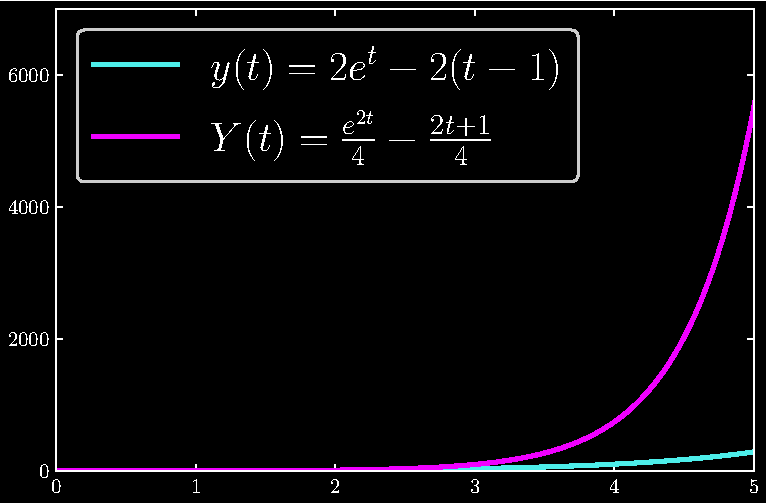
\includegraphics[width=1.0\textwidth]{chap1/sec1.6/chap1sec1.6ex9.eps}
\end{center}

% QUESTION 10
\qs{1.6.10}{Compare the linear equation \(y' = y\) to the separable equation \(y' = y^{2}\) starting from \(y \!\left( 0 \right) = 1\). Which solution \(y \!\left( t \right) \) must grow faster? It grows so fast that it blows up to \(y \!\left( T \right) = \infty\) at what time \(T\)?}

Solving the equations gives us:

\(\bm{y' = y: }\)
\begin{alignat*}{3}
	&\implies && \frac{d y}{d t} && = y \\
	&\implies && \int^{y \!\left( t \right) }_{y \!\left( 0 \right) } \frac{du}{u}  && = \int^{t}_{0}  \, dt  \\
	&\implies && \ln\left( y \!\left( t \right)  \right) - \ln\left( y \!\left( 0 \right)  \right) && = t \\
	&\implies && y \!\left( t \right) && = e^{t}
\end{alignat*}

\(\bm{y' = y^{2}:}\)
\begin{alignat*}{3}
	&\implies && \frac{d y}{d t} && = y^{2} \\
	&\implies && \int^{y \!\left( t \right) }_{y \!\left( 0 \right) } \frac{du}{u^{2}} && = \int^{t}_{0}  \, dt   \\
	&\implies && \frac{1}{y \!\left( 0 \right) } - \frac{1}{y \!\left( t \right) } && = t \\
	&\implies && y \!\left( t \right) && = \frac{1}{1 - t}
\end{alignat*}

Intuitively, we must have the solution \(y \!\left( t \right) \) to \(y' = y^{2}\) grow faster, assuming that \(y^{2} > y\). But as time approaches \(t = 1\), we see that the solution to \(y' = y^{2}\) hits an asymptotic point, namely
\[
	\lim\limits_{t \to 1} y \!\left( t \right) = \lim\limits_{t \to 1} \frac{1}{1 - t} = \infty
\]

% QUESTION 11
\qs{1.6.11}{\(Y' = 2Y\) has a larger growth factor (because \(a = 2\)) than \(y' = y + q \!\left( t \right) \). What source \(q \!\left( t \right) \) would be needed to keep \(y \!\left( t \right) = Y \!\left( t \right) \) for all time?}

Assume that \(Y \!\left( 0 \right) = y \!\left( 0 \right) \). Solving both equations, we find

\(\bm{Y' = 2Y:}\) Using integrating factor \(e^{-2t}\):
\begin{alignat*}{3}
	&\implies && Y' - 2Y && = 0 \\
	&\implies && \!\left( e^{-2t}Y \right)' && = 0 \\
	&\implies && e^{-2t} Y \!\left( t \right) - Y \!\left( 0 \right) && = 0 \\
	&\implies && Y \!\left( t \right) && = Y \!\left( 0 \right) e^{2t}
\end{alignat*}

\(\bm{y' = y + q \!\left( t \right) :}\) Using integrating factor \(e^{-t}\):
\begin{alignat*}{3}
	&\implies && y' - y && = q \!\left( t \right)  \\
	&\implies && \!\left( e^{-t}y \right)' && = e^{-t}q \!\left( t \right)  \\ 
	&\implies && e^{-t} y \!\left( t \right) - y \!\left( 0 \right) && = \int^{t}_{0} e^{-s}q \!\left( s \right)  \, ds \\
	&\implies && y \!\left( t \right) && = y \!\left( 0 \right) e^{t} + e^{t} \int^{t}_{0} e^{-s}q \!\left( s \right)  \, ds 
\end{alignat*}

For \(y \!\left( t \right) = Y \!\left( t \right) \) for all time \(t\), we need to have
\begin{alignat*}{3}
	&\implies && y \!\left( 0 \right) e^{t} + e^{t} \int^{t}_{0} e^{-s} q \!\left( s \right)  \, ds && = Y \!\left( 0 \right) e^{2t}  \\
	&\implies && \int^{t}_{0} e^{-s} q \!\left( s \right)  \, ds   && = Y \!\left( 0 \right) e^{t} - Y \!\left( 0 \right) \\
	& && && = Y \!\left( 0 \right) \!\left( e^{t} - 1 \right) 
\end{alignat*}
Immediately, we can see that if
\[
	q \!\left( t \right) = Y \!\left( 0 \right) e^{2t}
\]
Then we have the desired equality. We could have also derived this solution by taking our \(Y \!\left( t \right) \) and substituting it into the second equation:
\begin{alignat*}{3}
	&\implies && 2Y \!\left( 0 \right) e^{2t} - Y \!\left( 0 \right) e^{2t} && = q \!\left( t \right)  \\
	&\implies && Y \!\left( 0 \right) e^{2t} && = q \!\left( t \right)  \\ 
\end{alignat*}

% QUESTION 12
\qs{1.6.12}{Starting from \(y \!\left( 0 \right) = Y \!\left( 0 \right) = 1\), does \(y \!\left( t \right) \) or \(Y \!\left( t \right) \) eventually become larger?
\[
	\frac{d y}{d t} = 2y + e^{t} \qquad \frac{d Y}{d t} = Y + e^{2t}.
\]}

\(\bm{\frac{d y}{d t}  = 2y + e^{t}:}\) Using integrating factor \(e^{-2t}\), derive:
\begin{alignat*}{3}
	&\implies && \frac{d y}{d t} - 2y && = e^{t} \\
	&\implies && \!\left( e^{-2t}y \right)' && = e^{-t}  \\
	&\implies && e^{-2t} y \!\left( t \right) - y \!\left( 0 \right) && = \int^{t}_{0} e^{-s} \, ds \\
	&\implies && y \!\left( t \right) && = y \!\left( 0 \right) e^{2t} + e^{2t} \!\left( 1 - e^{-t} \right) \\
	& && && = 2e^{2t} - e^{t}
\end{alignat*}

\(\bm{\frac{d Y}{d t}  = Y + e^{2t}}:\) Using integrating factor \(e^{-t}\), derive:
\begin{alignat*}{3}
	&\implies && \frac{d Y}{d t} - Y && = e^{2t}  \\
	&\implies && \!\left( e^{-t}Y \right)' && = e^{t} \\ 
	&\implies && e^{-t} Y \!\left( t \right) - Y \!\left( 0 \right) && = \int^{t}_{0} e^{s} \, ds \\
	&\implies && Y \!\left( t \right) && = Y \!\left( 0 \right) e^{t} + e^{t} \!\left( e^{t} - 1 \right) \\
	& && && = e^{2t}
\end{alignat*}

Concluding, we see that \(y \!\left( t \right) > Y \!\left( t \right) \) for all time \(t\). We know this since \(e^{2t} > e^{t}\) for all time \(t\), so the subtraction of the \(e^{t}\) term in \(y \!\left( t \right) \) never outpaces the addition of the \(2\) factor on the \(e^{2t}\) term.

\vspace{12pt}

% QUESTION 13
\qs{1.6.13}{What is the factor \(G \!\left( s,s \right) \) in zero time? Find \(G \!\left( s, \infty \right) \) if \(a = -1\) and if \(a = 1\).}

Over zero time, we must have
\[
	G \!\left( s,s \right) = e^{\int^{s}_{s} a \!\left( T \right)  \, dT } = e^{0} = 1
\]
If \(a = -1\), then
\[
	G \!\left( s, \infty \right) = e^{-\int^{\infty}_{s}  \, dT } = 0
\]
And if \(a = 1\), then
\[
	G \!\left( s, \infty \right) = e^{\int^{\infty}_{s}  \, dT } = \infty
\]

% QUESTION 14
\qs{1.6.14}{Explain the important statement after equation (13): \textit{The growth factor \(G \!\left( s, t \right) \) is the solution to \(y' = a \!\left( t \right) y + \delta \!\left( t - s \right) \)}. The source \(\delta \!\left( t - s \right) \) deposits \(\$1\) at time \(s\).}

We solve this equation with integrating factor \(e^{-\int^{t}_{0} a \!\left( T \right)  \, dT }\):
\begin{alignat*}{3}
	&\implies && y' - a \!\left( t \right) y && = \delta \!\left( t - s \right)  \\
	&\implies && \!\left( e^{-\int^{t}_{0} a \!\left( T \right)  \, dT } y \right)' && = e^{-\int^{t}_{0} a \!\left( T \right)  \, dT } \delta \!\left( t - s \right)  \\
	&\implies && e^{-\int^{t}_{0} a \!\left( T \right)  \, dT } y \!\left( t \right) - y \!\left( 0 \right) && = \int^{t}_{0} e^{-\int^{t}_{0} a \!\left( T \right)  \, dT } \delta \!\left( t - s \right)  \, dt \\
	& && && = e^{-\int^{s}_{0} a \!\left( T \right)  \, dT } \\
	&\implies && y \!\left( t \right) && = \!\left( e^{\int^{t}_{0} a \!\left( T \right)  \, dT } \right) \!\left( e^{-\int^{s}_{0} a \!\left( T \right)  \, dT } \right) \\
	& && && = e^{\int^{t}_{s} a \!\left( T \right)  \, dT } \\
	& && && = G \!\left( s,t \right) 
\end{alignat*}

% QUESTION 15
\qs{1.6.15}{Now explain this meaning of \(G \!\left( s,t \right) \) when \(t\) \textit{is less than} \(s\). We go backwards in time. \textit{For} \(t < s\), \(G \!\left( s,t \right) \) \textit{is the value at time }\(t\) \textit{that will grow to equal} \(1\) \textit{at time} \(s\).

\vspace{12pt}

When \(t = 0\), \(G \!\left( s, 0 \right) \) is the ``present value" of a promise to pay \(\$1\) at time \(s\). If the interest rate is \(a = 0.1 = 10\%\) per year, what is the present value \(G \!\left( s,0 \right) \) of a million dollar inheritance promised in \(s = 10\) years?}

When \(t < s\), we necessarily have
\[
	G \!\left( s,t \right) = e^{\int^{t}_{s} a \!\left( T \right)   \, dT } = e^{-\int^{s}_{t} a \!\left( T \right)  \, dT } = \frac{1}{e^{\int^{s}_{t} a \!\left( T \right)  \, dT }}
\]

As \(t \rightarrow s\), \(G \!\left( s, t \right) \rightarrow 1\), and particularly -- the growth factor grows \textit{to} 1 from below. Once \(t = s \), \(G \!\left( s, t \right) = 1\). Intuitively, \(G \!\left( s,t \right) \) simply gives us the portion of the deposit at time \(t < s\); once the time hits \(s\), the deposit has fully grown to the desired amount. 

For the second question, we have
\[
	G \!\left( s,0 \right) = e^{\int^{0}_{s} 0.1 \, dT } = e^{-0.1s}
\]
For \(s = 10\) years, the present value of the million dollar inheritance is
\[
	G \!\left( 10, 0 \right) = \frac{1}{e} \quad \implies \quad 10^{6} G \!\left( 10,0 \right) 
\]

% QUESTION 16
\qs{1.6.16}{\begin{enumerate}[label=(\alph*)]
	\item What is the growth factor \(G \!\left( s,t \right) \) for the equation \(y' = \!\left( \sin t \right) y + Q \sin t\)?
	\item What is the null solution \(y_{n} = G \!\left( 0,t \right) \) to \(y' = \!\left( \sin t \right) y\) when \(y \!\left( 0 \right) = 1\)?
	\item What is the particular solution \(y_{p} = \int^{t}_{0} G \!\left( s,t \right) Q \sin s \, ds  \) ?
\end{enumerate}}

(a) The growth factor is given by
\[
	G \!\left( s,t \right) = \exp\left( \int^{t}_{s} \sin T \, dT  \right) = \exp\left( \cos s - \cos t \right)
\]

(b) The null solution is given by
\begin{alignat*}{3}
	&\implies && y' - \!\left( \sin t \right) y && = 0 \\
	&\implies && \!\left( e^{-\int^{t}_{0} \sin T \, dT } y \right)' && = 0  \\
	&\implies && e^{-\int^{t}_{0} \sin T \, dT } y \!\left( t \right) - y \!\left( 0 \right) && = 0 \\
	&\implies && y_{n} \!\left( t \right) && = e^{\int^{t}_{0} \sin T \, dT } \\
	& && && = e^{1 - \cos t}
\end{alignat*}

Which is equal to
\[
	G \!\left( 0, t \right) = e^{1 - \cos t}
\]

(c) The particular solution is given by the bracketed term:
\begin{alignat*}{3}
	&\implies && y' - \!\left( \sin t \right) y && = Q \sin t \\
	&\implies && \!\left( e^{-\int^{t}_{0} \sin T \, dT }y \right)' && = e^{-\int^{t}_{0} \sin T \, dT } Q \sin t \\ 
	&\implies && e^{-\int^{t}_{0} \sin T \, dT } y \!\left( t \right) - y \!\left( 0 \right) && = \int^{t}_{0} e^{-\int^{s}_{0} \sin T \, dT } Q \sin s \, ds \\ 
	&\implies && y \!\left( t \right) && = e^{1 - \cos t} + \int^{t}_{0} e^{\int^{t}_{s} \sin T \, dT } Q \sin s \, ds \\
	& &&  && = e^{1 - \cos t} + \int^{t}_{0} e^{\cos s - \cos t} Q \sin s \, ds  \\
	& && && = e^{1 - \cos t} + e^{-\cos t} \int^{t}_{0} e^{\cos s} Q \sin s \, ds \\
	& && && = e^{1 - \cos t} + Qe^{-\cos t} \!\left( e - e^{\cos t} \right) \\
	& && && = \underbrace{e^{1 - \cos t}}_{y_{n}} + \underbrace{Q \!\left( e^{1 - \cos t} - 1 \right) }_{y_{p}}
\end{alignat*}

As expected, \(y \!\left( 0 \right) \) gives us \(1\).

\vspace{12pt}

% QUESTION 17
\qs{1.6.17}{\begin{enumerate}[label=(\alph*)]
	\item What is the growth factor \(G \!\left( s,t \right) \) for the equation \(y' = y / \!\left( t + 1 \right) + 10\)? 
	\item What is the null solution \(y_{n} = G \!\left( 0,t \right) \) to \(y' = y / \!\left( t + 1 \right) \) with \(y \!\left( 0 \right) = 1\)?
	\item What is the particular solution \(y_{p} = 10 \int^{t}_{0} G \!\left( s,t \right)  \, ds  \)?
\end{enumerate}}

(a) The growth factor \(G \!\left( s,t \right) \) is given by
\begin{align*}
	G \!\left( s,t \right) &= \exp\left( \int^{t}_{s} \frac{1}{T + 1} \, dT \right) \\
			       & = \exp\left( \ln\left( t + 1 \right) - \ln\left( s + 1 \right) \right) \\
			       & = \exp\left( \ln\left( \frac{t + 1}{s + 1} \right) \right) \\
			       & = \frac{t + 1}{s + 1}
\end{align*}

(b) We derive the null solution as
\begin{alignat*}{3}
	&\implies && y' - \frac{y}{t + 1} && = 0 \\
	&\implies && \!\left( e^{-\int^{t}_{0} 1 / \!\left( T + 1 \right)  \, dT } y \right)' && = 0  \\ 
	&\implies && e^{-\int^{t}_{0} 1 / \!\left( T + 1 \right)  \, dT } y \!\left( t \right) - y \!\left( 0 \right) && = 0 \\
	&\implies && y_{n} \!\left( t \right) && = e^{\int^{t}_{0} 1 / \!\left( T + 1 \right)  \, dT } \\
	& && && = t + 1 
\end{alignat*}

Which is equal to
\[
	G \!\left( 0, t \right) = t + 1
\]

(c) The particular solution is given in brackets
\begin{alignat*}{3}
	&\implies && y' - \frac{y}{t + 1} && = 10 \\
	&\implies && \!\left( e^{-\int^{t}_{0} 1 / \!\left( T + 1 \right)  \, dT } y \right)' && = 10 e^{-\int^{t}_{0} 1 / \!\left( T + 1 \right)  \, dT } \\ 
	&\implies && e^{-\int^{t}_{0} 1 / \!\left( T + 1 \right)  \, dT } y \!\left( t \right) - y \!\left( 0 \right) && = \int^{t}_{0} \frac{10}{s + 1} \, ds \\
	&\implies && y \!\left( t \right) && = \underbrace{t + 1}_{y_{n}} + \underbrace{10 \!\left( t + 1 \right) \ln\left( t + 1 \right)}_{y_{p}}
\end{alignat*}

\vspace{12pt}

As expected, \(y \!\left( 0 \right) \) yields \(1\).

\vspace{12pt}

% QUESTION 18
\qs{1.6.18}{Why is \(G \!\left( t, s \right) = 1 / G \!\left( s, t \right) \)? Why is \(G \!\left( s, t \right) = G \!\left( s, S \right) G \!\left( S, t \right) \)?}

By definition,
\[
	G \!\left( t,s \right) = \exp\left( \int^{s}_{t} a \!\left( T \right)  \, dT  \right)
\]
By the Fundamental Theorem of Calculus, flipping the bounds of integration changes the sign of the integral:
\begin{align*}
	G \!\left( t,s \right) & = \exp\left( \int^{s}_{t} a \!\left( T \right)  \, dT  \right) \\
		 & = \exp\left( -\int^{t}_{s} a \!\left( T \right)  \, dT  \right) \\
		 & = 1 / \exp\left( \int^{t}_{s} a \!\left( T \right)  \, dT  \right) \\
		 & = 1 / G \!\left( s, t \right)  
\end{align*}

Secondly, suppose that \(s \le S \le t\). Then
\begin{align*}
	G \!\left( s, t \right)  & = \exp\left( \int^{t}_{s} a \!\left( T \right) \, dT  \right) \\
	 & = \exp\left( \int^{S}_{s} a \!\left( T \right)  \, dT + \int^{t}_{S} a \!\left( T \right)  \, dT  \right)  \\
	 & = \exp\left( \int^{S}_{s} a \!\left( T \right)  \, dT  \right) \exp\left( \int^{t}_{S} a \!\left( T \right)  \, dT  \right) \\
	 & = G \!\left( s, S \right) G \!\left( S, t \right) 
\end{align*}

% QUESTION 19	
\qs{1.6.19}{(recommended) If \(dy / dt = ay + qe^{i \omega t}\), with \(t\) in seconds and \(y\) in meters, what are the units for \(a\) and \(q \) and \(\omega \)?}

The units for \(a\), \(q \), and \(\omega \) are in \(1 / \text{s}\), \(m/s\), and \(1/s\), respectively. We have \(a\) and \(q \) as frequencies, and \(q \) is velocity.

\vspace{12pt}

% QUESTION 20
\qs{1.6.20}{The logistic equation \(dy / dt = ay - by^{2}\) often measures the time \(t\) in years (and \(y\) counts people). What are the units of \(a\) and \(b\)?}

The units for \(a\) and \(b\) are \(1 / \text{year}\) and \(1 / \!\left( \text{people} \cdot \text{year} \right) \), respectively.

\vspace{12pt}

% QUESTION 21
\qs{1.6.21}{Newton's Law is \(m \frac{d^{2} y}{d t^{2}} + ky = F \). If the mass \(m\) is in grams, \(y\) is in meters, and \(t\) is in seconds, what are the units of the stiffness \(k\) and the force \(F\)?}

The units for \(k\) and \(F\) are \(g / s^{2}\) and \(g \cdot m / s^{2}\), respectively.

\vspace{12pt}

% QUESTION 22
\qs{1.6.22}{Why is our favorite example \(y' = y + 1\) very unsatisfactory dimensionally? Solve it anyway starting from \(y \!\left( 0 \right) = -1\) and from \(y \!\left( 0 \right) = 0\).}

We have \(y'\) represented in units of something per unit time, while \(y\) is in units of something, and ambiguity as to the unit of the constant \(1\). Nevertheless, we solve it using the integrating factor \(e^{-t}\):
\begin{alignat*}{3}
	&\implies && y' - y && = 1 \\
	&\implies && \!\left( e^{-t}y \right)' && = e^{-t} \\ 
	&\implies && e^{-t} y \!\left( t \right) - y \!\left( 0 \right) && = \int^{t}_{0} e^{-s} \, ds \\
	&\implies && y \!\left( t \right) && = -e^{t} + e^{t} \!\left(-e^{-t} + 1  \right) \\
	& && && = -1
\end{alignat*}

% QUESTION 23
\qs{1.6.23}{The difference equation \(Y_{n+1} = cY_{n} + Q_{n}\) produces \(Y_{1} = cY_{0} + Q_{0}\). Show that the next step produces \(Y_{2} = c^{2} Y_{0} + cQ_{0} + Q_{1}\). After \(N\) steps, the solution formula for \(Y_{N}\) is like the solution formula for \(y' = ay + q \!\left( t \right) \). Exponentials of \(a\) change to powers of \(c\), the null solution \(e^{at} y \!\left( 0 \right) \) becomes \(c^{N} Y_{0}\). The particular solution
\[
	Y_{N} = c^{N - 1} Q_{0} + \cdots + Q_{N - 1} \quad \text{is like} \quad y \!\left( t \right) = \int^{t}_{0} e^{a \!\left( t-s \right) q \!\left( s \right) } \, ds. 
\]}

By definition, we have
\begin{align*}
	Y_{2} & = cY_{1} + Q_{1} \\
	     & = c \!\left( c Y_{0} + Q_{0} \right) + Q_{1} \\ 
	     & = c^{2} Y_{0} + cQ_{0} + Q_{1}
\end{align*}

Moving onto \(Y_{3}\), we can derive
\begin{align*}
	Y_{3} & = cY_{2} + Q_{2} \\
	 & = c \!\left( c^{2}Y_{0} + cQ_{0} + Q_{1} \right)  \\ 
	 & = c^{3}Y_{0} + c^{2}Q_{0} + cQ_{1} + Q_{2}
\end{align*}

By now, a pattern emerges, from which we can conjecture that \(Y_{N}\) is of form
\[
	Y_{N} = \underbrace{c^{N} Y_{0}}_{y_{n}} + \underbrace{\sum_{i=0}^{N-1} c^{N - 1 - i}Q_{i}}_{y_{p}}
\]

% QUESTION 24
\qs{1.6.24}{Suppose a fungus doubles in size every day, and it weighs a pound after 10 days. If another fungus was twice as large at the start, would it weigh a pound in 5 days?}

By premise, we must have
\[
	y \!\left( t \right) = C2^{t}
\]
where \(t\) is in units of days. Since \(y \!\left( 10 \right) = 1\), the constant \(C\) must equal
\[
	C = \frac{1}{2^{10}}
\]
So at \(t = 0\), the fungus must be \(1 / 2^{10}\) pounds. Suppose now the second fungus starts at size \(2 / 2^{10} = 1 / 2^{9}\). Then when \(t = 9\), we have
\[
	y \!\left( 9 \right) = \frac{1}{2^{9}} \cdot 2^{9} = 1
\]
Thus it would take 9 days for the second fungus that is twice as large as the first to grow to one pound.

\newpage
\subsection{\textsf{1.7 - The Logistic Equation}}
% QUESTION 1
\qs{1.7.1}{If \(y \!\left( 0 \right) = a/2b\), the halfway point on the \(S\)-curve is at \(t = 0\). Show that \(d = b\) and \(y \!\left( t \right) = \displaystyle{\frac{a}{de^{-at} + b} = \frac{a}{b} \frac{1}{e^{-at} + 1}}\). Sketch the curve from \(y_{-\infty} = 0\) to \(y_{\infty} = \displaystyle{\frac{a}{b}}\).}

Given the logistic equation
\[
	\frac{d y}{d t} = ay - by^{2}
\]
We let \(z = 1/y\), implying that
\[
	\frac{d z}{d t} = -\frac{1}{y^{2}} \frac{d y}{d t} 
\]
Thus we can rewrite the logistic equation as
\[
	\frac{d z}{d t} = -\frac{1}{y^{2}} \!\left( ay - by^{2} \right) = - \!\left( \frac{a}{y} - b \right) = -az + b
\]
which has solution
\begin{alignat*}{3}
	&\implies && \frac{d z}{d t}  + az && = b \\
	&\implies && \!\left( e^{at}z \right)' && = b e^{at} \\ 
	&\implies && e^{at} z \!\left( t \right) - z \!\left( 0 \right) && = \int^{t}_{0} be^{at} \, dt \\
	& && && = \frac{b}{a} \!\left( e^{at} - 1 \right)  \\
	&\implies && z \!\left( t \right) && = e^{-at} z \!\left( 0 \right) + \frac{b}{a} \!\left( 1 - e^{-at} \right) 
\end{alignat*}

Now let \(d/a = z \!\left( 0 \right) - b/a\). Since \(z \!\left( 0 \right) = 1/y \!\left( 0 \right) \), we have \(d = a / y \!\left( 0 \right) - b\). Then we may write
\[
	z \!\left( t \right) = \frac{d e^{-at} + b}{a}
\]
Finally implying
\[
	y \!\left( t \right) = \frac{a}{de^{-at} + b}
\]
Now, for \(\displaystyle{y \!\left( 0 \right) = \frac{a}{2b}}\), our parameter \(d\) is
\[
	d = \frac{a}{a / 2b} - b = 2b - b = b
\]
enabling us to conclude
\[
	y \!\left( t \right) = \frac{a}{b} \frac{1}{e^{-at} + 1}
\]
The curve is graphed as

\begin{center}
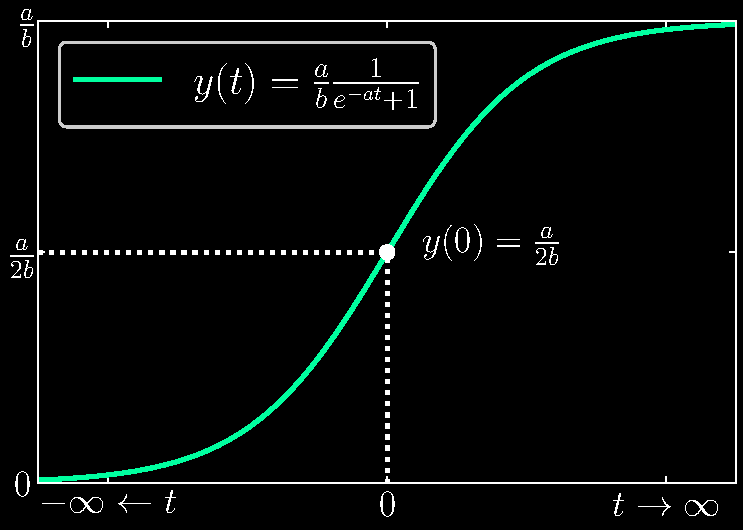
\includegraphics[width=1.0\textwidth]{chap1/sec1.7/chap1sec1.7ex1.eps}
\end{center}

% QUESTION 2
\qs{1.7.2}{If the carrying capacity of the Earth is \(K = a/b = 14\) billion people, what will be the population at the inflection point? What is \(dy/dt\) at that point? The actual population was 7.14 billion on January 1, 2014.}

The inflection point is at \(y \!\left( t \right) = a / 2b\), or
\[
	y \!\left( t \right) = \frac{a}{2b} = 7 \text{ billion people}
\]
The natural growth rate \(a\) is estimated to be \(.029\) per year. Then we have
\[
	b = \frac{a}{K} = \frac{.029}{14 \cdot 10^{9}} \approx 2.1 \cdot 10^{-12}
\]
which corresponds to \(dy/dt\):
\[
	\frac{d y}{d t} = 0.029 \!\left( 7 \cdot 10^{9} \right)  - \!\left( 2.1 \cdot 10^{-12} \right) \!\left( 7 \cdot 10^{9} \right)^{2} \approx 10^{8} 
\]

% QUESTION 3
\qs{1.7.3}{Equation (18) must give the same formula for the solution \(y \!\left( t \right) \) as equation (16). If the right side of (18) is called \(R\), we can solve that equation for \(y\):
\[
	y = R \!\left( 1 - \frac{b}{a}y \right) \quad \rightarrow \quad \!\left( 1 + R \frac{b}{a} \right) y = R \quad \rightarrow \quad y = \frac{R}{\!\left( 1 + R \frac{b}{a} \right) }
\]
Simplify that answer by algebra to recover equation (16) for \(y \!\left( t \right) \).}

Equation (18) is given by
\[
	\frac{y}{1 - \frac{b}{a}y} = e^{at} \frac{y \!\left( 0 \right) }{1 - \frac{b}{a} y \!\left( 0 \right) } = R
\]

Which we solve by
\begin{alignat*}{2}
	\implies && y & = R \!\left( 1 - \frac{b}{a}y \right)  \\
	\implies && \!\left( 1 + R \frac{b}{a} \right) y & = R \\ 
	\implies && y & = \frac{R}{\!\left( 1 + R \frac{b}{a} \right) } 
\end{alignat*}

Now, define \(d\) as
\[
	d = \frac{a}{y \!\left( 0 \right) - b}
\]
Then we may write \(R\) as
\[
	R = e^{at} \!\left( \frac{a}{d} \right) 
\]
which is more compact to work with. Then we continue with
\begin{alignat*}{3}
	\implies && y & = \frac{e^{at} \!\left( \frac{a}{d} \right) }{1 + \!\left( \frac{b}{a} \right) e^{at} \!\left( \frac{a}{d} \right) } \\
	\implies && y & = \frac{e^{at} \!\left( \frac{a}{d} \right) }{\!\left( d + be^{at} \right) / d}  \\ 
	\implies && y & = \frac{ae^{at}}{d + be^{at}} \\
	\implies && y & = \frac{a}{de^{-at} + b}
\end{alignat*}

Deriving the desired result, equation (16).

\vspace{12pt}

% QUESTION 4
\qs{1.7.4}{Change the logistic equation to \(y' = y + y^{2}\). Now the nonlinear term is positive, and \textit{cooperation of} \(y\) \textit{with} \(y\) promotes growth. Use \(z = 1/y\) to find and solve a linear equation for \(z\), starting from \(z \!\left( 0 \right) = y \!\left( 0 \right) = 1\). Show that \(y \!\left( T \right) = \infty\) when \(e^{-T} = 1/2\). Cooperation looks bad, the population will explode at \(t = T\).}

Given \(y' = y + y^{2}\), let \(z = 1/y\). Then
\begin{alignat*}{3}
	\implies && z' & = -\frac{1}{y^{2}}y' \\
	&& & = -\frac{1}{y} - 1 \\ 
	&& & = - \!\left( z + 1 \right) 
\end{alignat*}

Writing \(z'\) as \(\displaystyle{\frac{d z}{d t} }\) and separating variables, we can write

\begin{alignat*}{2}
	\implies && \frac{d z}{d t}  & = - \!\left( z + 1 \right)  \\
	\implies && - \int^{z \!\left( t \right) }_{z \!\left( 0 \right) } \frac{dz}{z + 1}  & = \int^{t}_{0} \, dt  \\ 
	\implies && -\ln\left( z \!\left( t \right) + 1 \right) + \ln\left( 2 \right) & = t \\
	\implies && \ln\left( \frac{2}{z \!\left( t \right)  + 1} \right) & = t \\
	\implies && \frac{2}{z \!\left( t \right) + 1} & = e^{t} \\
	\implies && z \!\left( t \right) & = 2e^{-t} - 1 \\
	\implies && y \!\left( t \right) & = \frac{1}{2e^{-t} - 1}
\end{alignat*}

Clearly, we have \(z \!\left( 0 \right) = y \!\left( 0 \right) = 1\). Now, suppose that we have
\[
	\lim\limits_{T \to \ln\left( 2 \right)} e^{-T} = \frac{1}{2}
\]
Then it must follow that
\[
	\lim\limits_{T \to \ln\left( 2 \right)}  y \!\left( t \right) = \lim\limits_{T \to \ln\left( 2 \right)} \frac{1}{2e^{-t} - 1} = \infty
\]
Which indicates an explosion of population as \(T\) approaches \(\ln\left( 2 \right)\).

\vspace{12pt}

% QUESTION 5
\qs{1.7.5}{The US population grew from 313,873,685 in 2012 to 316,128,839 in 2014. If it were following a logistic \(S\)-curve, what equations would give you \(a\), \(b\), \(d\) in the formula (4)? Is the logistic equation reasonable and how to account for immigration?}

Suppose we set \(t = 0\) as corresponding to 2012. Then \(t = 2\) corresponds to 2014. We have
\[
	y \!\left( 0 \right) = \frac{a}{d + b} = 313,873,685 \quad \text{and} \quad y \!\left( 2 \right) = \frac{a}{de^{-2a} + b} = 316,128,839
\]
Due to the nonlinearity, it is not readily clear how we identify the corresponding logistic equation that fits these points. As far as immigration goes, suppose we add the constant harvesting rate \(-h\) to the logistic equation:
\[
	\frac{d y}{d t} = ay - by^{2} - h
\]
Since immigration would lead to an \textit{increase} in \(dy/dt\), we must have \(h < 0\). By contrast, \textit{emigration decreases} \(dy/dt\), corresponding to \(h > 0\).

\vspace{12pt}

% QUESTION 6
\qs{1.7.6}{The \textbf{Bernoulli equation} \(y' = ay - by^{n}\) has competition term \(by^{n}\). Introduce \(z = y^{1-n}\) which matches the logistic case when \(n = 2\). Follow equation (4) to show that \(z' = \!\left( n - 1 \right) \!\left( -az + b \right) \). Write \(z \!\left( t \right) \) as in (5)-(6). Then you have \(y \!\left( t \right) \).}

Let \(z = y^{1-n}\). Then we have
\[
	z' = \!\left( 1-n \right) y^{-n} y'
\]

and are able to derive
\begin{alignat*}{2}
	\implies && z' & = \!\left( 1 - n \right) \!\left(ay^{1-n} - b\right) \\
	&& & = \!\left( n - 1 \right) \!\left( -az + b \right)
\end{alignat*}
Separating variables, we can conclude with
\begin{alignat*}{2}
	\implies && \frac{d z}{d t}  & = \!\left( n - 1 \right) \!\left( -az + b \right)  \\
	\implies && \int^{z \!\left( t \right) }_{z \!\left( 0 \right) } \frac{dz}{-az + b}  & = \int^{t}_{0} \!\left( n - 1 \right)  \, dt  \\ 
	\implies && -\frac{1}{a} \!\left( \ln\left( -az \!\left( t \right) + b \right) - \ln\left( -a z \!\left( 0 \right) + b \right) \right) & = \!\left( n - 1 \right) t \\
	\implies && \frac{-a z \!\left( t \right) + b}{-a z \!\left( 0 \right) + b} & = e^{-a \!\left( n - 1 \right) t} \\
	\implies && z \!\left( t \right) & = -\frac{1}{a} \!\left( \!\left( -a z \!\left( 0 \right) + b \right) e^{a \!\left( 1 - n \right) t} - b \right) \\ 
		 && & = z \!\left( 0 \right) e^{a \!\left( 1 - n \right) t} - \frac{b}{a} \!\left( e^{a \!\left( 1 - n \right) t} - 1 \right) 
\end{alignat*}

Now, define \(d\) as
\[
	d = \frac{a}{y \!\left( 0 \right) } - b
\]
Then we have
\[
	z \!\left( t \right) = \frac{de^{a \!\left( 1 - n \right) t} + b}{a}
\]
Finally implying
\[
	y \!\left( t \right) = \frac{a}{de^{-a \!\left( n - 1 \right) t} + b}
\]

% QUESTION 7
\qs{1.7.7}{\(y' = y - y^{2}\) is solved by \(y \!\left( t \right) = 1 / \!\left( de^{-t} + 1 \right) \). This is an \(S\)-curve when \(y \!\left( 0 \right) = 1/2\) and \(d = 1\). But show that \(y \!\left( t \right) \) is very different if \(y \!\left( 0 \right) > 1\) or if \(y \!\left( 0 \right) < 0\).

If \(y \!\left( 0 \right) = 2\) then \(d = \frac{1}{2} - 1 = -\frac{1}{2}\). Show that \(y \!\left( t \right) \rightarrow 1\) from above.

If \(y \!\left( 0 \right) = -1\) then \(d = \frac{1}{-1} - 1 = -2\). At what time \(T\) is \(y \!\left( T \right) = -\infty\)?}

Suppose that \(y \!\left( 0 \right) > 1\). Then we have
\[
	d = \frac{1}{y \!\left( 0 \right) } - 1 < 0
\]
We can also determine that \(y \!\left( 0 \right) < 0\) leads to the same result: \(d\) \textit{is negative.} When \(d\) is negative, then we have a discontinuity at \(t\) when \(de^{-t} + 1 = 0\). The \(S\)-curve has no such discontinuity, so there is a stark difference when the initial condition \(y \!\left( 0 \right) \) meets the aforementioned values.

Suppose that \(y \!\left( 0 \right) = 2\). Then \(d = -1/2\). The steady state is \(a/b = 1/1 = 1\). We have
\[
	\lim\limits_{t \to \infty} \frac{1}{-\frac{1}{2}e^{-t} + 1} = 1
\]

and \(y \!\left( t \right) \) approaches 1 from above.

\begin{center}
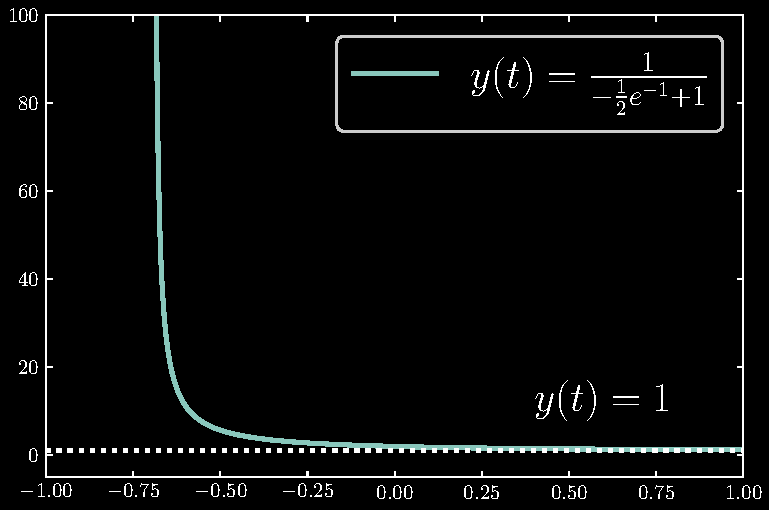
\includegraphics[width=1.0\textwidth]{chap1/sec1.7/chap1sec1.7ex7a.eps}
\end{center}

In the case where \(y \!\left( 0 \right) = -1\), then \(d = -2\). 
\[
	y \!\left( t \right) = \frac{1}{-2e^{-t} + 1}
\]
The point where approaching \(t = T\) corresponds to \(y \!\left( t \right) \) tending towards \(-\infty\) is where the denominator approaches zero. This time \(t = T\) is thus at
\begin{alignat*}{2}
	\implies && -2e^{-T} + 1 & = 0 \\
	\implies && e^{-T} & = \frac{1}{2} \\ 
	\implies && T & = -\ln\left( \frac{1}{2} \right) \\
		 && & = \ln\left( 2 \right)
\end{alignat*}

\begin{center}
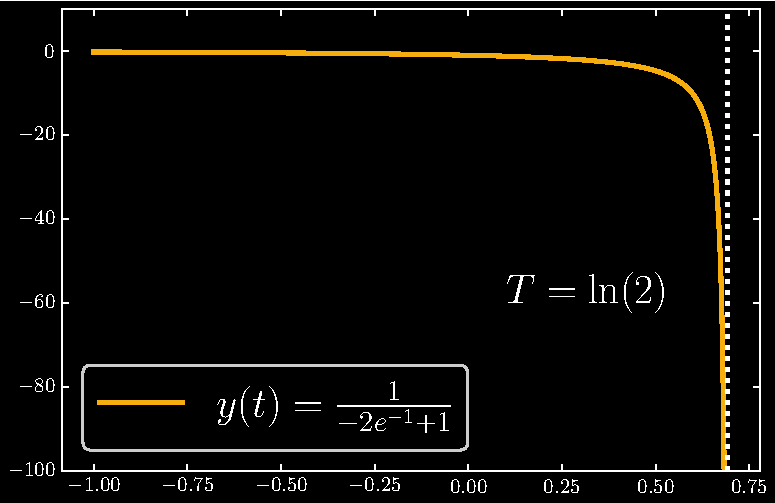
\includegraphics[width=1.0\textwidth]{chap1/sec1.7/chap1sec1.7ex7b.eps}
\end{center}

% QUESTION 8
\qs{1.7.8}{(recommended) Show those 3 solutions to \(y' = y - y^{2}\) in one graph! They start from \(y \!\left( 0 \right) = 1/2\) and 2 and \(-1\). The \(S\)-curve climbs from \(\frac{1}{2}\) to 1. Above that, \(y \!\left( t \right) \) descends from 2 to 1. Below the \(S\)-curve, \(y \!\left( t \right) \) drops from \(-1\) to \(-\infty\).

Can you see 3 regions in the picture? \textbf{Dropin curves above \(\bm{y = 1}\) and \(\bm{S}\)-curves sandwiched between 0 and 1 and dropoff curves below \(\bm{y = 0}\).}}

For the given initial conditions, we have solutions
\begin{align*}
	d_{1} & = \frac{1}{1/2} - 1 = 1 \\
	y_{1} \!\left( t \right)  & = \frac{1}{e^{-t} + 1} \\
	d_{2} & = \frac{1}{2} - 1 = -\frac{1}{2} \\
	y_{2} \!\left( t \right) & = \frac{1}{\!\left( -1/2 \right) e^{-t} + 1} \\
	d_{3} & = \frac{1}{-1} - 1 = -2 \\
	y_{3} & = \frac{1}{-2e^{-t} + 1}
\end{align*}

The functions we graph as
\begin{center}
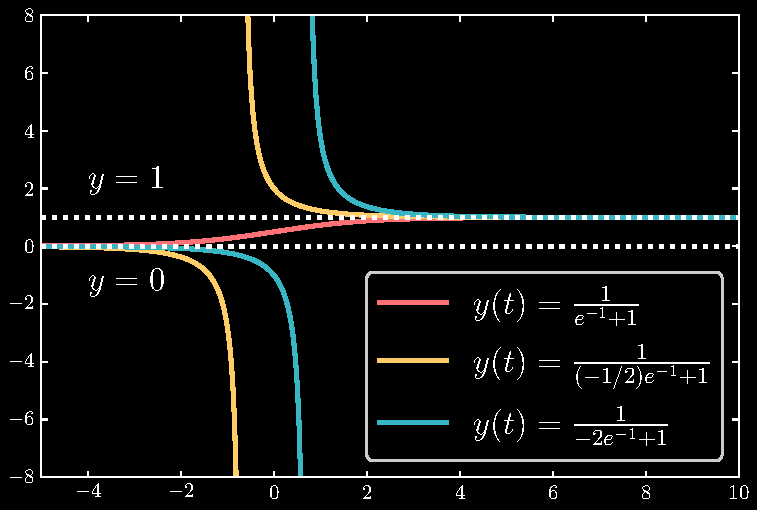
\includegraphics[width=1.0\textwidth]{chap1/sec1.7/chap1sec1.7ex8.eps}
\end{center}

The \(S\)-curve falls within the interval \(y \in \left( 0, \displaystyle{\frac{a}{b} = 1} \right) \), and when the initial conditions fall outside of that range, we end up with dropin and dropout curves that asymptotically approach the bounds of the interval.

\vspace{12pt}

% QUESTION 9
\qs{1.7.9}{Graph \(f \!\left( y \right) = y - y^{2}\) to see the unstable steady state \(Y  = 0\) and the stable \(Y = 1\). Then graph \(f \!\left( y \right) = y - y^{2} - 2/9\) with harvesting \(h = 2/9\). What are the steady states \(Y_{1}\) and \(Y_{2}\)? The 3 regions in Problem 8 now have \(Z\)-curves above \(y = 2/3\), \(S\)-curve sandwiched between \(1/3\) and \(2/3\), dropoff curves below \(y = 1/3\).}

For the harvesting equation, we have steady states
\[
	Y_{1}, Y_{2} = \frac{-1 \pm \sqrt{1 - 8/9}}{-2} = \frac{1}{3}, \frac{2}{3} 
\]
Allowing for the decomposition
\[
	f \!\left( y \right) = y - y^{2} - 2/9 = \!\left( Y_{1} - \frac{1}{3} \right) \!\left( Y_{2} - \frac{2}{3} \right) = 0
\]
At these steady states, we have
\[
	\frac{d f}{d y} = 1 - 2y; \frac{d f}{d y} \!\left(Y_{1} = \frac{1}{3} \right) = \frac{1}{3} \quad \text{and} \quad \frac{d f}{d y} \!\left(Y_{2} = \frac{2}{3} \right) = -\frac{1}{3}
\]
Concluding that \(Y_{1}\) is an \textbf{unstable} steady state and \(Y_{2}\) is a \textbf{stable} steady state. 

Graphically, we have

\begin{center}
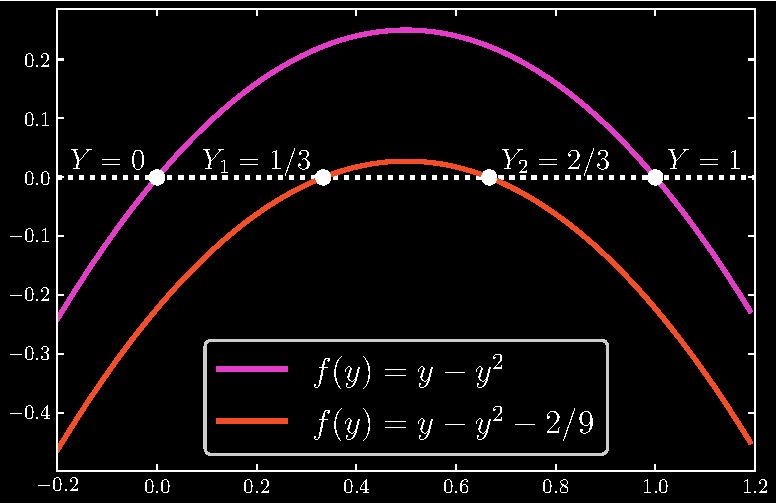
\includegraphics[width=1.0\textwidth]{chap1/sec1.7/chap1sec1.7ex9.eps}
\end{center}

% QUESTION 10
\qs{1.7.10}{What equation produces an \(S\)-curve climbing to \(y_{\infty} = K\) from \(y_{-\infty} = L\)?}

Our steady states are \(y_{\infty}, y_{-\infty} = K, L\). Then for the general equation \(f \!\left( y \right) = ay - by^{2} - h\), we must have
\begin{align*}
	aK - bK^{2} - h & = 0 \\
	aL - bL^{2} - h & = 0 
\end{align*}
Which simply screams matrix algebra to identify the unknown \(a\) and \(b\) parameters for a given harvesting term \(h\). We set up our matrix equation as such:
\[
	\underbrace{\begin{bmatrix}
		K & -K^{2} \\
		L & -L^{2} \\
\end{bmatrix}}_{A}
\begin{bmatrix}
	a \\
	b \\
\end{bmatrix}
=
\begin{bmatrix}
	h \\
	h \\
\end{bmatrix}
\]
Now, we have determinant
\[
	\det A = -KL^{2} + LK^{2} = LK \!\left( K - L \right) 
\]
which yields the inverse matrix
\[
	A^{-1} = \frac{1}{LK \!\left( K - L \right) }
	\begin{bmatrix}
		-L^{2} & K^{2} \\
		-L & K \\
	\end{bmatrix}
\]
Lastly, we find \(a\) and \(b\) to be
\[
	\begin{bmatrix}
		a \\
		b \\
	\end{bmatrix}
= \frac{1}{LK \!\left( K - L \right) }
\begin{bmatrix}
	-L^{2} & K^{2} \\
	-L & K \\
\end{bmatrix}
\begin{bmatrix}
	h \\
	h \\
\end{bmatrix}
\]
\begin{align*}
	a & = \frac{h}{LK \!\left( K - L \right) } \!\left( K^{2} - L^{2} \right)  \\
	 & = h \!\left( \frac{K + L}{KL} \right)  \\
	 & = \boxed{h \!\left( \frac{1}{K} + \frac{1}{L} \right)} \\
	b & = \frac{h}{LK \!\left( K - L \right) } \!\left( K - L \right) \\
	  & = \boxed{\frac{h}{KL}}
\end{align*}

% QUESTION 11
\qs{1.7.11}{\(y' = y - y^{2} - \frac{1}{4} = - \!\left( y - \frac{1}{2} \right)^{2}\) shows \textit{critical harvesting} with a double steady state at \(y = Y = \frac{1}{2}\). The layer of \(S\)-curves shrinks to that single line. Sketch a dropin curve that starts above \(y \!\left( 0 \right) = \frac{1}{2}\) and a dropoff curve that starts below \(y \!\left( 0 \right) = \frac{1}{2}\).}

Let's solve this equation. By separable variables, we find

\begin{alignat*}{3}
	\implies && \frac{d y}{d t}  & = y - y^{2} - \frac{1}{4} \\
	\implies && \int^{y \!\left( t \right) }_{y \!\left( 0 \right) } -\frac{dy}{\!\left( y - 1/2 \right)^{2}}  & = \int^{t}_{0}  \, dt  \\ 
	\implies && \frac{1}{y \!\left( t \right) - 1/2} - \frac{1}{y \!\left( 0 \right) - 1/2} & = t \\
	\implies && \frac{1}{y \!\left( t \right) - 1/2} & = t + \frac{1}{y \!\left( 0 \right) - 1/2} \\
	\implies && 1 & = \!\left( y \!\left( t \right) - 1/2 \right) \!\left( t + \frac{1}{y \!\left( 0 \right) - 1/2} \right) \\
	\implies && y \!\left( t \right) & = \frac{y \!\left( 0 \right) - 1/2}{y \!\left( 0 \right) t - t/2 + 1} + \frac{1}{2} \\
\end{alignat*}

From here, we may deduce that \(y \!\left( 0 \right) = 1/2\) implies
\[
	y \!\left( t \right) = \frac{1}{2}
\]
as expected. In other words, the ``\(S\)''-curve collapses into a horizontal line at the point of critical harvesting.

Suppose that we have cases in which \(y \!\left( 0 \right) = 1\) and \(y \!\left( 0 \right) = 0\). Then we can graph dropin and dropoff curves:

\begin{center}
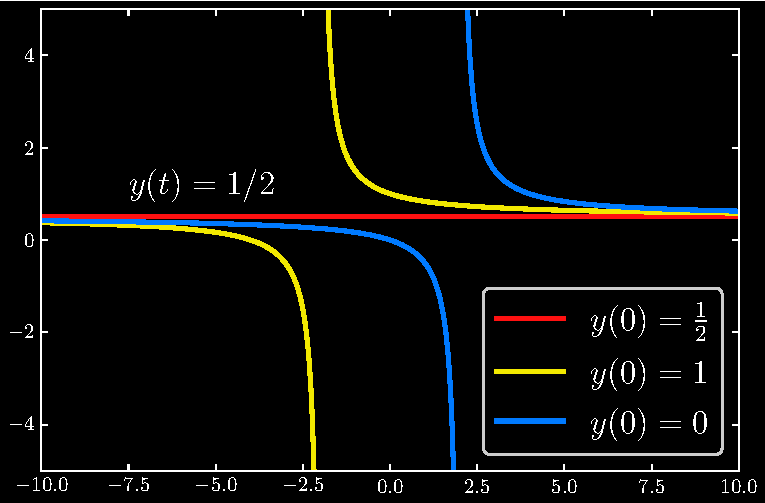
\includegraphics[width=1.0\textwidth]{chap1/sec1.7/chap1sec1.7ex11.eps}
\end{center}

% QUESTION 12
\qs{1.7.12}{Solve the equation \(y' = -\!\left( y - \frac{1}{2} \right)^{2}\) by substituting \(v = y - \frac{1}{2}\) and solving \(v' = -v^{2}\).}

See 1.7.11.

\vspace{12pt}

% QUESTION 13
\qs{1.7.13}{With overharvesting, every curve \(y \!\left( t \right) \) drops to \(-\infty\). There are no steady states. Solve \(Y - Y^{2} - h= 0\) (quadratic formula) to find only complex roots if \(4h > 1\).

The solutions for \(h = \frac{5}{4}\) are \(y \!\left( t \right) = \frac{1}{2} - \tan \!\left( t + C \right) \). Sketch that dropoff if \(C = 0\). Animal populations don't normally collapse like this from overharvesting.}

By the quadratic formula, we have

\[
	Y = -\frac{1 \pm \sqrt{1 - 4h}}{2}
\]
which leads to complex roots if \(4h > 1\). To solve this equation, we rewrite \(y - y^{2} - 5/4\) as
\[
	y - y^{2} - \frac{5}{4} = -\!\left( y - \frac{1}{2} \right)^{2} - 1
\]
We then solve the equation

\begin{alignat*}{3}
	\implies && \frac{d y}{d t}   & = - \!\left( y - \frac{1}{2} \right)^{2} - 1 \\
	\implies && -\int^{y \!\left( t \right) }_{y \!\left( 0 \right) } \frac{dy}{\!\left( y - 1/2 \right)^{2} + 1}  & = \int^{t}_{0}  \, dt  \\ 
	\implies && \tan^{-1} \!\left( y \!\left( 0 \right) - \frac{1}{2} \right) - \tan^{-1} \!\left( y \!\left( t \right) - \frac{1}{2} \right) & = t
\end{alignat*}

Now let \(\tan^{-1} \!\left( y \!\left( 0 \right) - \frac{1}{2} \right) \) be a constant \(C\). We have

\begin{alignat*}{3}
	\implies && \tan^{-1} \!\left( y \!\left( t \right) - \frac{1}{2} \right)  & - \!\left( t + C \right)  \\
	\implies && y \!\left( t \right) - \frac{1}{2} & = \tan \!\left( - \!\left( t + C \right)  \right)  \\ 
	\implies && y \!\left( t \right) & = \frac{1}{2} - \tan \!\left( t + C \right) 
\end{alignat*}

Graphically, if \(C = 0\), we have \(y \!\left( 0 \right) = \frac{1}{2}\). At \(\displaystyle{t = \frac{\pi }{2}}\), we have \(\displaystyle{y \!\left( \frac{\pi }{2} \right) = 0}\).

\begin{center}
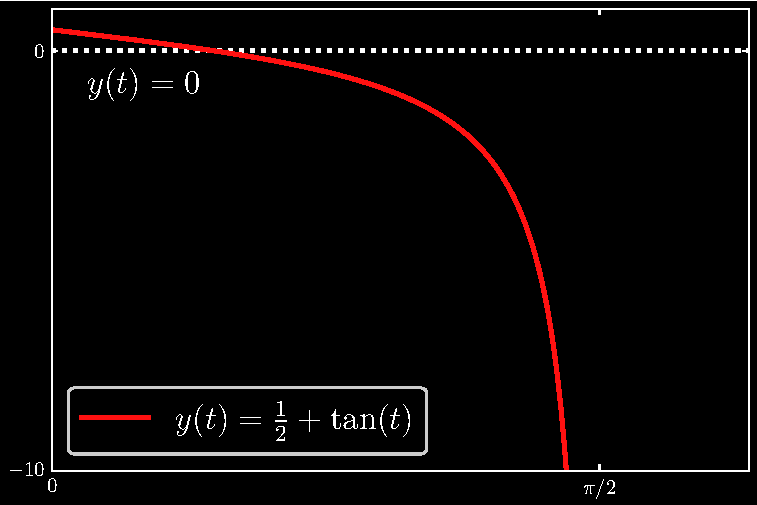
\includegraphics[width=1.0\textwidth]{chap1/sec1.7/chap1sec1.7ex13.eps}
\end{center}

\newpage
% QUESTION 14
\qs{1.7.14}{With \textbf{two partial fractions}, this is my preferred way to find \(\displaystyle{A = \frac{1}{r - s}}\), \(\displaystyle{B = \frac{1}{s - r}}\)
\[
	\boxed{\textbf{PF2}} \quad \bm{\frac{1}{\!\left( y - r \right) \!\left( y - s \right)} = \frac{1}{\!\left( y - r \right) \!\left( r - s \right) } + \frac{1}{\!\left( y - s \right) \!\left( s - r \right) }}	
\]
Check that equation: The common denominator on the right is \(\!\left( \bm{y - r} \right) \!\left( \bm{y - s} \right) \!\left( \bm{r - s} \right) \). The numerator should cancel the \(\bm{r - s}\) when you combine the two fractions.
\[
	\text{Separate } \frac{1}{y^{2} - 1} \text{ and } \frac{1}{y^{2} - y} \text{ into two fractions } \frac{A}{y - r} + \frac{B}{y - s}.
\]
\textit{Note} When \(y\) approaches \(r\), the left side of \textbf{PF2} has a blowup factor \(1 / \!\left( y - r \right) \). The other factor \(1 / \!\left( y - s \right) \) correctly approaches \(A = 1/ \!\left( r - s \right) \). So the right side \textbf{of PF2} needs the same blowup at \(y = r\). The first term \(A / \!\left( y - r \right) \) fits the bill.}

To solve PF2, write
\begin{alignat*}{3}
	\implies && \frac{1}{\!\left( y - r \right) \!\left( r - s \right) } + \frac{1}{\!\left( y - s \right) \!\left( s - r \right) } & = \frac{\!\left( y - s \right) - \!\left( y - r \right) }{\!\left( y - r \right) \!\left( y - s \right) \!\left( r - s \right) } \\
	&&  & = \frac{r - s}{\!\left( y - r \right) \!\left( y - s \right) \!\left( r - s \right) } \\ 
	&& & = \frac{1}{\!\left( y - r \right) \!\left( y - s \right) } 
\end{alignat*}

Given
\[
	\frac{1}{y^{2} - 1}
\]
we derive, with \(r = 1\) and \(s = -1\):

\begin{alignat*}{3}
	\implies && \frac{1}{y^{2} - 1} & = \frac{1}{\!\left( y - 1 \right) \!\left( y + 1 \right) } \\
	&& & = \frac{1}{2} \frac{1}{y - 1} - \frac{1}{2} \frac{1}{y + 1}  
\end{alignat*}

Given

\[
	\frac{1}{y^{2} - y}
\]

we derive, with \(r = 0\) and \(s = 1\):

\begin{alignat*}{3}
	\implies && \frac{1}{y^{2} - y} & = \frac{1}{y \!\left( y - 1 \right) } \\
	&& & = -\frac{1}{y} + \frac{1}{y - 1}  \\ 
\end{alignat*}

% QUESTION 15
\qs{1.7.15}{The \textbf{threshold equation} is the logistic equation backward in time:
\[
	-\frac{d y}{d t} = ay - by^{2} \quad \text{is the same as} \quad \frac{d y}{d t} = -ay + by^{2}
\]
Now \(Y = 0\) is the stable steady state. \(Y = a/b\) is the unstable state (why?). If \(y \!\left( 0 \right) \) is below the threshold \(a/b\) then \(y \!\left( t \right) \rightarrow 0\) and the species will die out.

Graph \(y \!\left( t \right) \) with \(y \!\left( 0 \right) < a/b\) (reverse \(S\)-curve). Then graph \(y \!\left( t \right) \) with \(y \!\left( 0 \right) > a/b\).}

Given the equation
\[
	-\frac{d y}{d t} = ay - by^{2}
\]
We let \(z = 1/y\), implying that
\[
	\frac{d z}{d t} = -\frac{1}{y^{2}} \frac{d y}{d t} 
\]
Thus we may rewrite our equation as
\[
	\frac{d z}{d t} = \frac{a}{y} - b = az - b
\]
and solve as follows:

\begin{alignat*}{3}
	\implies &&\int^{z \!\left( t \right) }_{z \!\left( 0 \right) } \frac{dz}{az - b}  & = \int^{t}_{0}  \, dt  \\
	\implies && \frac{1}{a} \left[ \ln\left( a z \!\left( t \right) - b \right) - \ln\left( a z \!\left( 0 \right) - b \right) \right]  & = t \\ 
	\implies && \frac{a z \!\left( t \right) - b}{a z \!\left( 0 \right) - b} & = e^{at} \\
	\implies && z \!\left( t \right) & = \left[ \!\left( a z \!\left( 0 \right) - b \right) e^{at} + b \right] \\
		 && & = z \!\left( 0 \right) e^{at} + \frac{b}{a} \!\left( 1 - e^{at} \right) 
\end{alignat*}
Now, define
\[
	\frac{d}{a} = z \!\left( 0 \right) - \frac{b}{a} = \frac{1}{y \!\left( 0 \right) - \frac{b}{a}}
\]
Then our equation for \(z \!\left( t \right) \) can be compactly written as
\[
	z \!\left( t \right) = \frac{de^{at} + b}{a}
\]
and thus, our equation for \(y \!\left( t \right) \) is
\[
	y \!\left( t \right) = \frac{a}{de^{at} + b}
\]
This is the complete derivation for the threshold equation, but intuitively, we need only realize that since the threshold equation is the logistic equation run backwards in time, we need only amend the solution to the logistic equation by taking the negative of time \(t\).

Now, if \(f \!\left( y \right) = -ay + by^{2}\), observe that
\[
	\frac{d f}{d y} = -a + 2by
\]
When \(Y = 0\) and \(Y = a/b\), we have, respectively,
\begin{alignat*}{3}
	\frac{d f}{d y}_{\!\left( Y = 0 \right) } & = - a < 0 && \quad \text{(stable)} \\
	\frac{d f}{d y}_{\!\left( Y = a/b \right) } & = a > 0 && \quad \text{(unstable)}
\end{alignat*}

Graphically, we have

\begin{center}
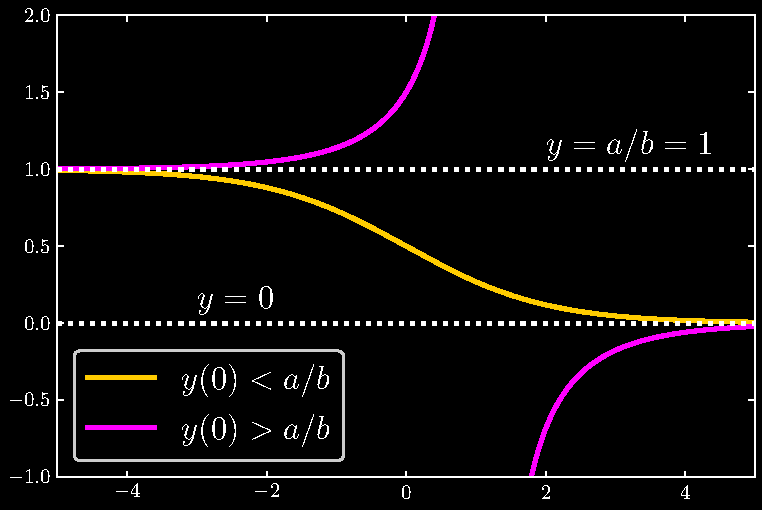
\includegraphics[width=1.0\textwidth]{chap1/sec1.7/chap1sec1.7ex15.eps}
\end{center}

\newpage
% QUESTION 16
\qs{1.7.16}{(Cubic nonlinearity) The equation \(y' = y \!\left( 1 - y \right) \!\left( 2 - y \right) \) has \textbf{three steady states}: \(Y = 0, 1, 2\). By computing the derivative \(df /dy\) at \(y = 0, 1, 2\), decide whether each of these states is stable or unstable.

Draw the \textit{stability line} for this equation, to show \(y \!\left( t \right) \) leaving the unstable \(Y\)'s. Sketch a graph that shows \(y \!\left( t \right) \) starting from \(y \!\left( 0 \right) = \frac{1}{2}\) and \(\frac{3}{2}\) and \(\frac{5}{2}\).}

Given \(f \!\left( y \right) = y \!\left( 1 - y \right) \!\left( 2 - y \right) \), we have
\begin{align*}
	\frac{d f}{d y} & = \!\left( 1 - y \right) \!\left( 2 - y \right) + y \left[ - \!\left( 2 - y \right) - \!\left( 1 - y \right)  \right] \\
			& = \!\left( 2 - 3y + y^{2} \right) + y \!\left( - 3 + 2y \right) \\
			& = \!\left( 2 - 3y + y^{2} \right) - 3y + 2y^{2} \\
			& = 2 - 6y + 3y^{2}  
\end{align*}
At the values \(y = 0, 1, 2\), we have
\begin{align*}
	\frac{d f}{d y}_{\!\left( y = 0 \right)} & = 2 \\
	\frac{d f}{d y}_{\!\left( y = 1 \right) } & = -1 \\ 
	\frac{d f}{d y}_{\!\left( y = 2 \right) } & = 2
\end{align*}

Therefore, \(Y = 1\) is a stable state, while \(Y = 0, 2\) are unstable.

\begin{center}
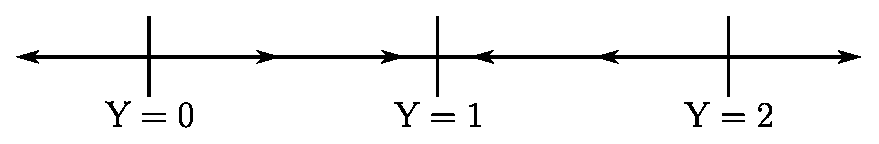
\includegraphics[width=1.0\textwidth]{chap1/sec1.7/c1s7q16.eps}
\end{center}

Using the stability line, we can capture the trajectories that beginning at different initial conditions takes us on. Starting from \(y \!\left( 0 \right) = 1/2 \), we can observe that \(y \!\left( t \right) \) approaches \(Y = 1\). So too when we begin at \(y \!\left( 0 \right) = 3/2\). However, when we commence at \(y \!\left( 0 \right) = 5/2\), \(y \!\left( t \right) \) diverges to \(+\infty\).

The equation really needs to be solved numerically. You can start to attempt an analytic approach by separable variables, and writing
\[
	\int^{y \!\left( t \right) }_{y \!\left( 0 \right) } \frac{dY}{Y \!\left( 1 - Y \right) \!\left( 2 - Y  \right) } = \int^{t}_{0}  \, dT
\]

Using partial fractions decomposition, the left-hand side is equal to
\[
	\int^{y \!\left( t \right) }_{y \!\left( 0 \right) } \!\left(  \frac{1}{2Y} + \frac{1}{1 - Y} - \frac{1}{2 \!\left( 2 - Y \right) }\right) \, dY 
\]
Multiply the integrand through by \(2\) (you'll see why in a moment). Enabling us to solve as follows:
\begin{align*}
	\left[ \ln\left( Y \right) - \ln\left( 1 - Y \right)^{2} - \ln\left( \!\left( 2 - Y \right) \right) \right]  \Biggr|^{y \!\left( t \right)}_{y \!\left( 0 \right) } & = \ln\left( \frac{y \!\left( t \right)}{\!\left( 1 - y \!\left( t \right)  \right)^{2} \!\left( 2 - y \!\left( t \right)  \right)} \right) \\ 
 	  & \ - \ln\left( \frac{y \!\left( 0 \right)}{\!\left( 1 - y \!\left( 0 \right)  \right)^{2} \!\left( 2 - y \!\left( 0 \right)  \right) } \right) \\ 
\end{align*}

Let the second term equal a constant \(-c\). On the right-hand side, we have
\[
	\int^{t}_{0} 2 \, dT = 2t 
\]
Equating both sides and exponentiating, we have
\[
	\frac{y \!\left( t \right) }{\!\left( 1 - y \!\left( t \right)  \right)^{2} \!\left( 2 - y \!\left( t \right)  \right) } = Ce^{2t}
\]
where \(C = e^{c}\). Let me know if you find a way to analytically proceed! 

\vspace{12pt}

% QUESTION 17
\qs{1.7.17}{\begin{enumerate}[label=(\alph*)]
	\item Find the steady states of the \textbf{Gompertz equation} \(dy / dt = y \!\left( 1 - \ln\left( y \right) \right) \).
	\item Show that \(z = \ln\left( y \right)\) satisfies the linear equation \(dz / dt = 1 - z\).
	\item The solution \(z \!\left( t \right) = 1 + e^{-t} \!\left( z \!\left( 0 \right) - 1 \right) \) gives what formula for \(y \!\left( t \right) \) from \(y \!\left( 0 \right) \)?
\end{enumerate}}

\textbf{(a)} The unambiguous steady state is \(Y = e\). Technically, the Gompertz equation \(f \!\left( y \right) = y \!\left( 1 - \ln\left( y \right) \right) \) is not defined at \(Y = 0\). It seems that the author considers \(Y = 0\) as a second steady state, however.

\vspace{12pt}

\textbf{(b)} From the definition of \(z\), we have
\[
	\frac{d z}{d t} = \frac{1}{y} \frac{d y}{d t} 
\]
By (a), we then derive
\[
	\frac{d z}{d t} = \frac{1}{y} \left[ y \!\left( 1 - \ln\left( y \right) \right)  \right] = 1 - \ln\left( y \right) = 1 - z 
\]

\vspace{12pt}

\textbf{(c)} We can rewrite this solution as
\[
	\ln\left( y \!\left( t \right)  \right) = 1 + e^{-t} \!\left( \ln\left( y \!\left( 0 \right) \right) - 1 \right) 
\]
Exponentiating yields
\[
	y \!\left( t \right) = \exp\left( 1 + e^{-t} \!\left( \ln\left( y \!\left( 0 \right)  \right) - 1 \right)  \right)
\]

Now, observe that	
\[
	\frac{d f}{d y} = - \ln\left( y \right)
\]
When \(Y = 0 + \epsilon \), for real, positive, and arbitrarily small \(\epsilon \), we have \(df / dy > 0\), so we have an unstable steady state. By contrast, when \(Y = e\), \(df / dy < 0\), a stable steady state. 

Suppose now that we have three cases: \(0 < y \!\left( 0 \right) < e\), \(y \!\left( 0 \right) = e\), and \(y \!\left( 0 \right) > e\). Our solution curves now look like

\begin{center}
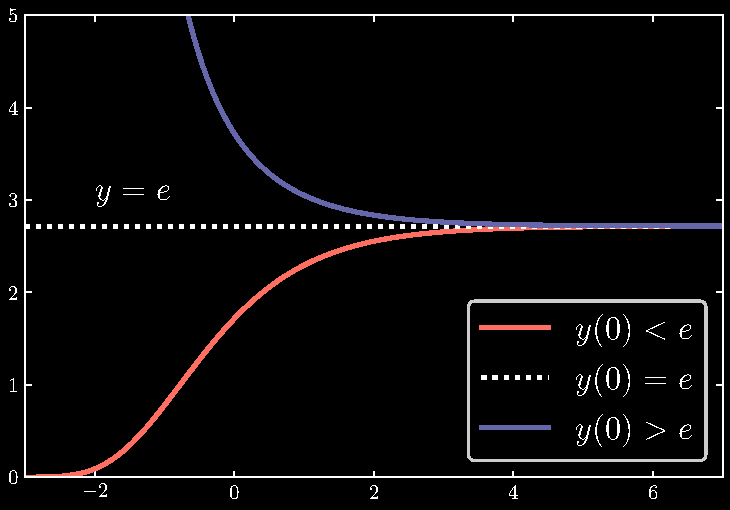
\includegraphics[width=1.0\textwidth]{chap1/sec1.7/chap1sec1.7ex17.eps}
\end{center}

% QUESTION 18
\qs{1.7.18}{Decide stability or instability for the steady states of

\begin{enumerate}[label=(\alph*)]
	\item \(dy/dt = 2 \!\left( 1 - y \right) \!\left( 1 - e^{y} \right) \)
	\item \(dy/dt = \!\left( 1 - y^{2} \right) \!\left( 4 - y^{2} \right) \)
\end{enumerate}}

\textbf{(a)} When \(Y = 0\) or \(Y = 1\), \(f \!\left( y \right) = 0\). Then differentiating gives us
\[
	\frac{d f}{d y} = - 2 \left[\!\left( 1 - y \right) e^{y} + \!\left( 1 - e^{y} \right)  \right]
\]
with
\begin{alignat*}{3}
	\frac{d f}{d y}_{\!\left( Y = 0 \right) } & = -2 < 0 & \text{(unstable)} \\
	\frac{d f}{d y}_{\!\left( Y = 1 \right) } & = -2 \!\left( 1 - e \right) > 0 & \text{(stable)} \\ 
\end{alignat*}

\textbf{(b)} When \(Y = \pm 1\) or \(Y = \pm 2\), \(f \!\left( y \right) = 0\). Then differentiating gives us
\[
	\frac{d f}{d y} = -2y \!\left( 5 - 2y^{2} \right)
\]
with
\begin{alignat*}{3}
	&\frac{d f}{d y}_{\!\left( Y = -1 \right) } && = 6 > 0 & \text{(unstable)}  \\
	&\frac{d f}{d y}_{\!\left( Y = 1 \right) } && = - 6 < 0 & \text{(stable)} \\ 
	&\frac{d f}{d y}_{\!\left( Y = -2 \right) } && = -12 < 0 & \text{(stable)} \\
	&\frac{d f}{d y}_{\!\left( Y = 2 \right) } && = 12 > 0 & \text{(unstable)}
\end{alignat*}

% QUESTION 19
\qs{1.7.19}{Stefan's Law of Radiation is \(dy/dt = K \!\left( M^{4} - y^{4} \right) \). It is unusual to see fourth powers. Find all real steady states and their stability. Starting from \(y \!\left( 0 \right) = M/2\), sketch a graph of \(y \!\left( t \right) \).}

We have \(f \!\left( y \right) = 0\) when \(y = \pm M, \pm iM\). We will only consider the real roots. The derivative of \(f \!\left( y \right) \) is
\[
	\frac{d f}{d y} = -4Ky^{3}
\]
which corresponds to
\begin{alignat*}{3}
	&\frac{d f}{d y}_{\!\left( Y = M \right) } && = -4KM^{3} < 0 & \text{(stable)} \\
	&\frac{d f}{d y}_{\!\left( Y = -M \right) } && = 4KM^{3} > 0 & \text{(unstable)} \\ 
\end{alignat*}

Beginning from \(y \!\left( 0 \right) = M/2\), \(y \!\left( t \right) \) approaches the stable steady state at \(Y = M\).

\vspace{12pt}

% QUESTION 20
\qs{1.7.20}{\(dy/dt = ay - y^{3}\) has how many steady states \(Y\) for \(a < 0\) and then \(a > 0\)? Graph those values \(Y \!\left( a \right) \) to see a \textit{pitchfork bifurcation}--new steady states suddenly appear as \(a\) passes zero. The graph of \(Y \!\left( a \right) \) looks like a pitchfork.}

\(\bm{a > 0}\): In the case where \(a\) is positive, we certainly have \(Y = 0\) as one steady state. Then we must also have \(Y = \pm \sqrt{a}\) as two other steady states. 

To derive the stability, calculate
\[
	\frac{d f}{d y} = a - 3y^{2}
\]
which corresponds to
\begin{alignat*}{3}
	&\frac{d f}{d y}_{\!\left( Y = -\sqrt{a} \right) } && = -2a < 0 & \text{(stable)} \\
	&\frac{d f}{d y}_{\!\left( Y = 0 \right) } && = a > 0 & \text{(unstable)} \\
	&\frac{d f}{d y}_{\!\left( Y = \sqrt{a} \right) } && = -2a < 0 & \text{(stable)}
\end{alignat*}

\(\bm{a < 0}\): When \(a\) is negative, we only have \(Y = 0\) as the steady state (as far as real roots go, and we stay in the realm of the reals for now).

Since \(a < 0\), \(df/dy = a < 0\) implies that the steady state is stable.

\begin{center}
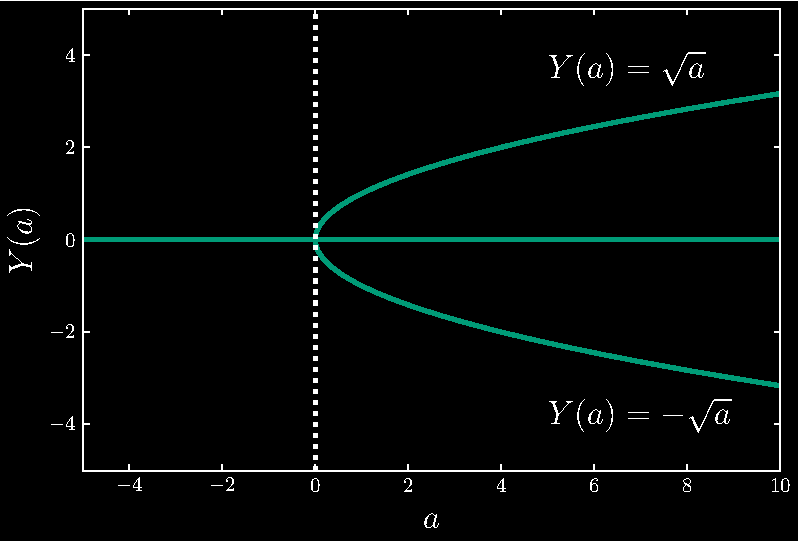
\includegraphics[width=1.0\textwidth]{chap1/sec1.7/chap1sec1.7ex20.eps}
\end{center}

% QUESTION 21
\qs{1.7.21}{(Recommended) The equation \(dy/dt = \sin y\) has \textbf{infinitely many steady states.} What are they and which ones are stable? Draw the stability line to show whether \(y \!\left( t \right) \) increases or decreases when \(y \!\left( 0 \right) \) is between two of the steady states.}

When \(f \!\left( y \right) = \sin y = 0\), we have \(Y = N \pi\) for all integer \(N\). Since \(df/dy = \cos y\), we have the cases:
\[
	Y \text{ is: }\begin{cases}
		\text{stable,} & N = 2k + 1, k \in \mathbb{Z}  \\
		\text{unstable,} & N = 2k, k \in \mathbb{Z} \\
	\end{cases}
\]

The stability line is pictured below:

\begin{center}
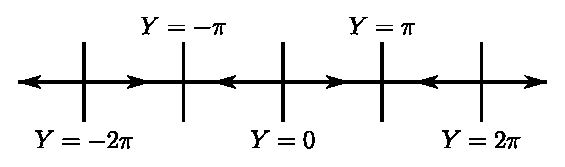
\includegraphics[width=1.0\textwidth]{chap1/sec1.7/c1s7q21.eps}
\end{center}

% QUESTION 22
\qs{1.7.22}{Change Problem 21 to \(dy/dt = \!\left( \sin y \right)^{2}\). The steady states are the same, but now the derivative of \(f \!\left( y \right) = \!\left( \sin y \right)^{2}\) is zero at all those states (because \(\sin y\) is zero). What will the solution actually do if \(y \!\left( 0 \right) \) is between two steady states?}

Here, we have
\[
	\frac{d f}{d y} = 2 \sin y \cos y = \sin 2y
\]
where for \(Y\) such that \(f \!\left( Y \right) = 0\), we also have \(df/dy = 0\). These \(Y\)'s are of the form
\[
	Y = n \pi 
\]

for all integers \(n\).

At the moment, it is ambiguous as to what type of stability each steady state is in. In fact, we call this \textbf{marginal stability}. To further investigate, we must go to the \textbf{second derivative} of \(f \!\left( y \right) \). To motivate this, let \(Y\) be our steady state, and let \(\epsilon \!\left( t \right) \) be some small perturbation around the steady state. Our \(y \!\left( t \right) \) is given by
\[
	y \!\left( t \right) = Y + \epsilon \!\left( t \right) 
\]
Differentiating both sides, taking into account that \(Y\) is a constant, we derive
\[
	y' \!\left( t \right) = \epsilon' \!\left( t \right) 
\]
And since \(y' \!\left( t \right) = f \!\left( y \right) \), we have
\[
	\epsilon' \!\left( t \right) = f \!\left( Y + \epsilon \!\left( t \right)  \right) 
\]
Using the Taylor series expansion, we may write
\[
	\epsilon' \!\left( t \right) = f \!\left( Y \right) + \epsilon f' \!\left( Y \right) + \epsilon^{2} f'' \!\left( Y \right) / 2 + \cdots 
\]
Note that the first two terms on the right side vanish, since \(f \!\left( Y \right) = f' \!\left( Y \right) = 0\). We should also ignore higher-order terms. That leaves us with the approximation
\[
	\epsilon' \!\left( t \right) \approx \epsilon^{2} f'' \!\left( Y \right) /2
\]
Now in this case, observe that
\[
	f'' \!\left( y \right) = 2 \left( \cos^{2}y - \sin^{2}y \right) = 2 \cos 2y
\]

We can conclude that for any of our aforementioned steady states \(Y\), which are of form \(n \pi \) for integers \(n\), it \textit{must} be the case that
\[
	f''\!\left( Y \right) > 0
\]
Moreover, since \(\epsilon^{2}\) is always positive irrespective of the value of \(\epsilon \!\left( t \right) \), we can now conclude that
\[
	\epsilon' \!\left( t \right) > 0
\]
Therefore, going back to the equality between \(y'\!\left( t \right) \) and \(\epsilon' \!\left( t \right) \), it immediately follows that
\[
	y'\!\left( t \right) > 0
\]
So for any perturbation \(\epsilon \!\left( t \right) \), we will have increasing \(y \!\left( t \right) \), meaning that \(y \!\left( t \right) \) will indefinitely move to successively higher steady states \(Y\).\footnote{\href{https://math.libretexts.org/Bookshelves/Differential_Equations/Differential_Equations_(Chasnov)/08\%3A_Nonlinear_Differential_Equations/8.01\%3A_Fixed_Points_and_Stability}{See this LibreText chapter on fixed points and stability here.}}

\vspace{12pt}

% QUESTION 23
\qs{1.7.23}{(\textit{Research project}) Find actual data on the US population in the years 1950, 1980, and 2010. What values of \(a\), \(b\), \(d\) in the solution formula (7) will fit these values? is the formula accurate at 2000, and what population does it predict for 2020 and 2100?

You could reset \(t = 0\) to the year 1950 and rescale time so that \(t = 3\) is 1980.}

Will return to this with some numerical methods.

\vspace{12pt}

% QUESTION 24
\qs{1.7.24}{If \(dy/dt = f \!\left( y \right) \), what is the limit \(y \!\left( \infty \right) \) starting from each point \(y \!\left( 0 \right) \)?

\begin{center}
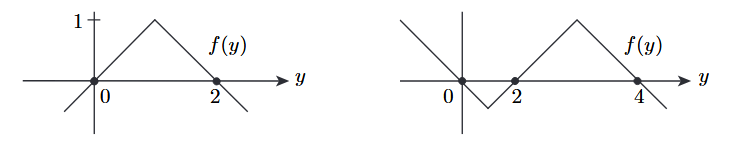
\includegraphics[width=1.0\textwidth]{chap1/sec1.7/c1s7q24.png}
\end{center}}

In the first graph, we have \(f \!\left( y \right) = 0\) when \(Y = 0\), \(2\). At these respective points, \(f'\!\left( y \right) > 0\) and \(f'\!\left( y \right) < 0\). Then \(Y = 0\) is an unstable steady state, while \(Y = 2\) is stable. As such, we have the cases
\[
	y \!\left( \infty \right) = \begin{cases}
		- \infty & y \!\left( 0 \right) < 0 \\
		2 & y \!\left( 0 \right) > 0  \\
	\end{cases}
\]
For the second graph, we have steady states at \(Y = 0\), \(2\), and \(4\). At each of those points, we have \(f'\!\left( y \right) < 0\), \(f'\!\left( y \right) > 0\), and \(f' \!\left( y \right) < 0\), respectively. These steady states are, in order, stable, unstable, and stable. We have the cases
\[
	y \!\left( \infty \right) = \begin{cases}
		0 & y \!\left( 0 \right) < 2 \\
		4 & y \!\left( 0 \right) > 2 \\
	\end{cases}
\]

% QUESTION 25
\qs{1.7.25}{
\begin{enumerate}[label=(\alph*)]
	\item Draw a function \(f \!\left( y \right) \) so that \(y \!\left( t \right) \) approaches \(y \!\left( \infty \right) = 3\) from every \(y \!\left( 0 \right) \).
	\item Draw \(f \!\left( y \right) \) so that \(y \!\left( \infty \right) = 4\) if \(y \!\left( 0 \right) > 0\) and \(y \!\left( \infty \right) = -2\) if \(y \!\left( 0 \right) < 0\).
\end{enumerate}}

\textbf{(a)} Consider the function
\[
	f \!\left( y \right) = 3 - y
\]
Then \(f \!\left( Y \right) = 0\) when \(Y = 3\), and \(df/dy = -1\) for all \(y\). Thus \(Y = 3\) is a stable steady state.

\begin{center}
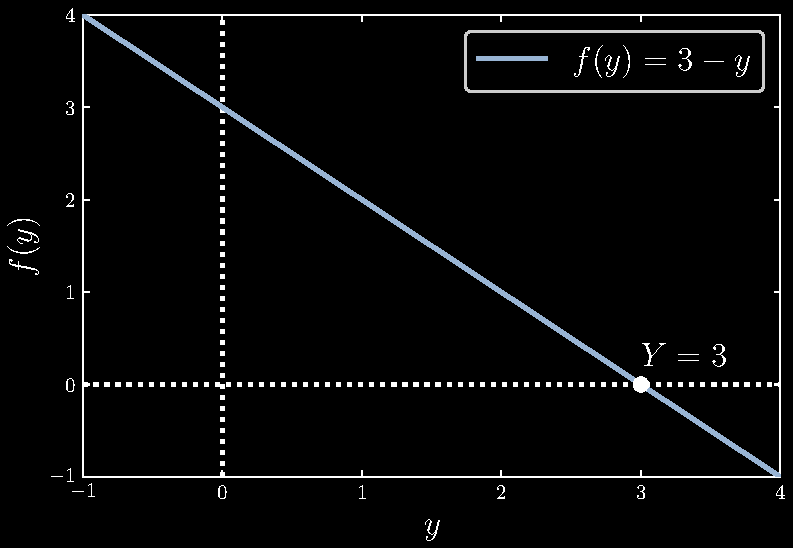
\includegraphics[width=1.0\textwidth]{chap1/sec1.7/chap1sec1.7ex25a.eps}
\end{center}

\textbf{(b)} Here, we must have \(Y = 4\) and \(Y = -2\) as stable steady states, and \(Y = 0\) as an unstable steady state. One approach is to define a piecewise function as follows:
\[
	f \!\left( y \right) = \begin{cases}
		-2 - y & y \le -1 \\
		y & -1 < y \le 2 \\
		4 - y & 2 < y \\
	\end{cases}
\]
\begin{center}
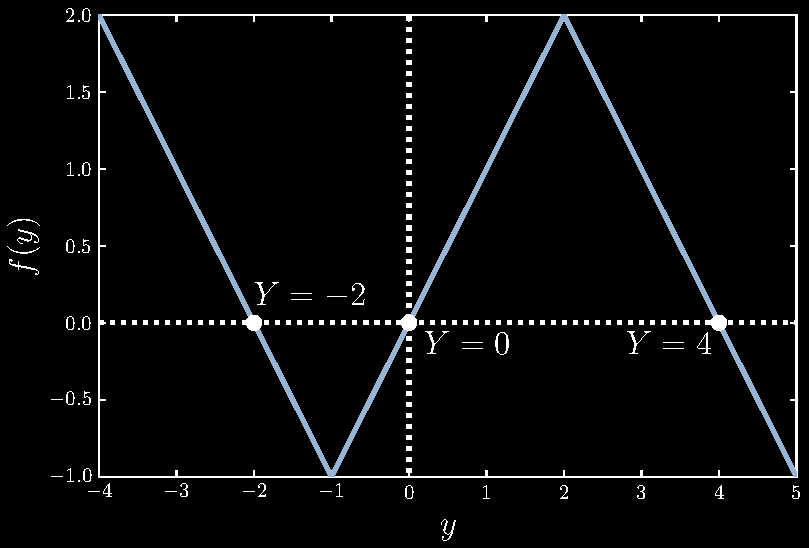
\includegraphics[width=1.0\textwidth]{chap1/sec1.7/chap1sec1.7ex25b.eps}
\end{center}

which is consistent with the stability of each of the steady states:
\begin{alignat*}{4}
	&\frac{d f}{d y}_{\!\left( Y = -2 \right) } && = & -1 \\
	&\frac{d f}{d y}_{\!\left( Y = 0 \right) } && = & 1 \\ 
	&\frac{d f}{d y}_{\!\left( Y = 4 \right) } && = & -1
\end{alignat*}

% QUESTION 26
\qs{1.7.26}{Which exponents \(n\) in \(dy/dt = y^{n}\) produce blowup \(y \!\left( T \right) = \infty\) in a finite time? You could separate the equation into \(dy/y^{n} = dt\) and integrate from \(y \!\left( 0 \right) = 1\).}

First consider the case that \(n = 1\). Then we have
\begin{alignat*}{3}
	\implies && \int^{y \!\left( t \right) }_{y \!\left( 0 \right) } \frac{dy}{y} & = \int^{t}_{0} \, dT \\
	\implies && \ln\left( y \!\left( t \right)  \right) - \ln\left( y \!\left( 0 \right)  \right) & = t \\ 
	\implies&& y \!\left( t \right) & = e^{t}
\end{alignat*}
which does \textbf{not} blowup to \(\infty\) in a finite time. In the general case, however, we have
\begin{alignat*}{3}
	\implies &&\int^{y \!\left( t \right) }_{y \!\left( 0 \right) } \frac{dy}{y^{n}} & = \int^{t}_{0}  \, dT  \\
	\implies &&-\frac{1}{n-1} \!\left( y^{-\!\left( n - 1 \right) } - 1 \right) & = t \\ 
	\implies&& y^{n-1} \!\left( t \right) & = \frac{1}{1 - \!\left( n - 1 \right) t} 
\end{alignat*}

where it is apparent that \(y \!\left( t \right) \) diverges to infinity at finite time for
\[
	T = \frac{1}{n - 1}
\]
We may conclude that for \(n > 1\), there exists a finite time \(T\) where \(y \!\left( t \right) \) diverges to infinity.

\vspace{12pt}

% QUESTION 27
\qs{1.7.27}{Find the steady states of \(dy/dt = y^{2} - y^{4}\) and decide whether they are stable, unstable, or one-sided stable. Draw a stability line to show the final value \(y \!\left( \infty \right) \) from each initial value \(y \!\left( 0 \right) \).}

Given \(f \!\left( y \right) = y^{2} - y^{4}\), we have \(Y = \pm 1\) and \(Y = 0\) corresponding to \(f \!\left( Y \right) = 0\).
\[
	f'\!\left( y \right) = 2y - 4y^{3}
\]
For \(Y = 1\), we have \(f'\!\left( Y = 1 \right) = -2 < 0\), a stable steady state. Conversely, for \(Y = -1\), we have \(f' \!\left( Y = -1 \right) = 2 > 0\), an unstable steady state.

The remaining steady state at \(Y = 0\) is somewhat problematic. Following the logic of question 1.7.22, we take the second derivative of \(f \!\left( y \right) \) to get
\[
	f''\!\left( y \right) = 2 - 12y^{2}
\]
which, for \(f''\!\left( Y = 0 \right) = 2 > 0\), implies that for any perturbation \(\epsilon \!\left( t \right) \), we have \(\epsilon' \!\left( t \right) > 0\), implying that \(y'\!\left( t \right) > 0\), and thus increasing \(y \!\left( t \right) \). Finally, we can conclude that the stability line looks like:

\begin{center}
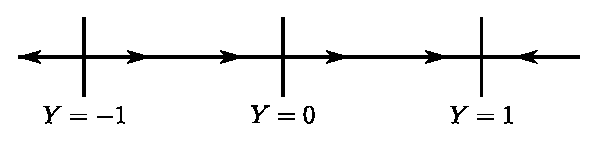
\includegraphics[width=1.0\textwidth]{chap1/sec1.7/c1s7q27.eps}
\end{center}

% QUESTION 28
\qs{1.7.28}{For an autonomous equation \(y' = f \!\left( y \right) \), why is it impossible for \(y \!\left( t \right) \) to be increasing at one time \(t_{1}\) and decreasing at another time \(t_{2}\)?}

The crux of the explanation has to do with \textbf{steady states}. First consider the case where either \(y \!\left( 0 \right) \) lies above or below a stable steady state. We can think of a stable steady state as a kind of ``attractor''; a magnet or celestial body that pulls a point particle onto it. 

In this case, the point particle moves \textbf{monotonically} in \textbf{one} direction towards the stable steady state, so we cannot have \(y'\!\left( t_{1} \right) > 0\) and \(y'\!\left( t_{2} \right) < 0\), \(t_{1} \neq t_{2}\), simultaneously.

In the case where there is no stable steady state (such as in the overharvesting case), \(y \!\left( t \right) \) diverges to \(-\infty\) -- once again, monotonically. 

\newpage
\subsection{\textsf{1.8 - Separable Equations and Exact Equations}}
% QUESTION 1
\qs{1.8.1}{Finally we can solve the example \(dy/dt = y^{2}\) in Section 1.1 of this book.

Start from \(y \!\left( 0 \right) = 1\). Then \(\displaystyle{\int^{y}_{1} \frac{dy}{y^{2}} = \int^{t}_{0}  \, dt  }\). Notice the limits on \(y\) and \(t\). Find \(y \!\left( t \right) \).}

Solve as follows:

\begin{alignat*}{3}
	\implies &&\int^{y}_{1} \frac{dy}{y^{2}} & = \int^{t}_{0}  \, dt  \\
	\implies && -y^{-1} + 1 & = t \\ 
	\implies && y \!\left( t \right) & = \frac{1}{1 - t}
\end{alignat*}

% QUESTION 2
\qs{1.8.2}{Start the same equation \(dy/dt = y^{2}\) from any value \(y \!\left( 0 \right) \). At what time \(t\) does the solution blow up? For which starting values \(y \!\left( 0 \right) \) does it never blow up?}

Let \(y \!\left( 0 \right) = a\). Then we have
\[
	y \!\left( t \right) = \frac{1}{a^{-1} - t} = \frac{a}{1 - at}
\]

In general, \(y \!\left( t \right) \) blows up at \(t = 1/a\). Suppose that \(a \le 0\). Then the denominator \(1 - at\) never approaches zero, so \(y \!\left( t \right) \) never diverges to infinity.

\vspace{12pt}

% QUESTION 3
\qs{1.8.3}{Solve \(dy/dt = a \!\left( t \right) y\) as a separable equation starting from \(y \!\left( 0 \right) = 1\), by choosing \(f \!\left( y \right) = 1/y\). This equation gave the growth factor \(G \!\left( 0,t \right) \) in Section 1.6.}

Solve as follows:

\begin{alignat*}{3}
	\implies &&\int^{y \!\left( t \right) }_{1} \frac{dy}{y} & = \int^{t}_{0} a \!\left( t \right)  \, dt  \\
	\implies && \ln\left( y \!\left( t \right)  \right) & = \int^{t}_{0} a \!\left( t \right)  \, dt  \\ 
	\implies && y \!\left( t \right) & = e^{\int^{t}_{0} a \!\left( t \right)  \, dt }
\end{alignat*}

% QUESTION 4
\qs{1.8.4}{Solve these separable equations starting from \(y \!\left( 0 \right) = 0\):

\begin{enumerate}[label=(\alph*)]
	\item \(\displaystyle{\frac{d y}{d t} = ty}\)
	\item \(\displaystyle{\frac{d y}{d t} = t^{m}y^{n}}\)
\end{enumerate}}

Ignore the initial condition. We cannot have it at zero.

\textbf{(a)}
\begin{alignat*}{3}
	\implies &&\int^{y \!\left( t \right) }_{0} \frac{dy}{y} & = \int^{t}_{0} t \, dt  \\
	\implies && \ln\left( y \!\left( t \right)  \right) - \ln\left( y \!\left( 0 \right)  \right) & = \frac{t^{2}}{2} \\
	\implies && y \!\left( t \right) & = y \!\left( 0 \right) e^{t^{2}/2}
\end{alignat*}

\textbf{(b)} 
\begin{alignat*}{3}
	\implies &&\int^{y \!\left( t \right) }_{y \!\left( 0 \right) } \frac{dy}{y^{n}} & = \int^{t}_{0} t^{m} \, dt  \\
	\implies && -\frac{1}{n-1} \!\left(  y \!\left( t \right)^{-\!\left( n - 1 \right) } - y \!\left( 0 \right)^{-\!\left( n - 1 \right) }\right) & = \frac{1}{m + 1}t^{m + 1} \\ 
	\implies && y \!\left( t \right)^{-\!\left( n - 1 \right) } & = y \!\left( 0 \right)^{-\!\left( n - 1 \right) } - \frac{n - 1}{m + 1}t^{m + 1} \\
	\implies && y \!\left( t \right) & = \left[ y \!\left( 0 \right)^{-\!\left( n - 1 \right) } - \frac{n - 1}{m + 1}t^{m + 1} \right]^{\frac{1}{1 - n}} 
\end{alignat*}

% QUESTION 5
\qs{1.8.5}{Solve \(\displaystyle{\frac{d y}{d t} = a \!\left( t \right) y^{2} = \frac{a \!\left( t \right) }{1/y^{2}}}\) as a separable equation starting from \(y \!\left( 0 \right) = 1\).}

Solve as follows:

\begin{alignat*}{3}
	\implies && \int^{y \!\left( t \right) }_{y \!\left( 0 \right) } \frac{dy}{y^{2}} & = \int^{t}_{0} a \!\left( t \right)  \, dt  \\
	\implies && -\!\left( y \!\left( t \right)^{-1} - y \!\left( 0 \right)^{-1} \right) & = \int^{t}_{0} a \!\left( t \right)  \, dt  \\ 
	\implies && y \!\left( t \right)  & = \left[ y \!\left( 0 \right)^{-1} - \int^{t}_{0} a \!\left( t \right)  \, dt  \right]^{-1} \\
		 && & = \left[ 1 - \int^{t}_{0} a \!\left( t \right)  \, dt  \right]^{-1}
\end{alignat*}

% QUESTION 6
\qs{1.8.6}{The equation \(\displaystyle{\frac{d y}{d t} = y + t}\) is not separable or exact. But it is linear and \(y = \) \underline{\qquad}.}

Use an integrating factor: \(e^{-t}\).

\begin{alignat*}{3}
	\implies && \!\left( e^{-t}y \right)' & = te^{-t} \\
	\implies && e^{-t} y \!\left( t \right) - y \!\left( 0 \right)  & = \int^{t}_{0} te^{-t} \, dt  \\ 
	\implies && y \!\left( t \right) & = e^{t} y \!\left( 0 \right) - \!\left( 1 + t - e^{t} \right) 
\end{alignat*}

% QUESTION 7
\qs{1.8.7}{The equation \(\displaystyle{\frac{d y}{d t} = \frac{y}{t}}\) has the solution \(y = At\) for every constant \(A\). Find this solution by separating \(f = 1/y\) from \(g = 1/t\). Then integrate \(dy/y = dt/t\). Where does the constant \(A\) come from?}

Solve as follows:

\begin{alignat*}{3}
	\implies && \int^{y \!\left( t \right) }_{y \!\left( 0 \right) } \frac{dy}{y} & = \int^{t}_{t_{0}} \frac{dt}{t}  \\
	\implies && \ln\left( y \!\left( t \right)  \right) - \ln\left( y \!\left( 0 \right)  \right) & = \ln\left( t \right) - \ln\left( t_{0} \right) \\
	\implies && y \!\left( t \right) & = \frac{y \!\left( 0 \right) }{t_{0}} t
\end{alignat*}

Lastly, define \(A = y \!\left( 0 \right) / t_{0}\).

\vspace{12pt}

% QUESTION 8
\qs{1.8.8}{For which number \(A\) is \(\displaystyle{\frac{d y}{d t} = \frac{ct - ay}{At + by}}\) an exact equation? For this \(A\), solve the equation by finding a suitable function \(F \!\left( y,t \right) + C \!\left( t \right) \).}

The exactness condition is met when
\[
	\frac{\partial g}{\partial y} = -\frac{\partial f}{\partial t} 
\]
Here, we are given
\[
	g \!\left( y, t \right) = ct - ay \quad \text{and} \quad f \!\left( y,t \right) = At + by
\]
Thus we must have
\[
	\frac{\partial g}{\partial y} = -a = -A = -\frac{\partial f}{\partial t} 
\]
Implying that \(A = a\). First, we find \(F \!\left( y,t \right) + C \!\left( t \right) \):
\[
	\int \!\left( at + by \right)  \, dy  = aty + \frac{by^{2}}{2} + C \!\left( t \right)
\]

Next, we differentiate with respect to \(t\) to find
\[
	\frac{\partial }{\partial t} \!\left( aty + \frac{by^{2}}{2} + C \!\left( t \right)  \right) = ay - ct
\]
Implying that
\[
	C \!\left( t \right) = -\frac{ct^{2}}{2}
\]
Thus the equation is solved by
\[
	F \!\left( y,t \right) + C \!\left( t \right) = aty + \frac{by^{2}}{2} - \frac{ct^{2}}{2} = \text{constant}
\]

% QUESTION 9
\qs{1.8.9}{Find a function \(y \!\left( t \right) \) different from \(y = t\) that has \(dy/dt = y^{2}/t^{2}\).}

Solve as follows:

\begin{alignat*}{3}
	\implies &&\int \frac{dy}{y^{2}} & = \int \frac{dt}{t^{2}} \\
	\implies && -y^{-1} & = -t^{-1} + C \\ 
	\implies && y \!\left( t \right) & = \frac{t}{1 + tC}
\end{alignat*}

The given example has \(C = 0\). Simply choose any nonzero \(C\). More concretely, the choice of \(C\) is given by

\begin{alignat*}{3}
	\implies &&\int^{y \!\left( t \right) }_{y \!\left( 0 \right) } \frac{dy}{y^{2}} & = \int^{t}_{t \!\left( 0 \right) } \frac{dt}{t^{2}}  \\
	\implies && -y \!\left( t \right)^{-1} + y \!\left( 0 \right)^{-1} & = -t^{-1} + t \!\left( 0 \right)^{-1} \\ 
	\implies && y \!\left( t \right) & = \left[ t^{-1} + y \!\left( 0 \right)^{-1} - t \!\left( 0 \right)^{-1} \right]^{-1} \\
		 && & = \frac{t}{1 + \!\left( y \!\left( 0 \right)^{-1} - t \!\left( 0 \right)^{-1} \right) t}
\end{alignat*}

where \(C\) is given by
\[
	C = y \!\left( 0 \right)^{-1} - t \!\left( 0 \right)^{-1}
\]

% QUESTION 10
\qs{1.8.10}{These equations are separable after factoring the right hand sides:
\[
	\text{Solve} \quad \frac{d y}{d t} = e^{y + t} \quad \text{and} \quad \frac{d y}{d t} = yt + y + t + 1
\]}

\textbf{(i)} Decompose the right hand side into \(e^{y}e^{t}\). Solve as follows:

\begin{alignat*}{3}
	\implies &&\int \frac{dy}{e^{y}} & = \int e^{t} \, dt \\
	\implies && -e^{-y} & = e^{t} + C \\ 
	\implies && y \!\left( t \right) & = -\ln\left( -e^{t} + C \right) 
\end{alignat*}

\textbf{(ii)} Factor the right hand side into \(\!\left( y + 1 \right) \!\left( t + 1 \right) \). Then solve as follows:

\begin{alignat*}{3}
	\implies &&\int \frac{dy}{y + 1} & = \int \!\left( t + 1 \right) \, dt \\
	\implies && \ln\left( y + 1 \right) & = \frac{t^{2}}{2} + t + C  \\ 
	\implies && y \!\left( t \right) & = \exp\left( \frac{t^{2}}{2} + t + C \right) - 1 
\end{alignat*}

% QUESTION 11
\qs{1.8.11}{These equations are linear and separable: Solve \(\displaystyle{\frac{d y}{d t} = \!\left( y + 4 \right) \cos t}\) and \(\displaystyle{\frac{d y}{d t} = ye^{t}}\).}

We write
\begin{alignat*}{3}
	\implies && \int^{y \!\left( t \right) }_{y \!\left( 0 \right) } \frac{dy}{y + 4} & = \int^{t}_{0} \cos\left( t \right) \, dt  \\
	\implies && \ln\left( \frac{y \!\left( t \right) + 4}{y \!\left( 0 \right) + 4} \right)& = \sin\left( t \right) \\ 
	\implies && y \!\left( t \right) & = \!\left( y \!\left( 0 \right) + 4 \right) e^{\sin\left( t \right)} - 4
\end{alignat*}

And for the second equation
\begin{alignat*}{3}
	\implies && \int^{y \!\left( t \right) }_{y \!\left( 0 \right) } \frac{dy}{y}  & = \int^{t}_{0} e^{t} \, dt  \\
	\implies && \ln\left( \frac{y \!\left( t \right) }{y \!\left( 0 \right) } \right) & = e^{t} - 1 \\
	\implies && y \!\left( t \right) & = y \!\left( 0 \right) e^{e^{t} - 1}
\end{alignat*}

% QUESTION 12
\qs{1.8.12}{Solve these three separable equations starting from \(y \!\left( 0 \right) = 1\):
\begin{enumerate}[label=(\alph*)]
	\item \(\frac{d y}{d t} = -4ty\)
	\item \(\frac{d y}{d t} = ty^{3}\)
	\item \(\!\left( 1 + t \right) \frac{d y}{d t} = 4y\)
\end{enumerate}}

Solve as follows:

(a) 

\begin{alignat*}{3}
	\implies && \int^{y \!\left( t \right) }_{y \!\left( 0 \right) } \frac{dy}{y}  & = -4 \int^{t}_{0} t \, dt  \\
	\implies && \ln\left( \frac{y \!\left( t \right) }{y \!\left( 0 \right) } \right) & = -4 \!\left( \frac{t^{2}}{2} \right)  \\ 
	\implies && y \!\left( t \right)  & = y \!\left( 0 \right) e^{-2t^{2}} \\
		 && & = e^{-2t^{2}}
\end{alignat*}

(b) 

\begin{alignat*}{3}
	\implies && \int^{y \!\left( t \right) }_{y \!\left( 0 \right) } \frac{dy}{y^{3}}  & = \int^{t}_{0} t \, dt  \\
	\implies && -\frac{1}{2} y \!\left( t \right)^{-2} + \frac{1}{2} y \!\left( 0 \right)^{-2} & = \frac{t^{2}}{2} \\ 
	\implies && y \!\left( t \right)^{-2} & = y \!\left( 0 \right)^{-2} - t^{2} \\
	\implies && y \!\left( t \right) & = \frac{y \!\left( 0 \right)}{\left[ 1 - \!\left( y \!\left( 0 \right)t \right)^{2} \right]^{1/2}} \\
		 && & = \frac{1}{\left[ 1 - \!\left( y \!\left( 0 \right) t \right)^{2} \right]^{1/2} }
\end{alignat*}

(c)

\begin{alignat*}{3}
	\implies && \int^{y \!\left( t \right) }_{y \!\left( 0 \right) } \frac{dy}{y}  & = 4 \int^{t}_{0} \!\left( 1 + t \right)  \, dt  \\
	\implies && \ln\left( \frac{y \!\left( t \right) }{y \!\left( 0 \right) } \right) & = 4\!\left( t + \frac{t^{2}}{2} \right)  \\ 
	\implies && y \!\left( t \right) & = y \!\left( 0 \right) e^{4t + 2t^{2}} \\
		 && & = e^{4t + 2t^{2}}
\end{alignat*}

\newpage

\textbf{Test the exactness condition \(\bm{\partial g / \partial y = -\partial f / \partial t}\) and solve Problems 13-14.}

\vspace{12pt}

% QUESTION 13
\qs{1.8.13}{
\begin{enumerate}[label=(\alph*)]
	\item \(\displaystyle{\frac{d y}{d t} = \frac{-3t^{2} - 2y^{2}}{4ty + 6y^{2}}}\)
	\item \(\displaystyle{\frac{d y}{d t} = -\frac{1 + ye^{ty}}{2y + te^{ty}}}\)
\end{enumerate}}

(a) The exactness condition is
\[
	\frac{\partial g}{\partial y} = -4y = -\frac{\partial f}{\partial t}  
\]

Next, we integrate \(f \!\left( y,t \right) \) with respect to \(y\):
\[
	\int \!\left( 4ty + 6y^{2} \right) \, dy = 2ty^{2} + 2y^{3} + C \!\left( t \right) 
\]
and differentiate \(F \!\left( y, t \right) + C \!\left( t \right) \) with respect to \(t\):
\[
	\frac{\partial }{\partial t} \!\left( F \!\left( y,t \right) + C \!\left( t \right)  \right) = 2y^{2} + C' \!\left( t \right) 
\]
which itself is equal to \(-g \!\left( y, t \right) \), implying that
\[
	C' \!\left( t \right) = 3t^{2} \quad \implies \quad C \!\left( t \right) = t^{3}
\]
Therefore, \(dy/dt\) is solved by
\[
	F \!\left( y,t \right) + C \!\left( t \right) = 2ty^{2} + 2y^{3} + t^{3}
\]

(b) The exactness condition is
\[
	\frac{\partial g}{\partial y} = -e^{ty} - tye^{ty} = -\frac{\partial f}{\partial t} 
\]
Next, we integrate \(f \!\left( y,t \right) \) with respect to \(y\):
\[
	\int \!\left( 2y + te^{ty} \right) \, dy = y^{2} + e^{ty} + C \!\left( t \right) 
\]
and differentiate \(F \!\left( y,t \right) + C \!\left( t \right) \) with respect to \(t\):
\[
	\frac{\partial }{\partial t} \!\left( F \!\left( y, t \right) + C \!\left( t \right)  \right) = ye^{ty} + C'\!\left( t \right)  
\]
which itself is equal to \(-g \!\left( y,t \right) \), implying that
\[
	C'\!\left( t \right) = 1 \quad \implies \quad C \!\left( t \right) = t
\]
Therefore, \(dy/dt\) is solved by
\[
	F \!\left( y,t \right) + C \!\left( t \right) = y^{2} + e^{ty} + t
\]

% QUESTION 14
\qs{1.8.14}{
\begin{enumerate}[label=(\alph*)]
	\item \(\displaystyle{\frac{d y}{d t} = \frac{4t - y}{t - 6y}}\)
	\item \(\displaystyle{\frac{d y}{d t} = - \frac{3t^{2} + 2y^{2}}{4ty + 6y^{2}}}\)
\end{enumerate}}

(a) The exactness condition is
\[
	\frac{\partial g}{\partial y} = -1 = \frac{\partial f}{\partial t} 
\]
Next, we integrate \(f \!\left( y,t \right) \) with respect to \(y\):
\[
	\int \!\left( t - 6y \right) \, dy = ty - 3y^{2} + C \!\left( t \right) 
\]
and differentiate \(F \!\left( y,t \right) + C \!\left( t \right) \) with respect to \(t\):
\[
	\frac{\partial }{\partial t} \!\left( F \!\left( y,t \right) + C \!\left( t \right)  \right) = y + C'\!\left( t \right) 
\]
which itself is equal to \(-g \!\left( y,t \right) \), implying that
\[
	C'\!\left( t \right) = -4t \quad \implies \quad C \!\left( t \right) = -2t^{2}
\]
Therefore, \(dy/dt\) is solved by
\[
	F \!\left( y,t \right) + C \!\left( t \right) = ty - 3y^{2} - 2t^{2}
\]
(b) The exactness condition is
\[
	\frac{\partial g}{\partial y} = -4y = -\frac{\partial f}{\partial t} 
\]
Next, we integrate \(f \!\left( y,t \right) \) with respect to \(y\):
\[
	\int \!\left( 4ty + 6y^{2} \right) \, dy = 2ty^{2} + 2y^{3} + C \!\left( t \right) 
\]
and differentiate \(F \!\left( y,t \right) + C \!\left( t \right) \) with respect to \(t\):
\[
	\frac{\partial }{\partial t} \!\left( F \!\left( y,t \right) + C \!\left( t \right)  \right) = 2y^{2} + C'\!\left( t \right)  
\]
which itself is equal to \(-g \!\left( y,t \right) \), implying that
\[
	C'\!\left( t \right) = 3t^{2} \quad \implies \quad C \!\left( t \right) = t^{3}
\]
Therefore, \(dy/dt\) is solved by
\[
	F \!\left( y,t \right) + C \!\left( t \right) = 2ty^{2} + 2y^{3} + t^{3}
\]
% QUESTION 15
\qs{1.8.15}{Show that \(\displaystyle{\frac{d y}{d t} = -\frac{y^{2}}{2ty}}\) is exact but the same equation \(\displaystyle{\frac{d y}{d t} = -\frac{y}{2t}}\) is not exact. Solve both equations. (This problem suggests that many equations become exact when multiplied by an integrating factor.)}

In the first case, we have \(g \!\left( y,t \right) = -y^{2}\) and \(f \!\left( y,t \right) = 2ty\). Then
\[
	\frac{\partial g}{\partial y} = -2y = -\frac{\partial f}{\partial t} 
\]
In the second case, \(g \!\left( y,t \right) = -y\) and \(f \!\left( y,t \right) = 2t\), establishing
\[
	\frac{\partial g}{\partial y} = -1 \neq -2 = -\frac{\partial f}{\partial t} 
\]
We solve the first equation as follows: first integrate \(f \!\left( y,t \right) \) with respect to \(y\):
\[
	\int 2ty \, dy = ty^{2}	+ C \!\left( t \right) 
\]
and then differentiate with respect to \(t\):
\[
	\frac{\partial }{\partial t} \!\left( F \!\left( y,t \right) + C \!\left( t \right)  \right) = y^{2} + C'\!\left( t \right) 
\]
which itself is equal to \(-g \!\left( y,t \right) \), allowing us to deduce
\[
	C'\!\left( t \right) = 0 \quad \implies C \!\left( t \right) = c
\]
where \(c\) is a constant. Then the equation is solved by
\[
	F \!\left( y,t \right) + C \!\left( t \right) = ty^{2} + c
\]
The second equation is separable, so we write
\begin{alignat*}{3}
	\implies && \int^{y \!\left( t \right) }_{y \!\left( 0 \right) } \frac{dy}{y}  & = -\int^{t}_{t \!\left( 0 \right) } \frac{dt}{2t}  \\
	\implies && \ln\left( \frac{y \!\left( t \right) }{y \!\left( 0 \right) } \right) & = -\frac{1}{2} \ln\left( \frac{t}{t \!\left( 0 \right) } \right) \\
	\implies && y \!\left( t \right) & = y \!\left( 0 \right) \!\left( \frac{t}{t \!\left( 0 \right) } \right)^{-1/2}
\end{alignat*}

\newpage

% QUESTION 16
\qs{1.8.16}{Exactness is really the condition to solve two equations with the same function \(H \!\left( t,y \right) \):
\[
	\frac{\partial H}{\partial y} = f \!\left( t,y \right) \quad \text{and} \quad \frac{\partial H}{\partial t} = - g \!\left( t,y \right) \quad \text{can be solved if} \quad \frac{\partial f}{\partial t} = - \frac{\partial g}{\partial y}  
\]
Take the \(t\) derivative of \(\partial H / \partial y\) and the \(y\) derivative of \(\partial H / \partial t\) to show that exactness is \textit{necessary}. It is also \textit{sufficient} to guarantee that a solution \(H\) will exist.}

We have
\[
	\frac{d }{d t} \frac{\partial H}{\partial y} = \frac{\partial f}{\partial t} \!\left( t,y \right)  \quad \text{and} \quad \frac{d }{d y} \frac{\partial H}{\partial t} = - \frac{\partial g}{\partial y} \!\left( t,y \right) 
\]
Exactness, then, is the condition where
\[
	\frac{d }{d t} \frac{\partial H}{\partial y} = \frac{d }{d y} \frac{\partial H}{\partial t} 
\]

% QUESTION 17
\qs{1.8.17}{The linear equation \(\displaystyle{\frac{d y}{d t} = aty + q }\) is not exact or separable. Multiply by the integrating factor \(e^{-\int at \, dt}\) and solve the equation starting from \(y \!\left( 0 \right) \).}

Write \(e^{-\int at \, dt} = e^{-at^{2}/2}\). Then
\begin{alignat*}{3}
	\implies && e^{-at^{2}/2} \frac{d y}{d t}  & = e^{-at^{2}/2} aty + e^{-at^{2}/2} q  \\
	\implies && \!\left( e^{-at^{2}/2} y \right)'  & = e^{-at^{2}/2}q \\ 
	\implies && e^{-at^{2}/2} y \!\left( t \right) - y \!\left( 0 \right)  & = q\int^{t}_{0} e^{-at^{2}/2}  \, dt  \\
	\implies && y \!\left( t \right) & = e^{at^{2}/2} y \!\left( 0 \right) + q e^{at^{2}/2} \int^{t}_{0} e^{-at^{2}/2} \, dt  
\end{alignat*}

\textbf{Second order equations \(\bm{F \!\left( t,y,y',y'' \right) = 0}\) involve the second derivative \(\bm{y''}\). This reduces to a first order equation for \(\bm{y'}\) (not \(\bm{y}\)) in two important cases:}

\begin{enumerate}[label=\Roman*.]
	\item When \(y\) is missing in \(F\), set \(y' = v\) and \(y'' = v'\). Then \(\bm{F \!\left( t, v, v' \right) = 0}\).
	\item When \(t\) is missing in \(F\), set \(\displaystyle{y'' = \frac{d v}{d t} = \frac{d v}{d y} \frac{d y}{d t} = v \frac{d v}{d y} }\). 

	Then \(\bm{F \!\left( y, v, v \frac{d v}{d y}  \right) = 0}\).
\end{enumerate}

See the website for \textbf{reduction of order} when one solution \(y \!\left( t \right) \) is known. 

% QUESTION 18
\qs{1.8.18}{(\(y\) is missing) Solve these differential equations for \(v = y'\) with \(v \!\left( 0 \right) = 1\). Then solve for \(y\) with \(y \!\left( 0 \right) = 0 \).

\begin{enumerate}[label=(\alph*)]
	\item \(y'' + y' = 0\)
	\item \(2ty'' - y' = 0\).
\end{enumerate}}

(a) We have
\[
	v' + v = 0
\]
which implies
\begin{alignat*}{3}
	\implies && \int^{v \!\left( t \right) }_{v \!\left( 0 \right) } \frac{dv }{v} & = -\int^{t}_{0}  \, dt  \\
	\implies && \ln\left( \frac{v \!\left( t \right) }{v \!\left( 0 \right) } \right) & = -t \\ 
	\implies && v \!\left( t \right) & = e^{-t} \\
	\implies && y'\!\left( t \right) & = e^{-t} \\
	\implies && \frac{d y}{d t} & = e^{-t} \\
	\implies && \int^{y \!\left( t \right) }_{y \!\left( 0 \right) }  \, dy & = \int^{t}_{0} e^{-t} \, dt \\
	\implies && y \!\left( t \right) & = 1 - e^{-t}
\end{alignat*}

(b) We have
\[
	2tv' - v = 0
\]
which implies
\begin{alignat*}{3}
	\implies && \int^{v \!\left( t \right) }_{v \!\left( 0 \right) } \frac{dv }{v} & = \int^{t}_{t \!\left( 0 \right) } \frac{dt}{2t} \\
	\implies && \ln\left( v \!\left( t \right)  \right) & = \frac{1}{2} \ln\left( \frac{t}{t \!\left( 0 \right) } \right) \\ 
	\implies && v \!\left( t \right) & = \!\left( \frac{t}{t \!\left( 0 \right) } \right)^{1/2} \\
	\implies && \frac{d y}{d t} & = \!\left( \frac{t}{t \!\left( 0 \right) } \right)^{1/2} \\
	\implies && \int^{y \!\left( t \right) }_{y \!\left( 0 \right) }  \, dy & = \frac{1}{t \!\left( 0 \right)^{1/2}} \int^{t}_{t \!\left( 0 \right) } t^{1/2} \, dt \\
	\implies && y \!\left( t \right) & = \frac{2}{3t \!\left( 0 \right)^{1/2}} \!\left( t^{3/2} - t \!\left( 0 \right)^{3/2} \right)  
\end{alignat*}

I find the initial conditions for this question to be somewhat unusual as we run into problems when we set \(t \!\left( 0 \right) = 0\).

% QUESTION 19
\qs{1.8.19}{Both \(y\) and \(t\) are missing in \(\bm{y'' = \!\left( y' \right)^{2}}\). Set \(v = y'\) and go two ways:
\begin{enumerate}[label=\Roman*.]
	\item (\(y\) missing) Solve \(\displaystyle{\frac{d v}{d t} = v^{2}}\) for \(v \!\left( t \right) \) and then \(\displaystyle{\frac{d y}{d t} = v \!\left( t \right) }\)

	with \(y \!\left( 0 \right) = 0\), \(y' \!\left( 0 \right) = 1\).
\item (\(t\) missing) Solve \(\displaystyle{v \frac{d v}{d y} = v^{2}}\) for \(v \!\left( y \right) \) and then \(\displaystyle{\frac{d y}{d t} = v \!\left( y \right) }\)

	with \(y \!\left( 0 \right) = 0\), \(y' \!\left( 0 \right) = 1\).
\end{enumerate}}

I. Write

\begin{alignat*}{3}
	\implies && \int^{v \!\left( t \right) }_{v \!\left( 0 \right) } \frac{dv }{v^{2}} & = \int^{t}_{0}  \, dt  \\
	\implies && -v \!\left( t \right)^{-1} + v \!\left( 0 \right)^{-1} & = t \\ 
	\implies && v \!\left( t \right) & = \frac{d y}{d t} = \frac{v \!\left( 0 \right) }{1 - t v \!\left( 0 \right) } = \frac{1}{1 - t} \\
	\implies && \int^{y \!\left( t \right) }_{y \!\left( 0 \right) }  \, dy & = \int^{t}_{0} \frac{dt}{1 - t} \\
	\implies && y \!\left( t \right) & = -\ln\left( 1 - t \right) 
\end{alignat*}

II. Write

\begin{alignat*}{3}
	\implies && \int^{v \!\left( y \right) }_{v \!\left( 0 \right) } \frac{dv }{v} & = \int^{y \!\left( t \right) }_{y \!\left( 0 \right) }  \, dy   \\
	\implies && \ln\left( v \!\left( y \right)  \right) & = y \!\left( t \right)  \\
	\implies && v \!\left( y \right) & = \frac{d y}{d t} = e^{y \!\left( t \right) } \\
	\implies && \int^{y \!\left( t \right) }_{y \!\left( 0 \right) } e^{-y \!\left( t \right) } \, dy & = \int^{t}_{0}  \, dt \\
	\implies && -e^{-y \!\left( t \right) } + 1 & = t \\
	\implies && y \!\left( t \right) & = -\ln\left( 1 - t \right)
\end{alignat*}

% QUESTION 20
\qs{1.8.20}{An \textbf{autonomous equation} \(\bm{y' = f \!\left( y \right) }\) has no terms that contain \(t\) (\(t\) is missing).

\vspace{12pt}

Explain why every autonomous equaiton is separable. A non-autonomous equation could be separable or not. For a linear equation we usually say LTI (\textbf{linear time-invariant}) when it is autonomous: coefficients are constant, not varying with \(t\).}

Every autonomous equation is separable by writing
\[
	\int \frac{dy}{f \!\left( y \right) } = \int \, dt
\]

% QUESTION 21
\qs{1.8.21}{\(my'' + ky = 0\) is a highly important LTI equation. Two solutions are \(\cos \omega t\) and \(\sin \omega t\) when \(\omega^{2} = k/m\). Solve differently by reducing to a first order equation for \(y' = dy/dt = v\) with \(y'' = v dv/dy\) as above:

\[
	mv \frac{d v}{d y} + ky = 0 \quad \text{integrates to} \quad \frac{1}{2}mv^{2} + \frac{1}{2}k y^{2} = \text{constant } E
\]
For a mass on a spring, kinetic energy \(\frac{1}{2}mv^{2}\) plus potential energy \(\frac{1}{2} ky^{2}\) is a constant energy \(E\). What is \(E\) when \(y  = \cos \omega t\)? What integral solves the separable \(m \!\left( y' \right)^{2} = 2E - ky^{2}\)? I would not solve the linear oscillation equation this way.}

We solve as follows:

\begin{alignat*}{3}
	\implies && m\int^{v \!\left( y \right) }_{v \!\left( 0 \right) } v \, dv & = -k \int^{y \!\left( t \right) }_{y \!\left( 0 \right) }  y \, dy   \\
	\implies && \frac{1}{2}mv \!\left( y \right) ^{2} - \frac{1}{2}mv \!\left( 0 \right)^{2} & = -\frac{1}{2}ky \!\left( t \right) ^{2} + \frac{1}{2}k y \!\left( 0 \right)^{2} \\
	\implies && \frac{1}{2} mv \!\left( y \right)^{2} + \frac{1}{2} k y \!\left( t \right)^{2} & = \frac{1}{2}m v \!\left( 0 \right)^{2} + \frac{1}{2} k y \!\left( 0 \right)^{2} = E
\end{alignat*}

Let \(y \!\left( t \right) = \cos \omega t\). Since \(v = y' = -\omega \sin \omega t\), we have
\[
	E = \frac{1}{2}m \omega^{2} \sin^{2} \omega t + \frac{1}{2} k \cos^{2} \omega t = \frac{1}{2} k \sin^{2} \omega t + \frac{1}{2} k \cos^{2} \omega t = k
\]
The separable \(m \!\left( y' \right)^{2} = 2E - ky^{2}\) is solved by
\[
	\int \sqrt{\frac{m}{2E - ky^{2}}} \, dy = t
\]
Which is not a pleasant integral to evaluate.

\vspace{12pt}

% QUESTION 22
\qs{1.8.22}{\(my'' + k \sin y = 0\) is the \textit{nonlinear} oscillation equation: not so simple. Reduce to a first order equation as in Problem 21:
\[
	mv \frac{d v}{d y} + k \sin y = 0 \quad \text{integrates to} \quad \frac{1}{2}mv^{2} - k \cos y = \text{constant } E.
\]
With \(v = dy/dt\) what impossible integral is needed for this first order separable equation? Actually that integral gives the period of a nonlinear pendulum -- this integral is extremely important and well studied even if impossible.}

We solve the equation as follows:

\begin{alignat*}{3}
	\implies && m \int^{v \!\left( y \right) }_{v \!\left( 0 \right) } v \, dv   & = -k \int^{y \!\left( t \right) }_{y \!\left( 0 \right) } \sin y \, dy  \\
	\implies && \frac{1}{2}m v \!\left( y \right)^{2} - \frac{1}{2}m v \!\left( 0 \right)^{2} & = k \cos y \!\left( t \right) - k \cos y \!\left( 0 \right)  \\
	\implies && \frac{1}{2}m v \!\left( y \right)^{2} - k \cos y \!\left( t \right) & = \frac{1}{2}m v \!\left( 0 \right)^{2} - k \cos y \!\left( 0 \right) = E 
\end{alignat*}

Knowing that \(v = dy/dt\), if we were to write a separable equation in terms of \(y\) and \(t\), we would have
\[
	\int \sqrt{\frac{m}{2E - 2k \cos y}} \, dy = t
\]
which is an unpleasantly impossible integral!

\end{document}
